% ==============================================================================
% Presentazione Esame di Elettronica di Potenza
% Convertitore DC/DC Full-Bridge ZVZCS per Veicoli Elettrici
% Riferimento: M. Pahlevaninezhad et al., IEEE TPEL, Vol. 27, No. 6, June 2012
% Stile: Presentazione semplice, pulita, accademica (16:9)
% ==============================================================================
\documentclass[aspectratio=169,9pt]{beamer}

% --- Codifica, Lingua e Font ---
\usepackage[utf8]{inputenc}
\usepackage[T1]{fontenc}
\usepackage[italian]{babel}
\usepackage{lmodern}
\usepackage{microtype}

% --- Matematica, Tabelle, Grafici ---
\usepackage{amsmath,amssymb,mathtools}
\usepackage{booktabs}
\usepackage{array}
\usepackage{multirow}
\usepackage{colortbl}
\usepackage{graphicx}
\usepackage{tikz}
\usetikzlibrary{babel,arrows.meta,positioning,calc,shapes.geometric,patterns}
\usepackage[skins]{tcolorbox}

% --- Percorsi delle immagini (funziona sia da presentazione/ sia dalla root) ---
\graphicspath{{../figures/}{../figures/schematics_preview/}{figures/}{figures/schematics_preview/}}

% ==============================================================================
% TEMA SEMPLICE E PULITO (SFONDO BIANCO, PALETTE ACCADEMICA SOBRIA)
% ==============================================================================
\usetheme{default}
\usefonttheme[onlymath]{serif}

\definecolor{PrimaryBlue}{RGB}{24, 54, 97}
\definecolor{AccentBlue}{RGB}{44, 105, 154}
\definecolor{LightBg}{RGB}{244, 247, 251}
\definecolor{AlertRed}{RGB}{176, 36, 36}
\definecolor{AlertBg}{RGB}{253, 243, 243}
\definecolor{GoodGreen}{RGB}{24, 112, 62}
\definecolor{GoodBg}{RGB}{241, 249, 244}
\definecolor{WarnAmber}{RGB}{175, 102, 0}
\definecolor{WarnBg}{RGB}{255, 249, 237}
\definecolor{MutedGray}{RGB}{98, 108, 120}
\definecolor{RuleGray}{RGB}{214, 222, 232}
\definecolor{TextDark}{RGB}{32, 36, 42}

\setbeamercolor{normal text}{fg=TextDark,bg=white}
\setbeamercolor{structure}{fg=PrimaryBlue}
\setbeamercolor{frametitle}{fg=PrimaryBlue,bg=white}
\setbeamercolor{framesubtitle}{fg=MutedGray}
\setbeamercolor{title}{fg=PrimaryBlue}
\setbeamercolor{subtitle}{fg=AccentBlue}
\setbeamercolor{author}{fg=TextDark}
\setbeamercolor{institute}{fg=MutedGray}
\setbeamercolor{date}{fg=MutedGray}
\setbeamercolor{item}{fg=AccentBlue}
\setbeamercolor{subitem}{fg=MutedGray}
\setbeamercolor{section in toc}{fg=PrimaryBlue}
\setbeamercolor{subsection in toc}{fg=TextDark}
\setbeamercolor{caption name}{fg=PrimaryBlue}

\setbeamersize{text margin left=6.0mm, text margin right=6.0mm}
\setbeamertemplate{navigation symbols}{}
\setbeamertemplate{itemize item}{\tiny\raise1.1pt\hbox{$\blacksquare$}}
\setbeamertemplate{itemize subitem}{\scriptsize\raise0.4pt\hbox{$\triangleright$}}

% --- Spaziature compatte e pulite per formule ed elenchi ---
\AtBeginDocument{%
  \setlength{\abovedisplayskip}{3pt}%
  \setlength{\belowdisplayskip}{3pt}%
  \setlength{\abovedisplayshortskip}{1.5pt}%
  \setlength{\belowdisplayshortskip}{1.5pt}%
}
\setlength{\leftmargini}{1.15em}
\setlength{\leftmarginii}{1.05em}

% --- Intestazione slide compatta con filetto sottile ---
\setbeamertemplate{frametitle}{%
  \nointerlineskip%
  \vspace*{1.6mm}%
  \begin{beamercolorbox}[wd=\textwidth,leftskip=0pt,rightskip=0pt]{frametitle}%
    {\bfseries\large\insertframetitle}%
    \ifx\insertframesubtitle\@empty\else%
      \\[0.2mm]{\scriptsize\color{MutedGray}\insertframesubtitle}%
    \fi%
  \end{beamercolorbox}%
  \vspace*{0.7mm}%
  {\color{RuleGray}\hrule height 0.5pt}%
  \vspace*{1.0mm}%
}

% --- Pie' di pagina pulito ---
\setbeamertemplate{footline}{%
  \leavevmode%
  \ifnum\insertframenumber>1%
    \begin{beamercolorbox}[wd=\paperwidth,ht=4.6mm,dp=1.4mm,leftskip=6.0mm,rightskip=6.0mm]{normal text}%
      {\color{RuleGray}\hrule height 0.4pt}\vspace*{0.8mm}%
      \scriptsize\color{MutedGray}%
      \insertshorttitle%
      \hfill\insertsectionhead\hfill%
      \textbf{\color{PrimaryBlue}\insertframenumber} / \inserttotalframenumber%
    \end{beamercolorbox}%
  \fi%
}

% --- Riquadri minimalisti compatti (stile semplice con barra laterale) ---
\tcbset{
  simplebox/.style={
    enhanced,
    arc=1pt, boxrule=0pt, boxsep=1pt,
    left=4.5pt, right=4.5pt, top=2.5pt, bottom=2.5pt,
    toptitle=1.5pt, bottomtitle=0.5pt, middle=0.5pt,
    before skip=2.5pt, after skip=2pt,
    fonttitle=\bfseries\scriptsize,
    fontupper=\scriptsize
  }
}

\newtcolorbox{formulabox}[1][]{%
  simplebox,
  colback=LightBg, colframe=LightBg, colbacktitle=LightBg,
  borderline west={2.2pt}{0pt}{AccentBlue},
  coltitle=PrimaryBlue, #1
}

\newtcolorbox{warnbox}[1][]{%
  simplebox,
  colback=AlertBg, colframe=AlertBg, colbacktitle=AlertBg,
  borderline west={2.2pt}{0pt}{AlertRed},
  coltitle=AlertRed, #1
}

\newtcolorbox{okbox}[1][]{%
  simplebox,
  colback=GoodBg, colframe=GoodBg, colbacktitle=GoodBg,
  borderline west={2.2pt}{0pt}{GoodGreen},
  coltitle=GoodGreen, #1
}

\newtcolorbox{notebox}[1][]{%
  simplebox,
  colback=WarnBg, colframe=WarnBg, colbacktitle=WarnBg,
  borderline west={2.2pt}{0pt}{WarnAmber},
  coltitle=WarnAmber, #1
}

% --- Comandi utili ---
\newcommand{\V}{\,\text{V}}
\newcommand{\A}{\,\text{A}}
\newcommand{\W}{\,\text{W}}
\newcommand{\kW}{\,\text{kW}}
\newcommand{\kHz}{\,\text{kHz}}
\newcommand{\MHz}{\,\text{MHz}}
\newcommand{\uH}{\,\mu\text{H}}
\newcommand{\mH}{\,\text{mH}}
\newcommand{\uF}{\,\mu\text{F}}
\newcommand{\mF}{\,\text{mF}}
\newcommand{\pF}{\,\text{pF}}
\newcommand{\nF}{\,\text{nF}}
\newcommand{\ns}{\,\text{ns}}
\newcommand{\us}{\,\mu\text{s}}
\newcommand{\Ohm}{\,\Omega}
\newcommand{\mOhm}{\,\text{m}\Omega}
\newcommand{\kOhm}{\,\text{k}\Omega}
\newcommand{\eqnum}[1]{\;\text{\tiny\color{MutedGray}(#1)}}

% ==============================================================================
% DATI DEL FRONTESPIZIO (PERSONALIZZABILI)
% ==============================================================================
\title[Convertitore Full-Bridge ZVZCS per EV]{Convertitore DC/DC Full-Bridge ZVZCS per Veicoli Elettrici}
\subtitle{Analisi Completa di Funzionamento, Dimensionamento, Replica LTspice e Audit Critico}
\author{Progetto d'Esame di Elettronica di Potenza}
\institute{%
  Articolo di riferimento: M. Pahlevaninezhad, P. Das, J. Drobnik, P. K. Jain, A. Bakhshai,\\
  \emph{``A Novel ZVZCS Full-Bridge DC/DC Converter Used for Electric Vehicles''},\\
  \textbf{IEEE Transactions on Power Electronics}, Vol.~27, No.~6, pp.~2752--2769, Giugno 2012%
}
\date{Anno Accademico 2025/2026}

\begin{document}

% ==============================================================================
% SLIDE 1: TITOLO
% ==============================================================================
\begin{frame}[plain]
  \vspace*{7mm}
  {\color{PrimaryBlue}\rule{\textwidth}{1.6pt}}
  \vspace*{5mm}

  {\LARGE\bfseries\color{PrimaryBlue}\inserttitle}\\[2.5mm]
  {\normalsize\color{AccentBlue}\insertsubtitle}

  \vspace*{5mm}
  {\color{RuleGray}\rule{0.55\textwidth}{0.6pt}}
  \vspace*{4mm}

  {\normalsize\textbf{\insertauthor}}\\[2mm]
  {\footnotesize\color{MutedGray}\insertinstitute}

  \vspace*{7mm}
  \begin{columns}[T,onlytextwidth]
    \begin{column}{0.32\textwidth}
      \begin{formulabox}
        \textbf{Specifiche del Prototipo}\\
        $P_o = 3\kW$, $f_s = 220\kHz$\\
        $V_{dc} = 400\V \to V_o = 235\text{--}431\V$
      \end{formulabox}
    \end{column}
    \begin{column}{0.32\textwidth}
      \begin{okbox}
        \textbf{Verifica Sperimentale SPICE}\\
        17 schematici LTspice standalone\\
        21 grafici + verifica ZVS/ZVZCS
      \end{okbox}
    \end{column}
    \begin{column}{0.32\textwidth}
      \begin{warnbox}
        \textbf{Audit Critico Completo}\\
        Verifica analitica Eqs.\,(1)--(32)\\
        12 errori/incongruenze dimostrati
      \end{warnbox}
    \end{column}
  \end{columns}

  \vfill
  {\scriptsize\color{MutedGray}\insertdate \hfill Modello di riferimento: \texttt{35.pdf} + Suite LTspice}
\end{frame}

% ==============================================================================
% SLIDE 2: INDICE
% ==============================================================================
\begin{frame}{Indice della Presentazione}{Struttura dell'esposizione}
  \begin{columns}[T,onlytextwidth]
    \begin{column}{0.48\textwidth}
      \small
      \begin{enumerate}
        \setlength{\itemsep}{6pt}
        \item \textbf{\color{PrimaryBlue}Contesto EV e Limiti del PSFB Convenzionale}\\
              {\scriptsize Architettura 2 stadi, specifiche Tab.\,I, scontro $L_{leak}$--$L_f$, Fig.\,14}
        \item \textbf{\color{PrimaryBlue}Topologia Proposta e Ruolo dei Componenti}\\
              {\scriptsize Raddrizzatore \emph{current-driven}, ausiliario simmetrico, ruolo di ogni componente}
        \item \textbf{\color{PrimaryBlue}Periodo, $t_{on}/t_{off}$, 7 Modi e Risonanze}\\
              {\scriptsize Modulazione Phase-Shift, DCM/BCM/CCM, Modi I--VII (Figg.\,3, 5, 6), 5 risonanze}
        \item \textbf{\color{PrimaryBlue}Analisi Stazionaria e Guadagno $g_v(\psi, R_e)$}\\
              {\scriptsize Derivazione Eqs.\,(16)--(19), 84 simulazioni LTspice, confronto critico con Fig.\,7}
      \end{enumerate}
    \end{column}
    \begin{column}{0.48\textwidth}
      \small
      \begin{enumerate}
        \setcounter{enumi}{4}
        \setlength{\itemsep}{6pt}
        \item \textbf{\color{PrimaryBlue}Procedura di Progetto dei Componenti}\\
              {\scriptsize $L_{AUX}$ (Fig.\,8), $L_{seq}$ in BCM (Fig.\,9), trasformatore integrato (Fig.\,10), $C_f$ (Fig.\,11)}
        \item \textbf{\color{PrimaryBlue}Simulazioni LTspice su Tutto il Carico (0--100\%)}\\
              {\scriptsize Modelli SPICE, stress diodi, Figg.\,15--22, verifica ZVS/ZVZCS, efficienza Fig.\,23}
        \item \textbf{\color{PrimaryBlue}Audit Critico del Paper \texttt{35.pdf}}\\
              {\scriptsize Errori matematici Eqs.\,(1)--(31), inviluppo 235--431\,V, scoperta forense $355\V$ vs $300\V$}
        \item \textbf{\color{PrimaryBlue}Compromessi, Conclusioni e Q\&A}\\
              {\scriptsize Pro e contro della topologia, sintesi finale e risposte rapide per l'esame orale}
      \end{enumerate}
    \end{column}
  \end{columns}
\end{frame}

% ==============================================================================
% SEZIONE 1: CONTESTO EV E LIMITI DEL PSFB CONVENZIONALE
% ==============================================================================
\section{1. Contesto EV e Limiti PSFB}

% --- SLIDE 3 ---
\begin{frame}{Contesto Applicativo: Caricabatterie On-Board per Veicoli Elettrici}{Architettura a 2 stadi (Fig.\,12) e specifiche di progetto (Tabella I)}
  \centering
  \begin{tikzpicture}[
    scale=0.77, transform shape,
    blk/.style={draw=PrimaryBlue, fill=LightBg, rounded corners=2pt, minimum height=0.95cm, minimum width=1.60cm, align=center, font=\scriptsize\bfseries},
    hi/.style={draw=AccentBlue, line width=1.1pt, fill=GoodBg, rounded corners=2pt, minimum height=0.95cm, minimum width=1.95cm, align=center, font=\scriptsize\bfseries},
    ctrl/.style={draw=MutedGray, dashed, fill=white, rounded corners=2pt, minimum height=0.66cm, align=center, font=\scriptsize},
    arr/.style={-{Stealth[length=2mm]}, thick, PrimaryBlue}
  ]
    \node[blk, minimum width=1.35cm] (ac) {Rete AC\\[-1pt]\tiny 170--267\,V};
    \node[blk, right=3.2mm of ac, minimum width=1.55cm] (inrush) {Inrush + EMI\\[-1pt]\tiny CISPR 25/12};
    \node[blk, right=3.2mm of inrush, minimum width=1.90cm] (pfc) {Ponte + PFC\\[-1pt]\tiny Interleaved 50\,kHz};
    \node[blk, right=3.2mm of pfc, minimum width=1.50cm] (bus) {Bus DC\\[-1pt]\tiny $400\V$, $1.4\mF$};
    \node[hi,  right=3.2mm of bus] (fb) {Full-Bridge\\[-1pt]ZVZCS 220\,kHz};
    \node[blk, right=3.2mm of fb, minimum width=1.60cm] (emi2) {EMI + Prot.\\[-1pt]\tiny Inv.\ polarit\`a};
    \node[blk, right=3.2mm of emi2, minimum width=1.50cm, fill=WarnBg, draw=WarnAmber] (bat) {Batteria HV\\[-1pt]\tiny 235--431\,V};

    \draw[arr] (ac) -- (inrush);
    \draw[arr] (inrush) -- (pfc);
    \draw[arr] (pfc) -- (bus);
    \draw[arr] (bus) -- (fb);
    \draw[arr] (fb) -- (emi2);
    \draw[arr] (emi2) -- (bat);

    \node[ctrl, below=4.0mm of pfc, xshift=-5mm, minimum width=3.4cm] (dsp1) {Controllore PFC + Protezioni};
    \node[ctrl, below=4.0mm of fb, xshift=4mm, minimum width=4.3cm] (dsp2) {\textbf{DSP \texttt{TMX320F28335}} (ADC 12-bit + HR-EPWM)};
    \draw[arr, MutedGray] (dsp1.north) -- (pfc.south);
    \draw[arr, MutedGray] (dsp2.north) -- (fb.south);
    \draw[<->, dashed, MutedGray] (dsp1.east) -- (dsp2.west);
  \end{tikzpicture}

  \vspace*{2mm}
  \begin{columns}[T,onlytextwidth]
    \begin{column}{0.52\textwidth}
      \scriptsize
      \textbf{\color{PrimaryBlue}Ruolo dei blocchi dell'architettura (Fig.\,12):}
      \begin{itemize}\setlength{\itemsep}{2pt}
        \item \textbf{Stadio 1 (PFC Interleaved 2 fasi, 50\,kHz)}: raddrizza la rete AC con $\text{PF}>99\%$ e genera il bus intermedio $V_{dc}=400\V$. Il condensatore $C_{BUS}=1.4\mF$ attenua il ripple a doppia frequenza di rete ($100/120\,\text{Hz}$).
        \item \textbf{Stadio 2 (DC/DC isolato, 220\,kHz)}: garantisce \textbf{isolamento galvanico} rete--batteria (norme EV) e regola la ricarica sull'ampia finestra batteria ($235\text{--}431\V$).
        \item \textbf{DSP \texttt{TMX320F28335}}: modulo \emph{High-Resolution EPWM} essenziale a $220\kHz$ (l'EPWM standard arriva a $\sim 100\kHz$) per evitare cicli limite e instabilit\`a digitale.
      \end{itemize}
    \end{column}
    \begin{column}{0.45\textwidth}
      \scriptsize
      \centering
      \setlength{\tabcolsep}{4pt}
      \begin{tabular}{@{}lcc@{}}
        \toprule
        \textbf{Specifica (Tabella I)} & \textbf{Simbolo} & \textbf{Valore} \\
        \midrule
        Potenza nominale & $P_o$ & $3\kW$ \\
        Tensione AC ingresso & $V_{ac}$ & $170\text{--}267\V_{\text{AC}}$ \\
        Bus DC intermedio & $V_{dc}$ & $400\V_{\text{DC}}$ \\
        Range tensione batteria & $V_o$ & $235\text{--}431\V_{\text{DC}}$ \\
        Tensione di test dichiarata & $V_{o,\text{test}}$ & $300\V_{\text{DC}}$ \\
        Frequenza PFC / Full-Bridge & $f_{sb}$ / $f_{sf}$ & $50\kHz$ / $220\kHz$ \\
        Corrente ingresso / inrush & $I_{in}$ / $I_{\text{inrush}}$ & $16\A$ / $32\A$ \\
        \bottomrule
      \end{tabular}
      \vspace*{1.5mm}
      \begin{warnbox}
        \textbf{Sfida critica EV:} a fine carica il convertitore lavora a \textbf{carico nullo (0\% no-load)} per tempi lunghi $\Rightarrow$ serve ZVS garantito dal 100\% allo 0\%!
      \end{warnbox}
    \end{column}
  \end{columns}
\end{frame}

% --- SLIDE 4 ---
\begin{frame}{Limiti del Full-Bridge Phase-Shift Convenzionale (PSFB, Fig.\,1)}{Perch\'e la topologia classica fallisce ad alta frequenza e alta tensione}
  \begin{columns}[T,onlytextwidth]
    \begin{column}{0.54\textwidth}
      \centering
      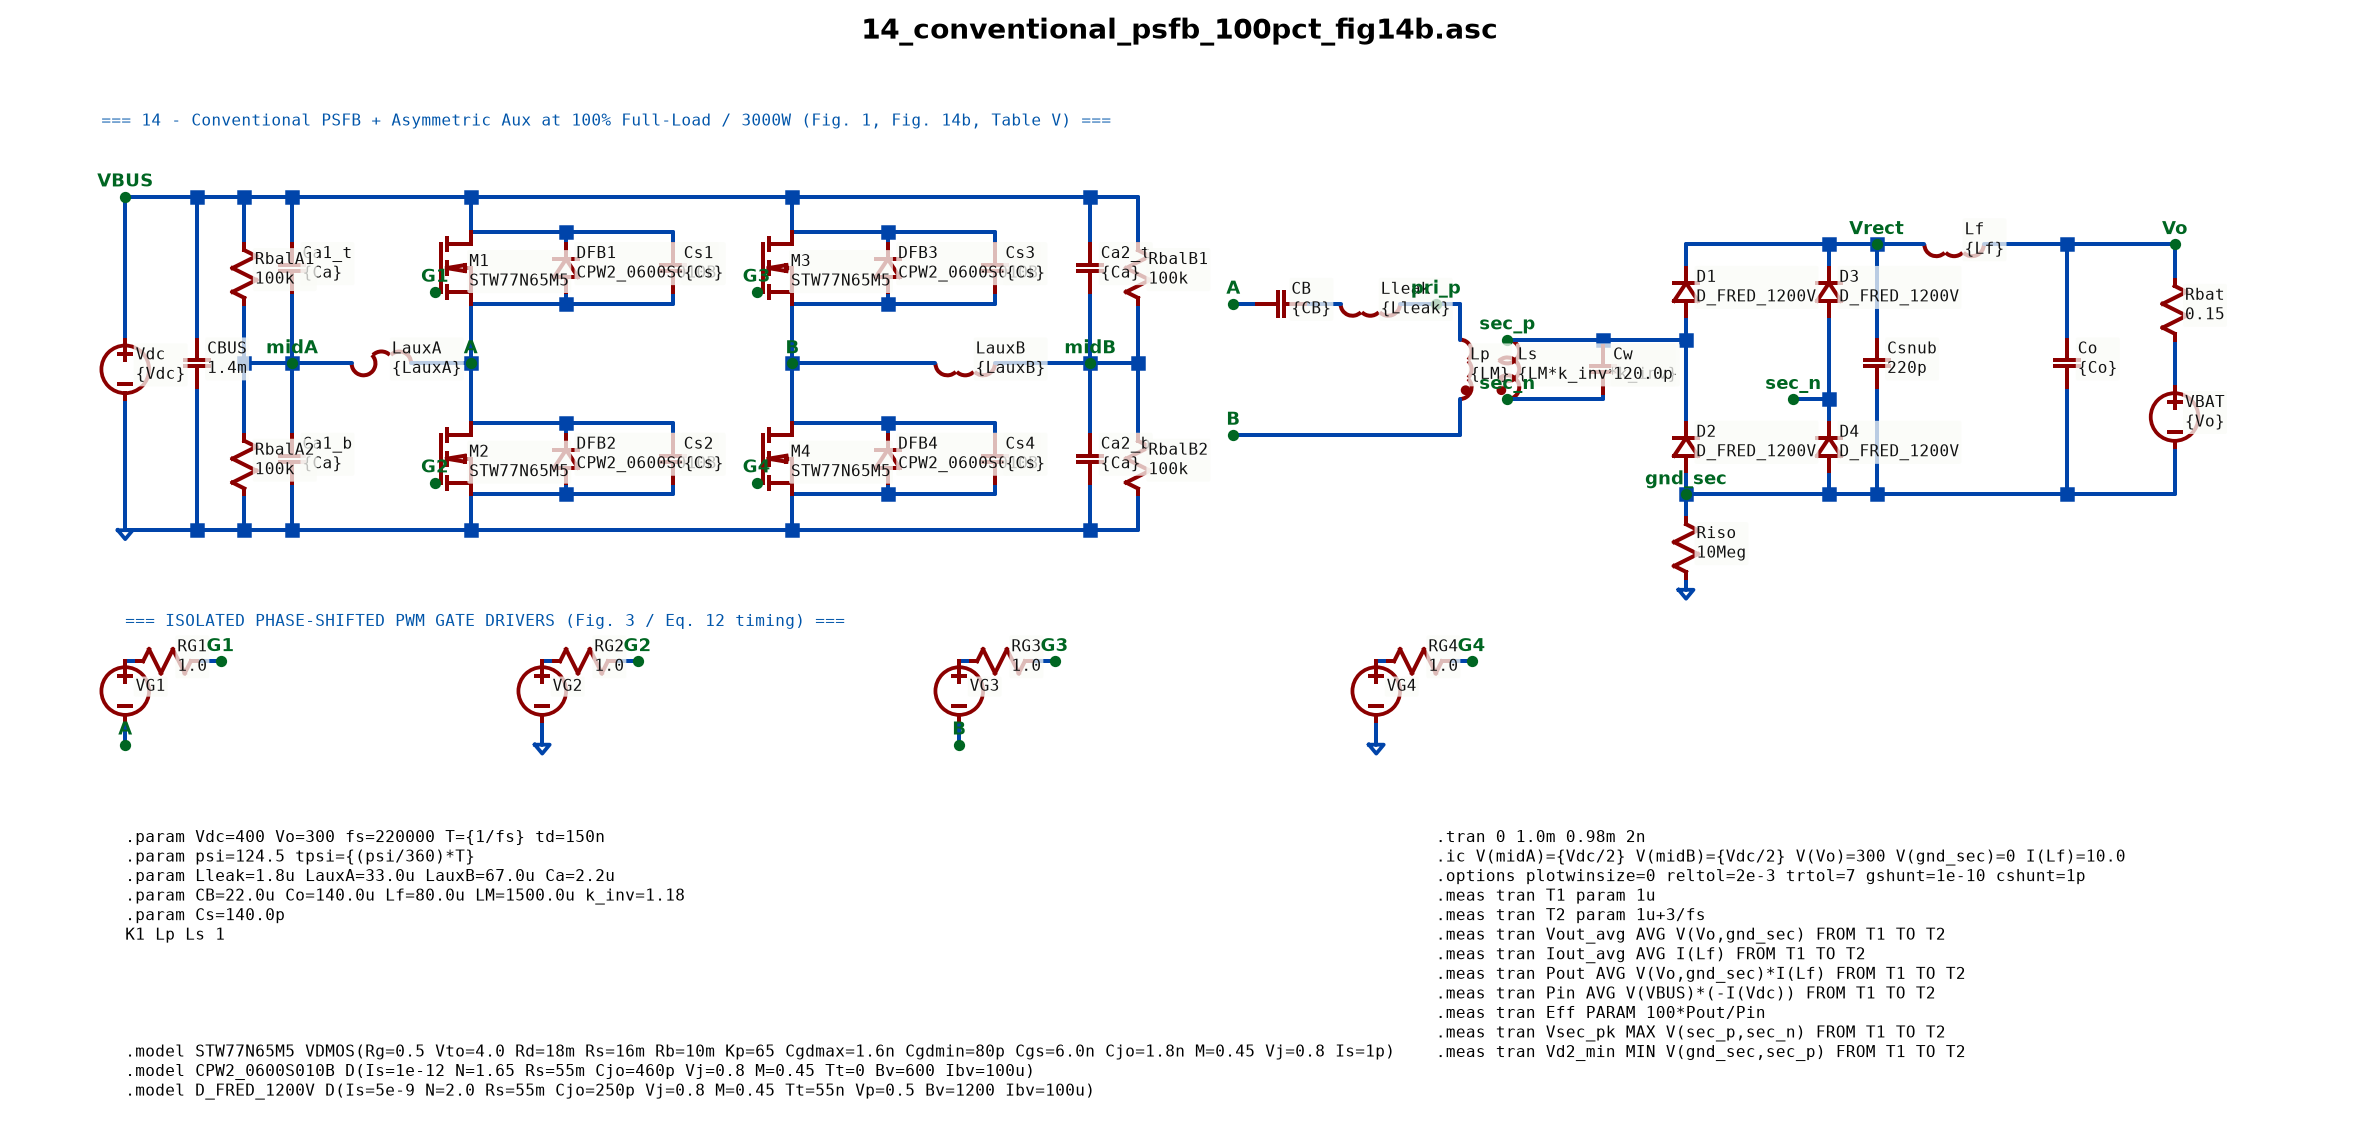
\includegraphics[width=\textwidth,height=3.65cm,keepaspectratio]{14_conventional_psfb_100pct_fig14b.png}\\[-1mm]
      {\tiny\color{MutedGray}Schema LTspice PSFB convenzionale + ausiliario asimmetrico (Tabella V)}

      \vspace*{2.5mm}
      \begin{tikzpicture}[scale=0.75, transform shape,
        bx/.style={draw=AlertRed, fill=AlertBg, rounded corners=2pt, minimum height=0.68cm, align=center, font=\scriptsize\bfseries},
        ar/.style={-{Stealth[length=2mm]}, thick, AlertRed}
      ]
        \node[bx] (l1) {Induttore $L_{leak}$\\[-1pt]\tiny Generatore corrente 1};
        \node[bx, right=4.5mm of l1, fill=white] (db) {Ponte Diodi\\[-1pt]\tiny $D_1\text{--}D_4$ ($Q_{rr}$)};
        \node[bx, right=4.5mm of db] (l2) {Induttore $L_f$\\[-1pt]\tiny Generatore corrente 2};
        \node[bx, right=4.0mm of l2, draw=MutedGray, fill=LightBg] (co) {$C_o$ ($140\uF$)\\[-1pt]\tiny dopo $L_f$};
        \draw[ar] (l1) -- (db);
        \draw[ar] (db) -- (l2);
        \draw[ar, MutedGray] (l2) -- (co);
        \node[above=0.5mm of db, font=\scriptsize\bfseries, color=AlertRed] {SCONTRO $\Rightarrow L\frac{di}{dt} > 950\V$!};
      \end{tikzpicture}
    \end{column}
    \begin{column}{0.44\textwidth}
      \scriptsize
      \textbf{\color{PrimaryBlue}I 3 difetti strutturali del PSFB (\emph{voltage-driven}):}
      \begin{enumerate}\setlength{\itemsep}{3.5pt}
        \item \textbf{\color{AlertRed}Sovratensioni distruttive sui diodi:}\\
              $L_{leak}$ ($1.8\uH$) e $L_f$ ($80\uH$) sono \textbf{due generatori di corrente in serie} attraverso il ponte a diodi. Ogni commutazione (aggravata da $Q_{rr}$ e $C_w, C_j$) crea picchi di \textbf{636--961\,V} (per $V_o=300\V$!), imponendo diodi Si da \textbf{1200\,V} (alta $V_F$, alta $Q_{rr}$) e snubber R-C-D dissipativi.
        \item \textbf{\color{AlertRed}Perdita ZVS a vuoto e ausiliario asimmetrico:}\\
              $\frac{1}{2}L_{leak}I_p^2$ non basta a scaricare $C_{oss}$ a basso carico $\Rightarrow$ \emph{hard switching} e rischio \emph{shoot-through}. Con un ausiliario (Tab.\,V), sulla \emph{leading leg} serve $L_{AUX,A}=33\uH$ (met\`a di $L_{AUX,B}=67\uH$) per vincere la corrente di dispersione negativa: corrente doppia e \textbf{perdite $4\times$}!
        \item \textbf{\color{AlertRed}Freewheeling e perdita di duty-cycle:}\\
              Con $v_{AB}=0$, la corrente riflessa ricircola nel primario e nei diodi (perdite di conduzione) e ritarda la salita di $v_{sec}$ (\emph{duty-cycle loss}).
      \end{enumerate}
    \end{column}
  \end{columns}
\end{frame}

% --- SLIDE 5 ---
\begin{frame}{Evidenza LTspice del PSFB Convenzionale: Picchi e Freewheeling (Fig.\,14)}{Replica LTspice di Fig.\,14(a) al 10\% e Fig.\,14(b) al 100\% di carico (Tabella V)}
  \begin{columns}[T,onlytextwidth]
    \begin{column}{0.58\textwidth}
      \centering
      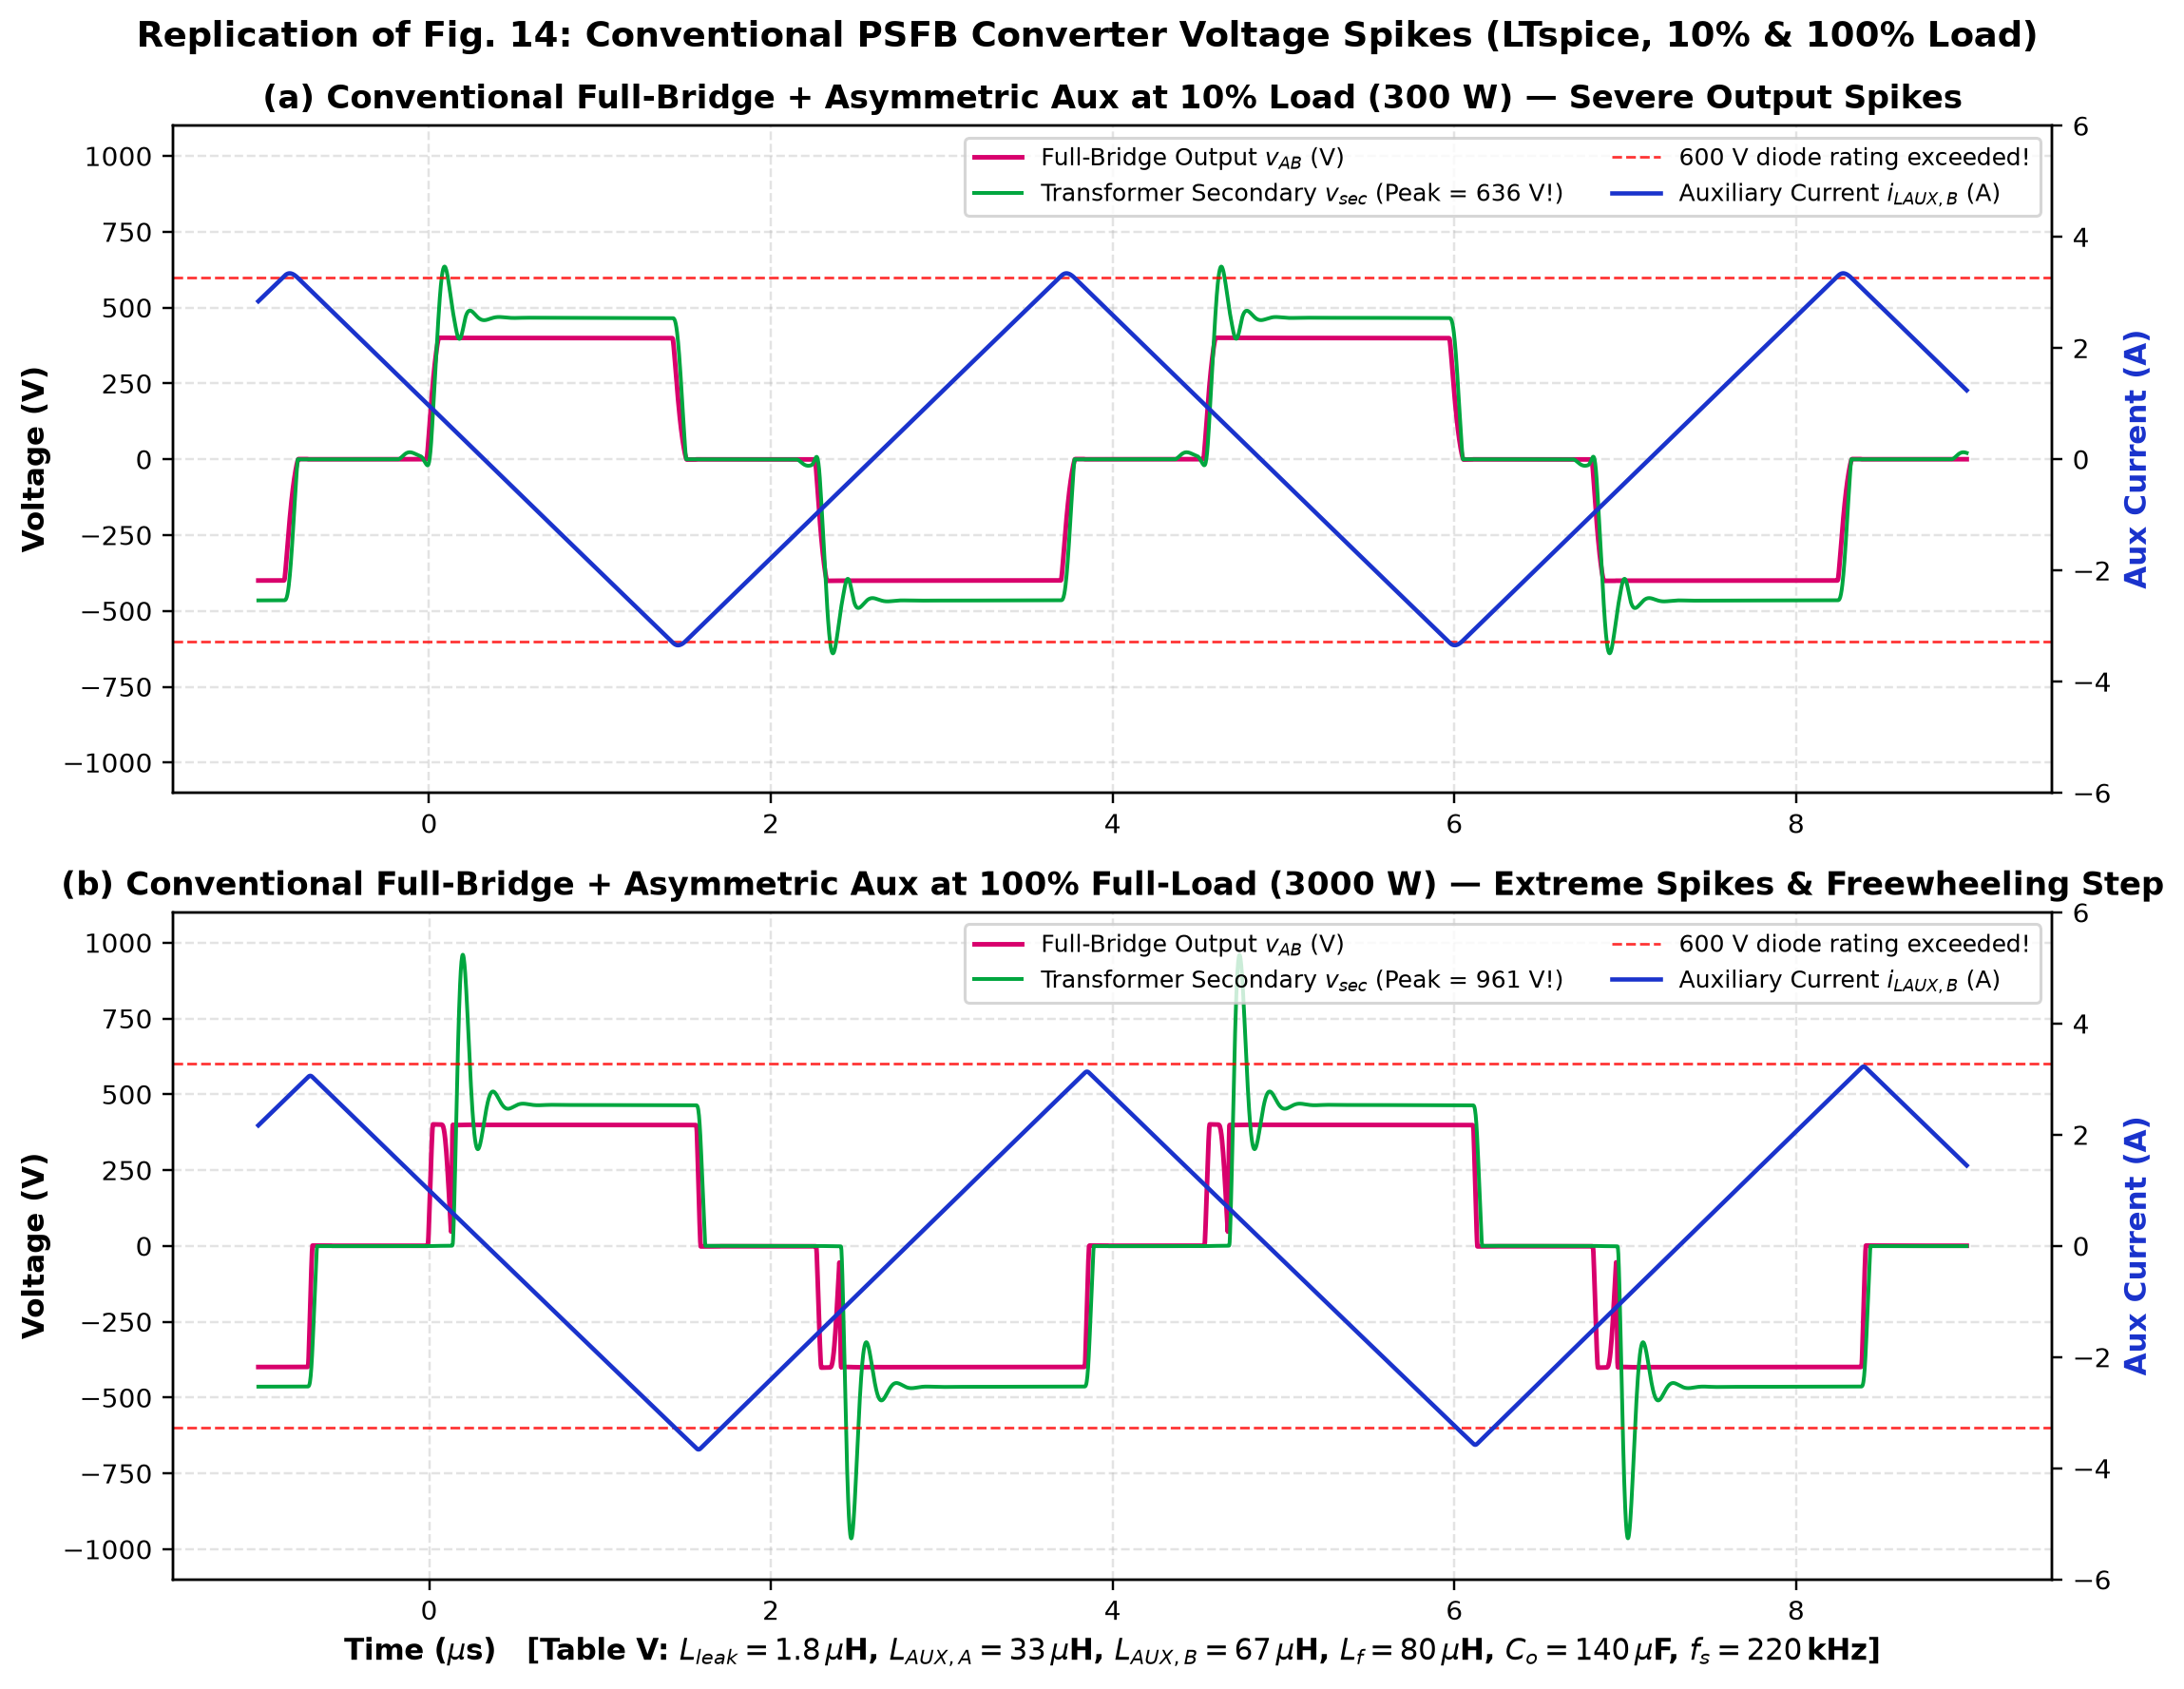
\includegraphics[width=\textwidth,height=6.05cm,keepaspectratio]{fig14_conventional_fb_10_100pct.png}
    \end{column}
    \begin{column}{0.40\textwidth}
      \scriptsize
      \textbf{\color{PrimaryBlue}Lettura del grafico (\texttt{fig14\_conventional\_fb}):}
      \begin{itemize}\setlength{\itemsep}{2.5pt}
        \item \textbf{Tracce}: $v_{AB}$ (magenta, $\pm 400\V$), tensione secondaria $v_{sec}$ (verde, sui diodi), corrente ausiliaria $i_{LAUX,B}$ (blu, triangolare), soglia rossa a $\pm 600\V$.
        \item \textbf{Pannello (a) --- 10\% carico ($335\W$, $\psi=114^\circ$)}: gi\`a a basso carico $v_{sec}$ presenta un picco oscillatorio a \textbf{636\,V} ($V_{D2,\min}=-634.7\V$), sfondando il limite dei diodi da $600\V$. Efficienza: $\eta=92.24\%$.
        \item \textbf{Pannello (b) --- 100\% carico ($2904\W$, $\psi=124.5^\circ$)}: il picco esplode a \textbf{961\,V} ($V_{D2,\min}=-959.2\V$, oltre $3\times V_o$!) con forte ringing ad alta frequenza (sorgente primaria di \textbf{EMI}).
        \item \textbf{Gradino di \emph{duty-cycle loss}}: visibile in (b) sul fronte di salita --- $v_{AB}$ \`e gi\`a a $+400\V$ ma $v_{sec}$ resta a $0\V$ finch\'e $i_{Lleak}$ non raggiunge la corrente riflessa di $L_f$!
      \end{itemize}
      \vspace*{1mm}
      \begin{warnbox}
        \textbf{Conclusione:} anche con snubber R-C ($150\Ohm/220\pF$) e diodi da 1200\,V, il PSFB convenzionale resta rumoroso e inefficiente ($\eta=94.33\%$ al 100\%).
      \end{warnbox}
    \end{column}
  \end{columns}
\end{frame}

% ==============================================================================
% SEZIONE 2: TOPOLOGIA PROPOSTA E RUOLO DI OGNI COMPONENTE
% ==============================================================================
\section{2. Topologia e Componenti}

% --- SLIDE 6 ---
\begin{frame}{Architettura della Topologia Proposta (Fig.\,2) e Schema Master LTspice}{Le due innovazioni chiave che risolvono tutti i limiti del PSFB}
  \centering
  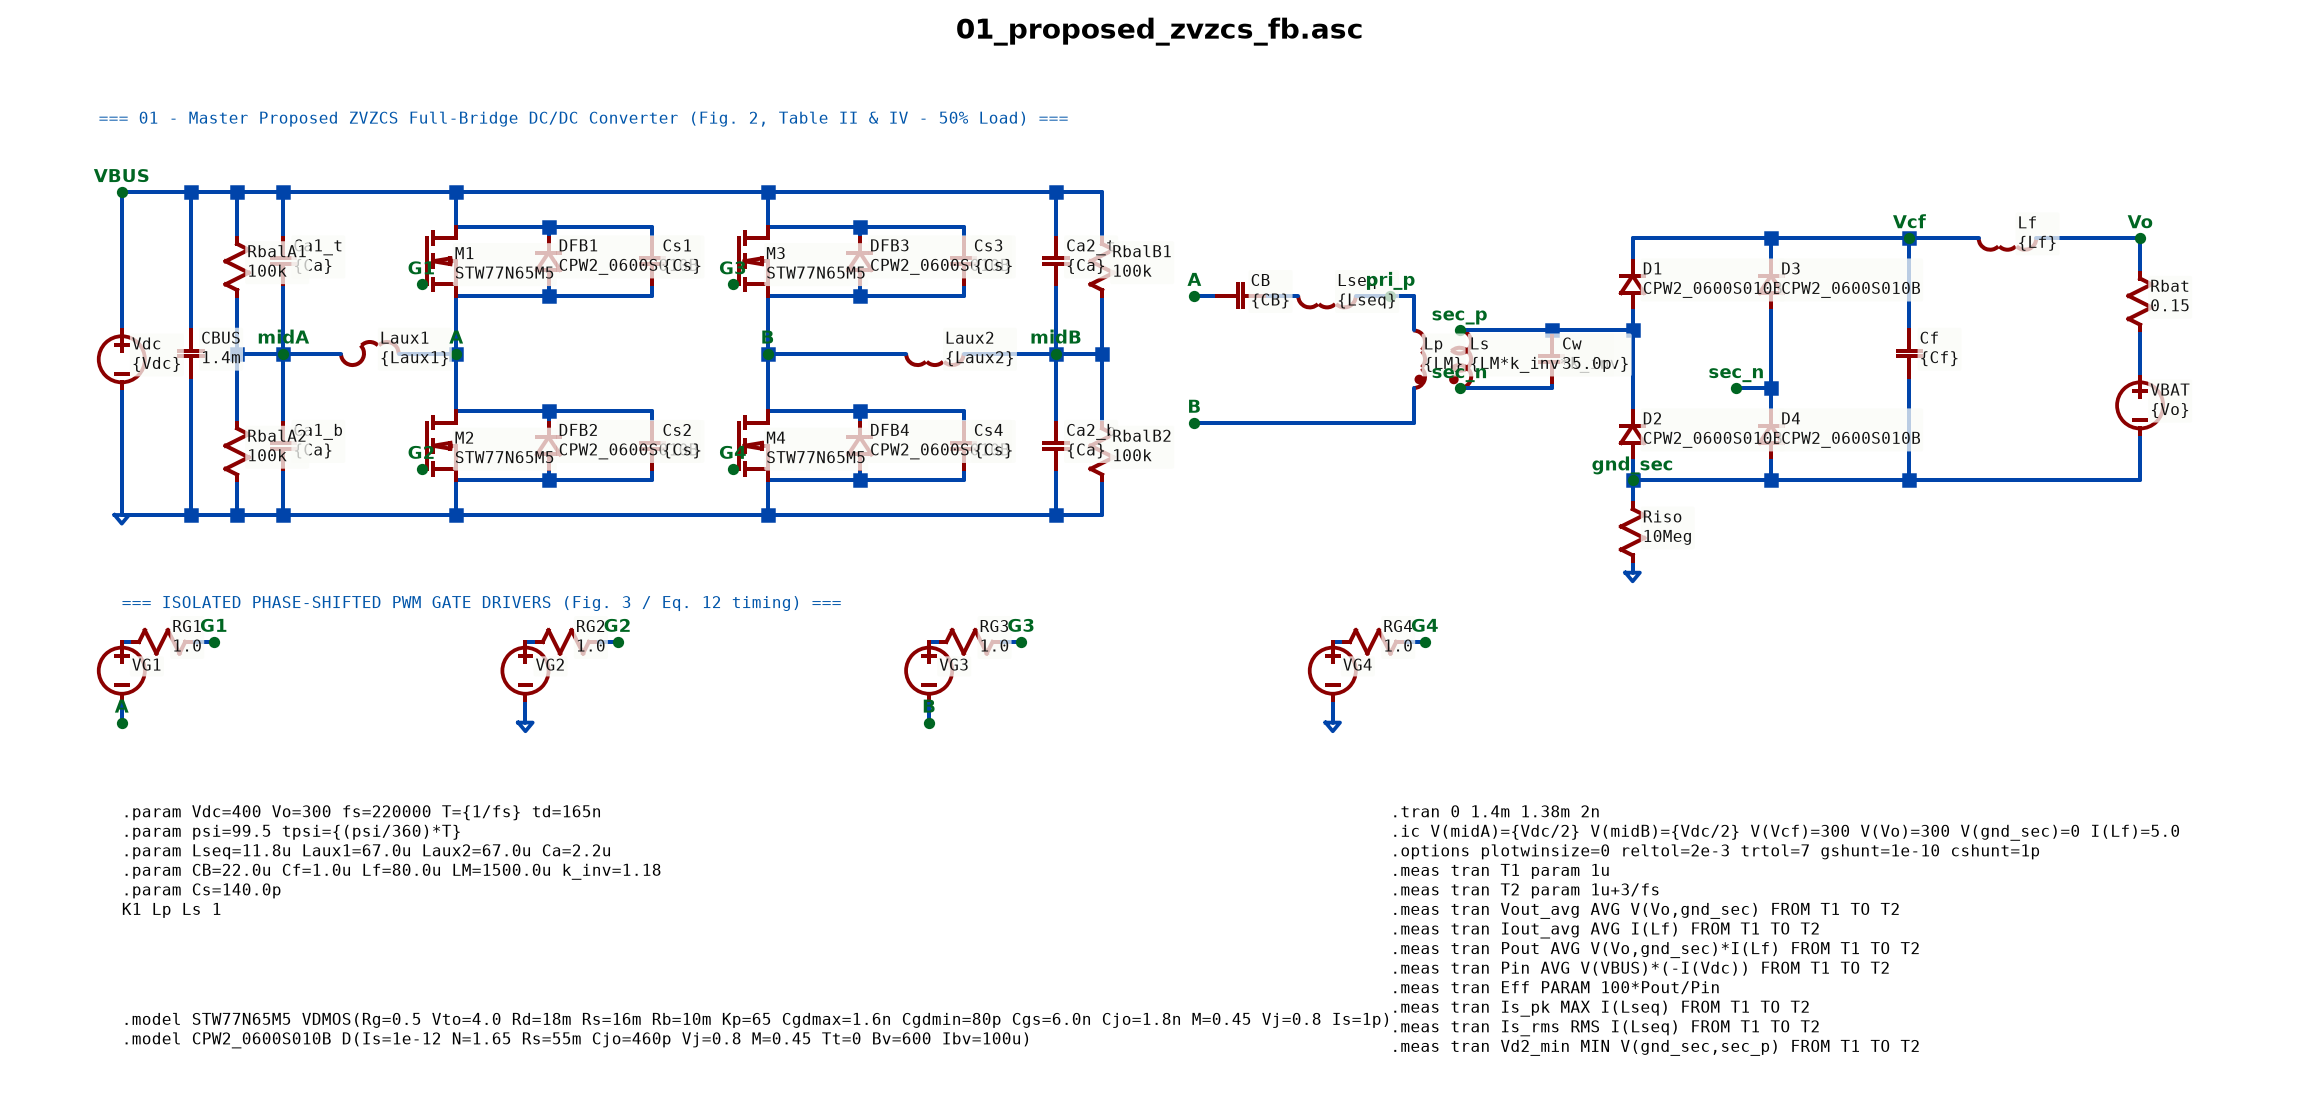
\includegraphics[width=0.80\textwidth,height=4.05cm,keepaspectratio]{01_proposed_zvzcs_fb.png}\\[-1mm]
  {\tiny\color{MutedGray}Schema master LTspice (\texttt{01\_proposed\_zvzcs\_fb.asc}): ponte intero, ausiliario simmetrico, $C_B$, $L_{seq}$, trasformatore $1:1.18$, ponte SiC, $C_f$ prima di $L_f$.}

  \vspace*{1.5mm}
  \begin{columns}[T,onlytextwidth]
    \begin{column}{0.49\textwidth}
      \begin{okbox}[title={Innovazione 1: Raddrizzatore Current-Driven ($L_{seq}$ + $C_f$ prima di $L_f$)}]
        \begin{itemize}\setlength{\itemsep}{1.5pt}
          \item $L_{seq}=11.8\uH$ (integrato nella dispersione) lavora in \textbf{DCM} e agisce da sorgente di corrente impulsiva.
          \item $C_f=1\uF$ posto subito dopo $D_1\text{--}D_4$ (e \textbf{prima} di $L_f$) fissa rigidamente la tensione di blocco a \textbf{$V_o=300\V$} $\Rightarrow$ zero spike, diodi SiC \textbf{600\,V}, \textbf{ZCS naturale} e \textbf{zero freewheeling}!
        \end{itemize}
      \end{okbox}
    \end{column}
    \begin{column}{0.49\textwidth}
      \begin{formulabox}[title={Innovazione 2: Circuito Ausiliario Passivo Simmetrico}]
        \begin{itemize}\setlength{\itemsep}{1.5pt}
          \item In DCM, quando commuta la gamba \emph{leading} ($M_1, M_2$), $i_s$ parte da \textbf{zero}: non c'\`e alcuna corrente negativa da compensare!
          \item Entrambi i rami usano $L_{AUX1}=L_{AUX2}=67\uH$ identici ($I_{PA}=I_{PB}=3.39\A$, $1.96\A_{\text{rms}}$): garantiscono \textbf{ZVS dal 100\% allo 0\%} e \textbf{ZVZCS} sulla \emph{leading leg}!
        \end{itemize}
      \end{formulabox}
    \end{column}
  \end{columns}
\end{frame}

% --- SLIDE 7 ---
\begin{frame}{Ruolo Fisico di Ogni Singolo Componente (1/2): Primario e Ausiliario}{Analisi dettagliata di sorgente, ponte intero, semiconduttori, driver e rami ZVS}
  \scriptsize
  \setlength{\tabcolsep}{3.5pt}
  \renewcommand{\arraystretch}{1.20}
  \begin{tabular}{@{}>{\raggedright\arraybackslash}p{2.25cm}>{\raggedright\arraybackslash}p{2.85cm}>{\raggedright\arraybackslash}p{8.8cm}@{}}
    \toprule
    \textbf{Componente} & \textbf{Modello / Valore} & \textbf{Ruolo fisico esatto nel convertitore} \\
    \midrule
    Bus DC $V_{dc}$, $C_{BUS}$ & $400\V_{\text{DC}}$, $1.4\mF$ & Alimentazione DC dallo stadio PFC; $C_{BUS}$ abbatte il ripple a $2f_{\text{rete}}$ ($100/120\,\text{Hz}$) e fornisce percorso a bassa impedenza alle correnti impulsive a $220\kHz$. \\
    MOSFET $S_1, S_2$ (\emph{Leading}) e $S_3, S_4$ (\emph{Lagging}) & \texttt{STW77N65M5} (650\,V, 65\,A, $R_{ds,\text{on}}=33\mOhm$) & Convertono $V_{dc}$ in onda quasi-quadra $v_{AB}$ a $220\kHz$. Lo sfasamento $\psi$ tra gamba \emph{leading} e \emph{lagging} controlla la potenza erogata alla batteria. \\
    Diodi antiparallelo $D_{FB1}\text{--}D_{FB4}$ & \texttt{CPW2-0600S010B} SiC (600\,V, 10\,A) \textbf{bare-die} & Bypassano il lento \emph{body-diode} dei MOSFET super-junction durante $t_d$ (conducono la corrente reattiva ZVS). Il montaggio \emph{bare-die} azzera l'induttanza parassita dei pin. \\
    Capacit\`a di commutazione $C_{s1}\text{--}C_{s4}$ & $C_s=140\pF$ ($C_{so,\text{eff}}\approx 650\pF$ tot.) & Sommate a $C_{oss}$ e $C_{j,DFB}$, rallentano $dv/dt$ al turn-off riducendo le perdite di spegnimento; vengono scaricate a $0\V$ durante $t_d$ per garantire lo ZVS. \\
    Gate Driver $DR$ & \texttt{UCC27322D} (9\,A picco, $R_g=1\Ohm$) & Elevata corrente di picco per caricare/scaricare rapidamente la gate ($C_{gs}, C_{gd}$), accorciando i fronti e minimizzando le perdite di turn-off a $220\kHz$. \\
    Partitori $C_{a1}, C_{a2}$ (+ $R_{bal}$) & $2.2\uF$ (300\,V) + $100\kOhm$ & Fissano due nodi di tensione rigidi a $V_{dc}/2 = 200\V$ (\texttt{midA}, \texttt{midB}) rispetto a cui lavorano gli induttori ausiliari ($R_{bal}$ assicura bilanciamento DC). \\
    Induttori ausiliari $L_{AUX1}, L_{AUX2}$ & $67\uH$, $67\uH$ ($2\A_{\text{rms}}$, \textbf{simmetrici}) & Sottoposti a $\pm V_{dc}/2=\pm 200\V$, generano una corrente triangolare reattiva $\pm 3.39\A$ \textbf{indipendente dal carico} che scarica $2C_{so}$ in $t_d$ $\Rightarrow$ ZVS anche a 0\%! \\
    \bottomrule
  \end{tabular}
\end{frame}

% --- SLIDE 8 ---
\begin{frame}{Ruolo Fisico di Ogni Singolo Componente (2/2): Magnetica, Raddrizzatore e Uscita}{Analisi dettagliata di $C_B$, $L_{seq}$, trasformatore, ponte SiC, $C_f$, $L_f$ e batteria}
  \scriptsize
  \setlength{\tabcolsep}{3.5pt}
  \renewcommand{\arraystretch}{1.18}
  \begin{tabular}{@{}>{\raggedright\arraybackslash}p{2.25cm}>{\raggedright\arraybackslash}p{2.85cm}>{\raggedright\arraybackslash}p{8.8cm}@{}}
    \toprule
    \textbf{Componente} & \textbf{Modello / Valore} & \textbf{Ruolo fisico esatto nel convertitore} \\
    \midrule
    Condensatore DC-blocking $C_B$ & $22\uF$ (omesso in Tab.\,II) & Blocca ogni offset DC di $v_{AB}$ (dovuto ad asimmetrie di driver/duty), impedendo la \textbf{saturazione magnetica} del trasformatore. $f_{r,CB}\approx 9.9\kHz \ll 220\kHz$ (cortocircuito AC). \\
    Induttore serie $L_{seq} = L_s + L_{leak}$ & $11.8\uH$ ($12.6\A_{\text{rms}}$), integrato nel trasf. & Determina la pendenza $di_s/dt$ e l'energia trasferita per ciclo. Operando in DCM trasforma il primario in sorgente di corrente ed elimina il conflitto induttivo con l'uscita. \\
    Trasformatore d'isolamento & $k = N_p/N_s = 1/1.18$, $L_M=1.5\mH$, $C_w=35\pF$ & Assicura \textbf{isolamento galvanico} rete--batteria. Rapporto \textbf{elevatore} ($1:1.18$) per coprire $V_{BAT}=431\V$ da $400\V$. $L_M$ alta minimizza la corrente magnetizzante; $C_w$ \`e la capacit\`a parassita secondaria. \\
    Ponte diodi d'uscita $D_1\text{--}D_4$ & \texttt{CPW2-0600S010B} SiC (600\,V, 10\,A, $Q_{rr}=0$) & Raddrizzano la corrente impulsiva secondaria $i_{DB}$ ($V_d\approx 1.5\V$). Spegnimento in \textbf{ZCS naturale} quando $i_s\to 0$: zero perdite di recupero inverso! (In Tab.\,IV chiamati per refuso \texttt{D\_PFC}). \\
    Condensatore di clamping $C_f$ & $1\uF$ ($400\V_{\text{DC}}$), \textbf{prima} di $L_f$ & Cuore del raddrizzatore \emph{current-driven}: fissa $v_{D,\text{rev}} \le V_o$ (clamping rigido, zero spike, niente snubber!) e sostiene $L_f$ durante il Modo VII (intervallo DCM). \\
    Induttore di filtro d'uscita $L_f$ & $80\uH$ ($10\A_{\text{DC}}$), \textbf{dopo} $C_f$ & Filtra il piccolo ripple su $C_f$ ($\Delta V_{Cf}\approx 5.7\V$) consegnando una corrente continua e pulita $I_o$ alla batteria HV senza impulsi di carica. \\
    Batteria HV (o $R_e$) & $V_{BAT}=235\text{--}431\V$ ($R_{bat}=0.15\Ohm$) & Carico reale EV (test a $300\V$, $I_o=0\text{--}10\A$). Nello sweep di guadagno (Fig.\,7) sostituita da carico resistivo $R_e \in [30, 300]\Ohm$ + $C_{out}=47\uF$. \\
    \bottomrule
  \end{tabular}
\end{frame}

% --- SLIDE 9 ---
\begin{frame}{Confronto Completo dei Parametri: Topologia Proposta vs.\ Convenzionale}{Sintesi di Tabelle I, II, IV, V del paper e dei parametri parassiti/omessi validati in LTspice}
  \centering
  \scriptsize
  \setlength{\tabcolsep}{3.5pt}
  \renewcommand{\arraystretch}{1.16}
  \begin{tabular}{@{}lcccc@{}}
    \toprule
    \textbf{Parametro} & \textbf{Simbolo} & \textbf{Topologia Proposta} & \textbf{PSFB Convenzionale} & \textbf{Impatto Fisico / Note} \\
    \midrule
    Potenza / Bus DC & $P_o$ / $V_{dc}$ & $3\kW$ / $400\V$ & $3\kW$ / $400\V$ & Identici \\
    Tensione uscita (test) & $V_o$ & $235\text{--}431\V$ ($300\V$) & $300\V$ & In Figg.\,16--20 reale $\approx 355\V$! \\
    Frequenza switching & $f_s$ ($T_s$) & $220\kHz$ ($4.545\us$) & $220\kHz$ ($4.545\us$) & In Fig.\,14 reale $\approx 150\kHz$! \\
    Rapporto spire ($N_p:N_s$) & $k$ & $1:1.18$ ($0.8475$) & $1:1.18$ ($0.8475$) & Elevatore per coprire $431\V$ \\
    Induttanza serie/disp. & $L_{seq}$ / $L_{leak}$ & \textbf{$11.8\uH$} ($12.6\A_{\text{rms}}$) & $1.8\uH$ & Integrata nel trasformatore \\
    Induttori ausiliari & $L_{AUX1,2}$ & \textbf{$67\uH,\;67\uH$} (simm.) & \color{AlertRed}$33\uH,\;67\uH$ (asimm.) & Perdite $4\times$ su ramo leading conv. \\
    Capacit\`a partitori aux & $C_{a1,2}$ & $2.2\uF$ ($300\V$) & $2.2\uF$ & Punto medio a $V_{dc}/2=200\V$ \\
    Condensatore uscita & $C_f$ / $C_o$ & \textbf{$1\uF$ prima di $L_f$} & $140\uF$ dopo $L_f$ & Clamping rigido vs spike $>950\V$ \\
    Induttore filtro uscita & $L_f$ & $80\uH$ ($10\A_{\text{DC}}$) & $80\uH$ & Corrente DC pulita in batteria \\
    MOSFET ponte intero & $S_1\text{--}S_4$ & \texttt{STW77N65M5} & \texttt{STW77N65M5} & + $D_{FB}$ SiC bare-die + driver 9\,A \\
    Diodi raddrizzatore & $D_1\text{--}D_4$ & \textbf{SiC 600\,V} ($Q_{rr}=0$) & \color{AlertRed}Si 1200\,V ($T_t=55\ns$) & Stress $-68\%$, zero snubber \\
    Snubber R-C uscita & $R_s, C_s$ & \textbf{Assente (0\,W)} & $120\text{--}150\Ohm$, $220\text{--}330\pF$ & Forte fonte di perdite nel conv. \\
    Omessi Tab.\,II (SPICE) & $C_B, L_M, t_d, C_w$ & $22\uF, 1.5\mH, 165\ns, 35\pF$ & $22\uF, 1.5\mH, 150\ns, 120\pF$ & Fisicamente necessari in LTspice \\
    \bottomrule
  \end{tabular}
\end{frame}

% ==============================================================================
% SEZIONE 3: PERIODO, TON/TOFF, 7 MODI E RISONANZE
% ==============================================================================
\section{3. Periodo, 7 Modi e Risonanze}

% --- SLIDE 10 ---
\begin{frame}{Periodo $T_s$, Modulazione Phase-Shift, $t_{on}$, $t_{off}$ e Regimi DCM/BCM/CCM}{Come varia la corrente $i_s(t)$ nel semiperiodo $T_s/2 = 2.273\us$ al crescere di $\psi$}
  \begin{columns}[T,onlytextwidth]
    \begin{column}{0.53\textwidth}
      \centering
      \begin{tikzpicture}[scale=0.72, transform shape]
        % --- Assi v_AB ---
        \draw[->, gray] (0,3.2) -- (8.8,3.2) node[right, font=\scriptsize] {$t$};
        \node[left, font=\scriptsize\bfseries, color=PrimaryBlue] at (0,3.85) {$v_{AB}$};
        \draw[very thick, AccentBlue] (0,3.2) -- (0.3,3.2) -- (0.55,4.2) -- (3.2,4.2) -- (3.35,3.2) -- (5.5,3.2) -- (5.75,2.2) -- (8.4,2.2);
        \node[left, font=\tiny] at (0,4.2) {$+V_{dc}$};
        \node[left, font=\tiny] at (0,2.2) {$-V_{dc}$};
        % Quote t_d e t_on
        \draw[<->, thin, AlertRed] (0.3,4.45) -- node[above, font=\tiny\bfseries] {$t_d$} (0.55,4.45);
        \draw[<->, thin, PrimaryBlue] (0.55,4.45) -- node[above, font=\tiny\bfseries] {$t_{on}=\frac{\psi}{\omega_s}-t_d$} (3.2,4.45);
        \draw[dashed, gray] (0.3,0.0) -- (0.3,4.5);
        \draw[dashed, gray] (0.55,0.0) -- (0.55,4.5);
        \draw[dashed, gray] (3.2,0.0) -- (3.2,4.5);
        \draw[dashed, gray] (4.5,0.0) -- (4.5,4.5);
        \draw[dashed, gray] (5.5,0.0) -- (5.5,4.5);

        % --- Assi i_s ---
        \draw[->, gray] (0,0.8) -- (8.8,0.8) node[right, font=\scriptsize] {$t$};
        \node[left, font=\scriptsize\bfseries, color=GoodGreen] at (0,1.4) {$i_s$};
        % Curva DCM
        \draw[very thick, GoodGreen] (0,0.8) -- (0.55,0.8) -- (3.2,2.05) -- (4.5,0.8) -- (5.5,0.8) -- (5.75,0.8) -- (8.4,-0.35);
        % Curva BCM tratteggiata
        \draw[thick, dashed, WarnAmber] (0.55,0.8) -- (3.85,2.35) -- (5.5,0.8);
        % Curva CCM punteggiata
        \draw[thick, dotted, AlertRed] (0.3,0.15) -- (0.65,0.8) -- (4.2,2.45) -- (5.5,1.45) -- (5.8,0.8);

        % Quote t_off e Modo VII
        \draw[<->, thin, GoodGreen] (3.2,0.35) -- node[below, font=\tiny\bfseries] {$t_{off}$} (4.5,0.35);
        \draw[<->, thin, MutedGray] (4.5,0.35) -- node[below, font=\tiny] {M\,VII} (5.5,0.35);
        \draw[<->, thin, PrimaryBlue] (0.3,-0.15) -- node[below, font=\tiny\bfseries] {Semiperiodo $T_s/2 = 2.273\us$} (5.5,-0.15);

        % Etichette t0..t7
        \node[font=\tiny] at (0.28,0.62) {$t_0$};
        \node[font=\tiny] at (0.63,0.62) {$t_2$};
        \node[font=\tiny] at (3.2,0.62) {$t_3$};
        \node[font=\tiny] at (4.5,0.62) {$t_6$};
        \node[font=\tiny] at (5.5,0.62) {$t_7$};
        \node[font=\tiny\bfseries, color=GoodGreen] at (1.50,1.88) {$+12.1\,\text{A}/\mu\text{s}$};
        \node[font=\tiny\bfseries, color=GoodGreen] at (4.85,1.42) {$-21.8\,\text{A}/\mu\text{s}$};

        % Legenda in alto a destra
        \draw[very thick, GoodGreen] (5.7,4.28) -- (6.2,4.28) node[right, font=\tiny, color=TextDark] {DCM ($t_{on}+t_{off}<T_s/2$)};
        \draw[thick, dashed, WarnAmber] (5.7,3.92) -- (6.2,3.92) node[right, font=\tiny, color=TextDark] {BCM ($t_{on}+t_{off}=T_s/2$)};
        \draw[thick, dotted, AlertRed] (5.7,3.56) -- (6.2,3.56) node[right, font=\tiny, color=TextDark] {CCM ($i_s\neq 0$ a $t_7$, no ZCS)};
      \end{tikzpicture}

      \vspace*{1.5mm}
      \begin{formulabox}[title={Bilancio Volt-Secondi su $L_{seq}$ e rapporto $t_{off}/t_{on}$}]
        Durante $t_{on}$: $v_{Lseq} = V_{dc} - k(V_o+2V_d) = +143.2\V$; durante $t_{off}$: $-256.8\V$.
        \begin{gather*}
          \bigl[V_{dc}-k(V_o+2V_d)\bigr]\,t_{on} = k(V_o+2V_d)\,t_{off} \\
          \frac{t_{off}}{t_{on}} = \frac{V_{dc}-k(V_o+2V_d)}{k(V_o+2V_d)} = \frac{143.2}{256.8} = \mathbf{0.558}
        \end{gather*}
      \end{formulabox}
    \end{column}
    \begin{column}{0.45\textwidth}
      \scriptsize
      \textbf{\color{PrimaryBlue}Controllo Phase-Shift PWM ($f_s = 220\kHz$):}
      \begin{itemize}\setlength{\itemsep}{2pt}
        \item Periodo completo $T_s = 1/f_s = \mathbf{4.545\us}$ ($\omega_s = 2\pi f_s$); ogni semiperiodo vale $T_s/2 = \mathbf{2.273\us}$ ($180^\circ$).
        \item Ogni gamba commuta al $50\%$ meno il \textbf{dead-time $t_d = 165\ns$} ($\approx 13^\circ$), per prevenire lo \emph{shoot-through} e consentire lo ZVS.
        \item Lo sfasamento $\psi \in [0^\circ, 180^\circ]$ tra gamba \emph{leading} ($S_1, S_2$) e \emph{lagging} ($S_3, S_4$) fissa la durata attiva:
          \[
            t_{on} = \frac{\psi}{\omega_s} - t_d = \frac{\psi}{360^\circ}\,T_s - t_d
          \]
        \item Durata totale dell'impulso triangolare in DCM:
          \[
            t_{on} + t_{off} = t_{on}\,\frac{V_{dc}}{k(V_o+2V_d)} \approx 1.558\,t_{on}
          \]
      \end{itemize}
      \vspace*{1mm}
      \begin{okbox}[title={I 3 Regimi di Conduzione}]
        \begin{itemize}\setlength{\itemsep}{1.2pt}
          \item \textbf{DCM} ($t_{on}+t_{off} < T_s/2$): $i_s$ torna a $0\A$ prima di $t_7$; Modo VII presente, \textbf{ZCS} diodi e \textbf{ZVZCS} \emph{leading}.
          \item \textbf{BCM} ($t_{on}+t_{off} = T_s/2$): soglia critica $t_{on,\text{BCM}}=\frac{kV_o}{V_{dc}}\frac{T_s}{2}\approx 1.445\us$ ($\psi\approx 120^\circ$).
          \item \textbf{CCM} ($t_{on}+t_{off} > T_s/2$): $i_s$ inverte bruscamente con pendenza $(V_{dc}+kV_o)/L_{seq}\approx 55.7\A/\us$ $\Rightarrow$ \textbf{ZCS perso}!
        \end{itemize}
      \end{okbox}
    \end{column}
  \end{columns}
\end{frame}

% --- SLIDE 11 ---
\begin{frame}{Panoramica dei 7 Modi di Funzionamento: Tutte le 12 Tracce (Fig.\,3)}{Replica LTspice ad alta risoluzione ($1\ns$) di Fig.\,3 al 50\% di carico DCM ($\psi=99.5^\circ$, $t_d=165\ns$)}
  \begin{columns}[T,onlytextwidth]
    \begin{column}{0.38\textwidth}
      \centering
      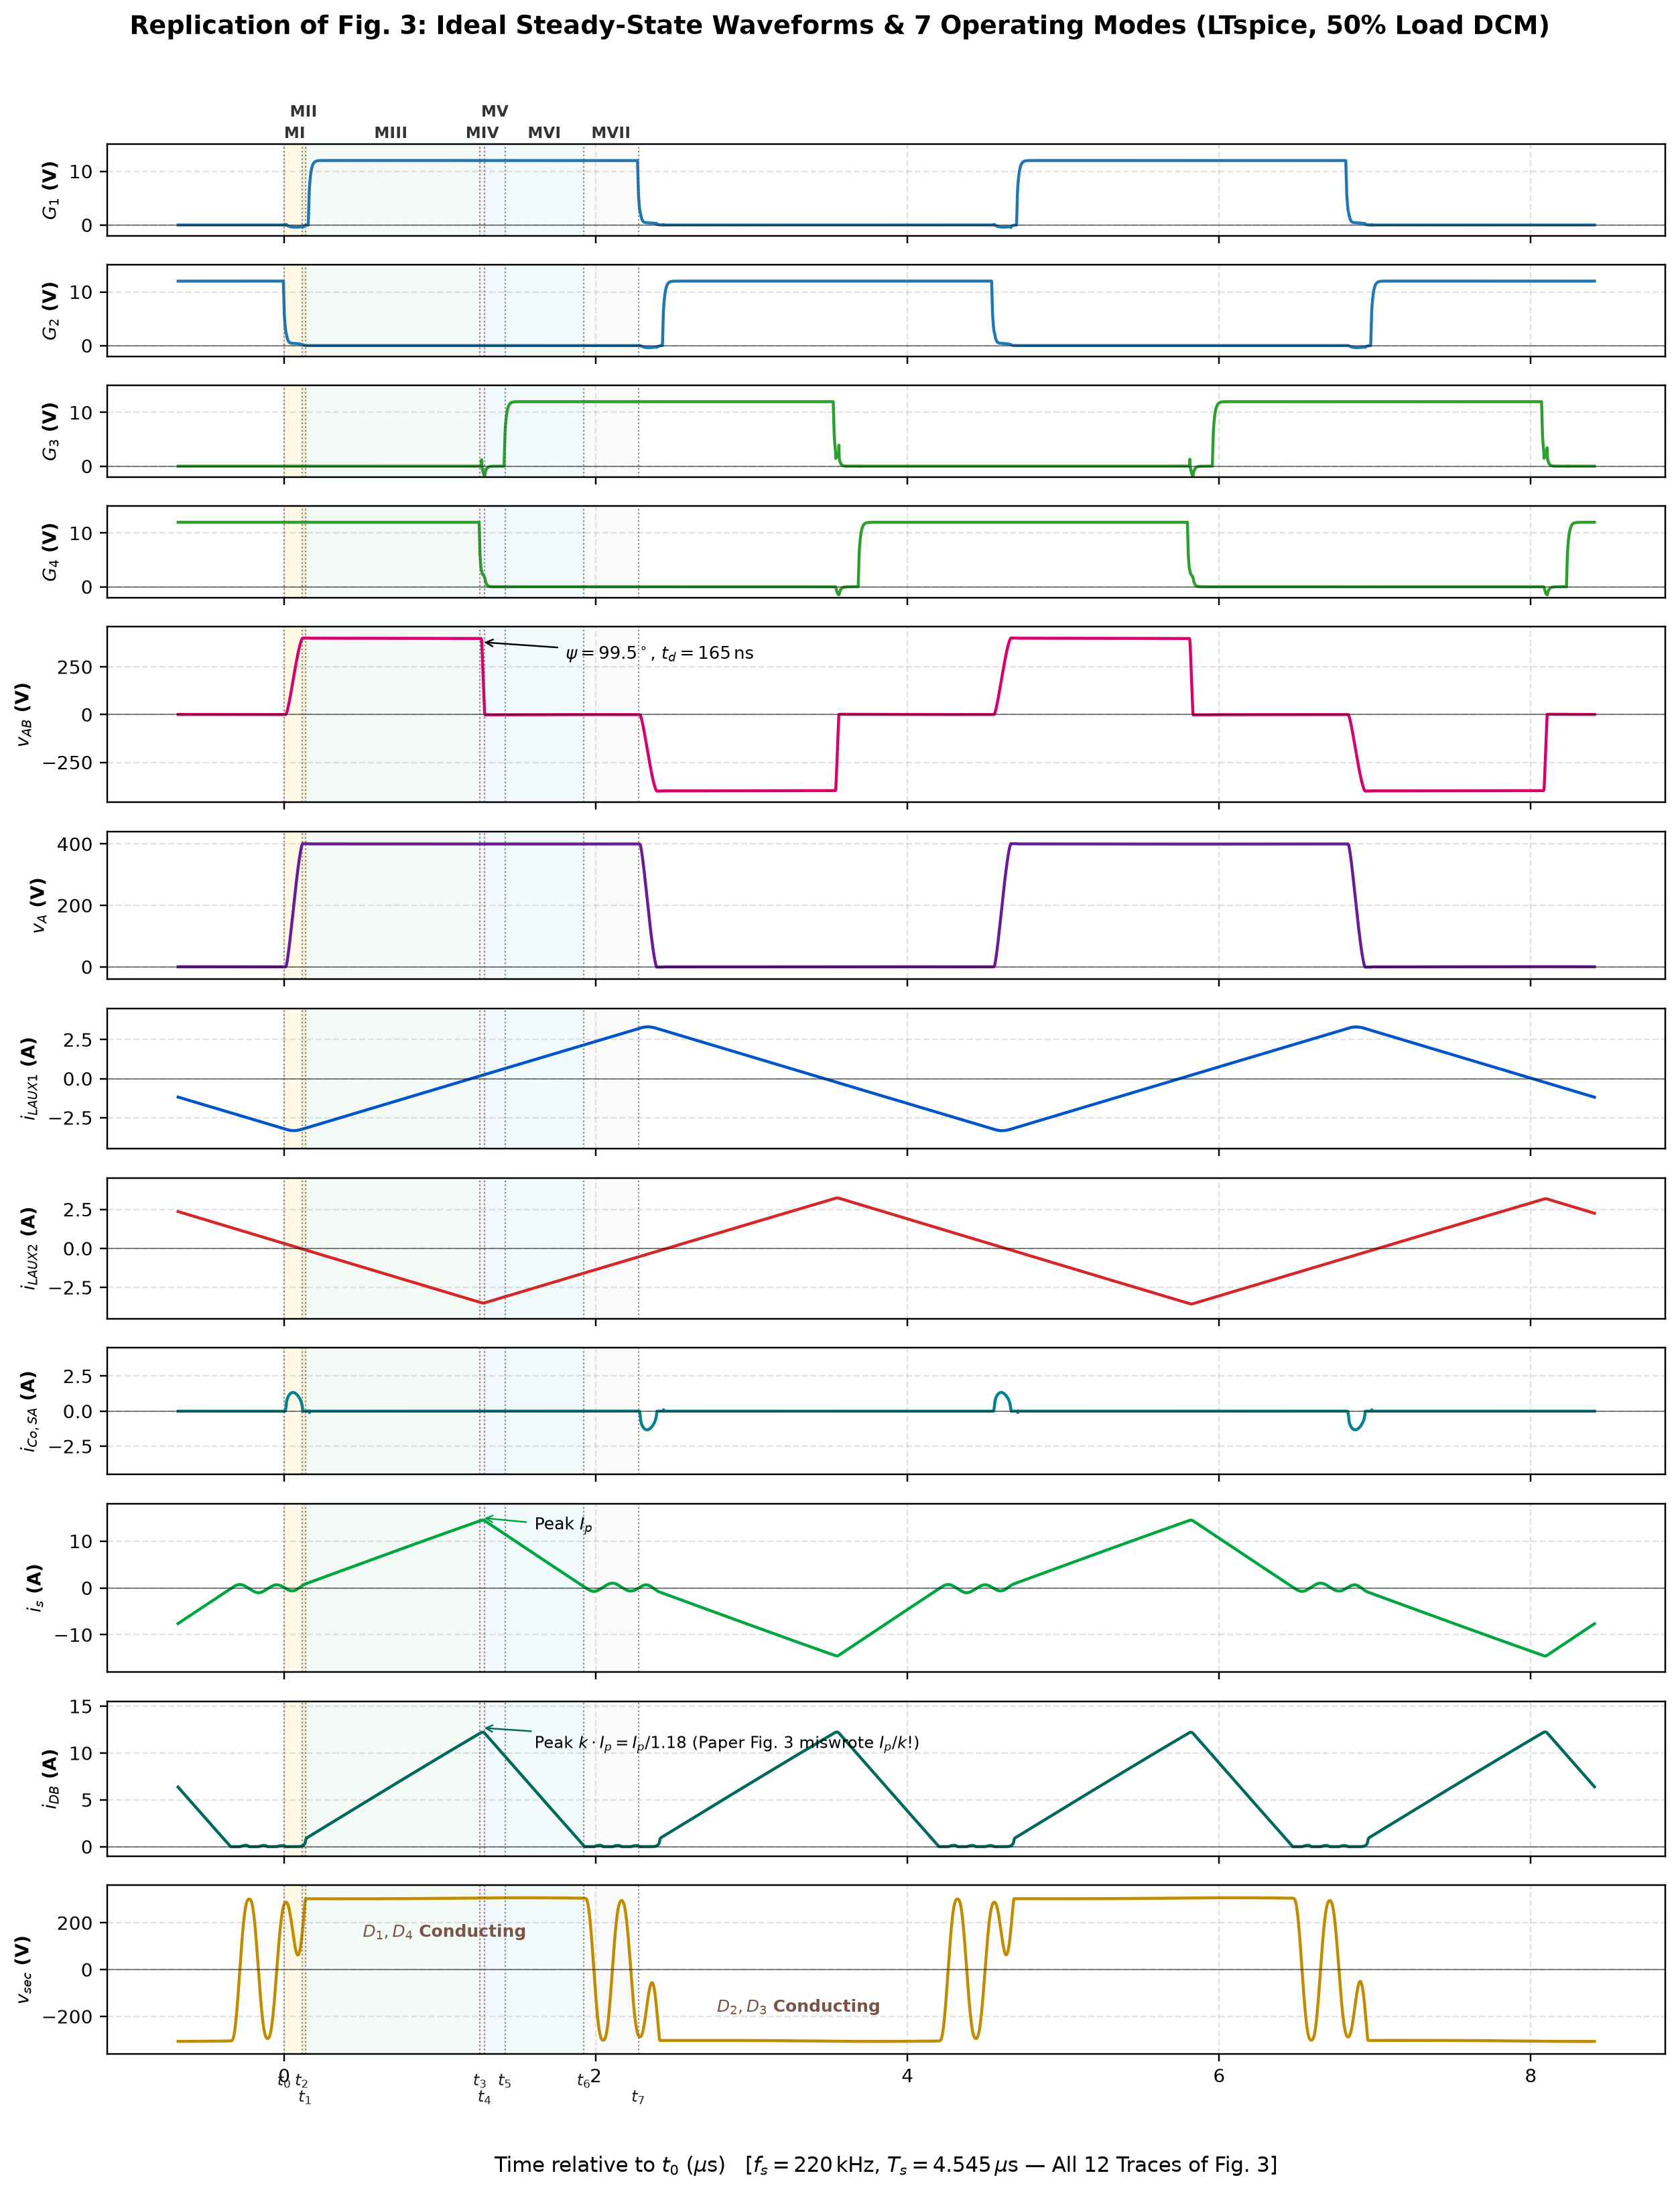
\includegraphics[height=6.55cm,keepaspectratio]{fig03_ideal_waveforms_modes.png}
    \end{column}
    \begin{column}{0.60\textwidth}
      \scriptsize
      In un periodo completo $T_s = 4.545\us$ il convertitore attraversa \textbf{14 modi} (7 nel semiperiodo positivo $t_0\text{--}t_7$, 7 simmetrici nel negativo).

      \vspace*{1.5mm}
      \textbf{\color{PrimaryBlue}Guida alle 12 tracce (dall'alto al basso):}
      \begin{itemize}\setlength{\itemsep}{1.6pt}
        \item \textbf{$G_1, G_2$ (blu) e $G_3, G_4$ (verde)}: comandi gate $0\text{--}12\V$; $G_1, G_2$ anticipano $G_3, G_4$ di $\psi = 99.5^\circ$, con $t_d = 165\ns$ tra switch della stessa gamba.
        \item \textbf{$v_{AB}$ (magenta)}: onda quasi-quadra $\pm 400\V$ con transizioni dolci ZVS.
        \item \textbf{$v_A$ (viola)}: tensione del nodo \emph{leading} ($0$ o $+400\V$, duty 50\%).
        \item \textbf{$i_{LAUX1}$ (blu), $i_{LAUX2}$ (rosso)}: triangolari simmetriche $\pm 3.39\A$, con picchi esattamente centrati sui fronti di commutazione di $v_A$ e $v_B$!
        \item \textbf{$i_{Co,SA}$ (ciano)}: impulsi di carica/scarica di $C_{s1}, C_{s2}$ solo in $t_0\text{--}t_2$.
        \item \textbf{$i_s$ (verde)}: triangolare primaria DCM (picco $I_p = 14.5\A$), seguita dal debole ringing in Modo VII ($t_6\text{--}t_7$).
        \item \textbf{$i_{DB}$ (verde scuro)}: corrente raddrizzata secondaria, picco \textbf{$k I_p = I_p/1.18 = 12.3\A$} (\emph{Fig.\,3 del paper scrive erroneamente $I_p/k$!}).
        \item \textbf{$v_{sec}$ (oro)}: clampata a $\pm 303\V$ durante conduzione di $D_1, D_4$ (o $D_2, D_3$), oscillante in Modo VII.
      \end{itemize}

      \vspace*{1.5mm}
      \begin{formulabox}
        \textbf{Cronologia del semiperiodo positivo ($0 \to 2.273\us$):}\\
        \textbf{M\,I} ($t_0\text{--}t_1$): rampa $v_{AB}$ (diodi OFF) $\to$ \textbf{M\,II} ($t_1\text{--}t_2$): ZVS $S_1$ $\to$ \textbf{M\,III} ($t_2\text{--}t_3$): rampa attiva $t_{on}$ $\to$ \textbf{M\,IV} ($t_3\text{--}t_4$): risonanza \emph{lagging} $\to$ \textbf{M\,V} ($t_4\text{--}t_5$): diodo $D_{FB3}$ $\to$ \textbf{M\,VI} ($t_5\text{--}t_6$): ZVS $S_3$ + ZCS diodi $\to$ \textbf{M\,VII} ($t_6\text{--}t_7$): DCM ($i_s=0$).
      \end{formulabox}
    \end{column}
  \end{columns}
\end{frame}

% --- SLIDE 12 ---
\begin{frame}{Modo I ($t_0 \to t_1$) e Modo II ($t_1 \to t_2$): Transizione Leading Leg e ZVZCS}{Scarica capacitiva tramite $L_{AUX1}$, accensione di $S_1$ e correzione delle Eqs.\,(6)--(8)}
  \begin{columns}[T,onlytextwidth]
    \begin{column}{0.48\textwidth}
      \scriptsize
      \textbf{\color{PrimaryBlue}Modo I ($t_0 \le t \le t_1$) --- Diodi secondari ancora OFF}
      \begin{itemize}\setlength{\itemsep}{1.8pt}
        \item A $t_0$ si spegne $S_2$ ($S_4$ ON, $i_s = 0$). La corrente costante $I_{PA} = 3.39\A$ di $L_{AUX1}$ scarica $C_{s1}$ e carica $C_{s2}$:
          \[
            v_{Cso}(t) = V_{dc} - \frac{I_{PA}}{2C_{so}}(t-t_0), \quad v_{AB}(t) = \frac{I_{PA}}{2C_{so}}(t-t_0) \eqnum{2--3}
          \]
        \item Finch\'e $v_{sec} < V_o+2V_d$, i diodi $D_1\text{--}D_4$ sono OFF: $v_{AB}$ insiste su $L_{seq}+L_M$ (grande!), quindi $i_s$ \`e minuscola:
          \[
            i_s(t) = \frac{1}{L_{seq}+L_M}\!\int_{t_0}^{t}\! v_{AB}\,dt = \frac{I_{PA}(t-t_0)^2}{4(L_{seq}+L_M)C_{so}} \eqnum{1, 4}
          \]
        \item Termina a $t_1$ quando $v_{sec}$ raggiunge $V_o+2V_d$:
          \[
            t_1 = t_0 + \frac{2k(V_o+2V_d)(L_{seq}+L_M)C_{so}}{L_M I_{PA}} \approx t_0 + 99.2\ns \eqnum{5}
          \]
        \item Con $C_{so}=650\pF$, $L_M=1.5\mH$: $i_s(t_1) = \mathbf{8.49\,\text{mA}}$ (trascurabile!).
      \end{itemize}
    \end{column}
    \begin{column}{0.50\textwidth}
      \scriptsize
      \textbf{\color{PrimaryBlue}Modo II ($t_1 \le t \le t_2$) --- Clamping e ZVZCS di $S_1$}
      \begin{itemize}\setlength{\itemsep}{1.8pt}
        \item A $t_1$ i diodi conducono e clampano $v_{sec} = V_o + 2V_d$ ($L_M$ \`e bypassata dalla tensione riflessa $k(V_o+2V_d)$).
        \item $C_{s1}$ termina la scarica fino a $0\V$ all'istante:
          \[
            t_2 = t_0 + \frac{2V_{dc}C_{so}}{I_{PA}} \approx t_0 + 153.3\ns < t_d = 165\ns \eqnum{9}
          \]
        \item A $v_{Cso}=0$ conduce il diodo SiC $D_{FB1}$: $S_1$ si accende a \textbf{tensione nulla (ZVS)} e corrente di carico quasi nulla (\textbf{near-ZCS} $\Rightarrow$ \textbf{ZVZCS})!
      \end{itemize}
      \vspace*{1mm}
      \begin{warnbox}[title={Audit Critico su Eqs.\,(6)--(8) del Paper!}]
        Il paper scrive in Eq.\,(7) $v_{AB}(t)=\frac{I_{PA}}{2C_{so}}(t-t_1)$ dimenticando $v_{AB}(t_1)=k(V_o+2V_d)$ (e integra da $t_0$ in Eq.\,6). Posto $\Delta t = t_2 - t_1$, ottiene:
        \[
          i_{s,\text{paper}}(t_2) = \frac{I_{PA}\,\Delta t^2}{4L_{seq}C_{so}} - \frac{k(V_o+2V_d)\,\Delta t}{L_{seq}} = \mathbf{-0.854\A}
        \]
        Corrente \textbf{negativa} in conduzione diretta! \textbf{Formula fisica corretta:}
        \[
          i_s(t) = i_s(t_1) + \frac{I_{PA}}{4 L_{seq} C_{so}}(t-t_1)^2 \;\Rightarrow\; i_s(t_2) = \mathbf{+0.332\A} > 0
        \]
      \end{warnbox}
    \end{column}
  \end{columns}
\end{frame}

% --- SLIDE 13 ---
\begin{frame}{Modo III ($t_2 \to t_3$): Trasferimento Attivo di Potenza e Fig.\,6}{Rampa lineare in $L_{seq}$ durante $t_{on}$ e confronto con la smagnetizzazione}
  \begin{columns}[T,onlytextwidth]
    \begin{column}{0.45\textwidth}
      \scriptsize
      \textbf{\color{PrimaryBlue}Fisica del Modo III ($t_2 \le t \le t_3$):}
      \begin{itemize}\setlength{\itemsep}{2pt}
        \item $S_1$ e $S_4$ conducono pienamente $\Rightarrow$ $v_{AB}(t) = +V_{dc} = +400\V$.
        \item I diodi secondari clampano $v_{sec} = V_o + 2V_d = 303\V$, riflessa al primario come $k(V_o+2V_d) = 256.8\V$.
        \item Su $L_{seq}=11.8\uH$ insiste una tensione costante positiva:
          \[
            v_{Lseq} = V_{dc} - k(V_o + 2V_d) = +143.2\V
          \]
        \item La corrente $i_s(t)$ sale linearmente fino al picco $I_p$ (Eq.\,10 corretta, includendo $+i_s(t_2)$ omesso dal paper):
          \[
            i_s(t) = i_s(t_2) + \frac{V_{dc} - k(V_o + 2V_d)}{L_{seq}}\,(t - t_2) \eqnum{10}
          \]
          con pendenza $\frac{di_s}{dt} = \mathbf{+12.14\A/\us}$!
        \item Termina a $t_3$ allo spegnimento di $S_4$:
          \[
            t_3 = t_2 + \frac{\psi}{\omega_s} - t_d = t_2 + t_{on} \eqnum{12}
          \]
      \end{itemize}
      \vspace*{1mm}
      \begin{notebox}
        \textbf{Nota su Fig.\,6 e Eq.\,(11):} Fig.\,6 del paper stampa il refuso $V_o - 2V_d$ anzich\'e $V_o + 2V_d$; l'Eq.\,(11) per $I_p$ eredita gli errori dell'Eq.\,(8) e aggiunge un fattore $2$ spurio.
      \end{notebox}
    \end{column}
    \begin{column}{0.53\textwidth}
      \centering
      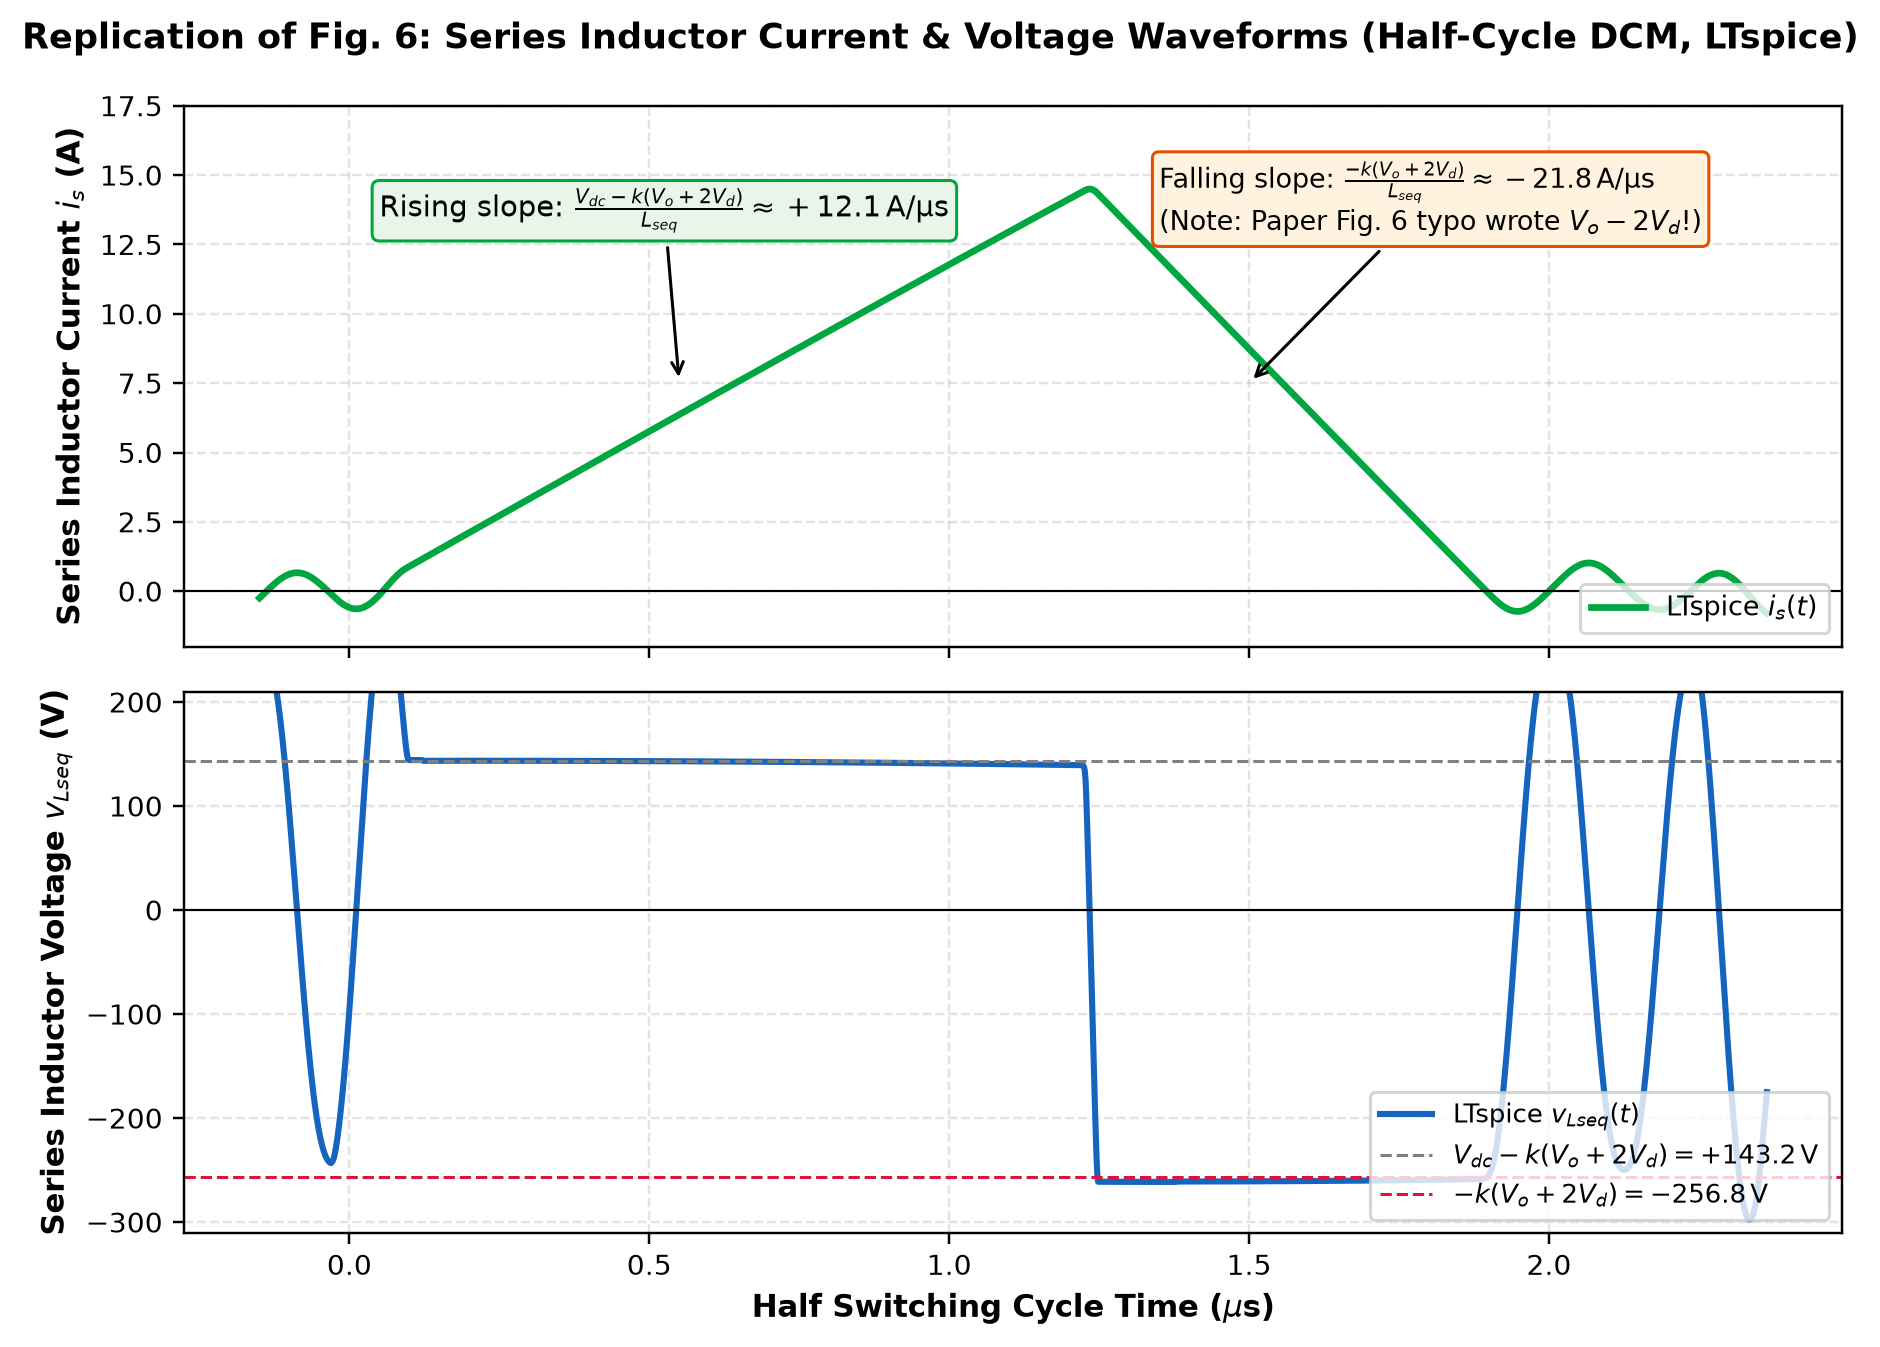
\includegraphics[width=\textwidth,height=5.75cm,keepaspectratio]{fig06_series_inductor_vi.png}\\[-1mm]
      {\tiny\color{MutedGray}Replica LTspice di Fig.\,6: corrente $i_s(t)$ (sopra) e tensione $v_{Lseq}(t)$ (sotto) nel semiperiodo DCM al 50\% di carico: evidenti i due plateau $+143.2\V$ e $-256.8\V$ e il ringing in Modo VII.}
    \end{column}
  \end{columns}
\end{frame}

% --- SLIDE 14 ---
\begin{frame}{Modo IV ($t_3 \to t_4$): Transizione Risonante Lagging Leg e Sottomodi (Fig.\,5)}{Risonanza $L_{seq}$--$2C_{so}$, transizione a due pendenze a bassissimo carico e audit Eqs.\,(13)--(14)}
  \begin{columns}[T,onlytextwidth]
    \begin{column}{0.46\textwidth}
      \scriptsize
      \textbf{\color{PrimaryBlue}Fisica del Modo IV ($t_3 \le t \le t_4$):}
      \begin{itemize}\setlength{\itemsep}{1.5pt}
        \item A $t_3$ si spegne $S_4$ ($S_1$ resta ON). La somma $i_s(t) + I_{PB}$ scarica $C_{s3}$ e carica $C_{s4}$, portando $v_{AB}$ da $+400\V$ a $0\V$.
        \item \textbf{Risonanza $L_{seq}$--$2C_{so}$:}
          $\omega_r = \frac{1}{\sqrt{2C_{so}L_{seq}}} = 8.07\times 10^6\,\text{rad/s}$ ($f_r = \mathbf{1.29\MHz}$).
        \item \textbf{Sottomodi IV-a e IV-b a basso carico (Fig.\,5):}
          \begin{itemize}\setlength{\itemsep}{1pt}
            \item \textbf{10\% carico} ($300\W, I_p=6.6\A$, continua): scarica rapida in $\mathbf{52\ns}$ a singola pendenza.
            \item \textbf{No-load} ($I_p<1.8\A, <50\W$, tratteggiata): $i_s=0$ a $t_{3\text{-}4}<t_4 \Rightarrow$ \textbf{doppia pendenza}: \textbf{IV-a} $-\frac{i_s+I_{PB}}{2C_{so}}$;\; \textbf{IV-b} $-\frac{I_{PB}}{2C_{so}}$ ($I_{PB}$ completa lo ZVS!).
          \end{itemize}
      \end{itemize}
      \vspace*{1.5mm}
      \begin{warnbox}[title={Errore Dimensionale Catastrofico in Eqs.\,(13)--(14)}]
        Il paper scrive $\sin(t/\sqrt{2C_{so}L_{seq}}-t_3)$ (sottrae secondi a radianti!) e in Eq.\,(14) \textbf{divide} per $\sqrt{2C_{so}L_{seq}}$ anzich\'e moltiplicare: il termine coseno vale $\mathbf{2.74\times 10^{14}\A/\text{s}^2}$ invece di $\mathbf{4.20\A}$, e manca il $(-1)$ dell'integrale definito!
      \end{warnbox}
    \end{column}
    \begin{column}{0.52\textwidth}
      \centering
      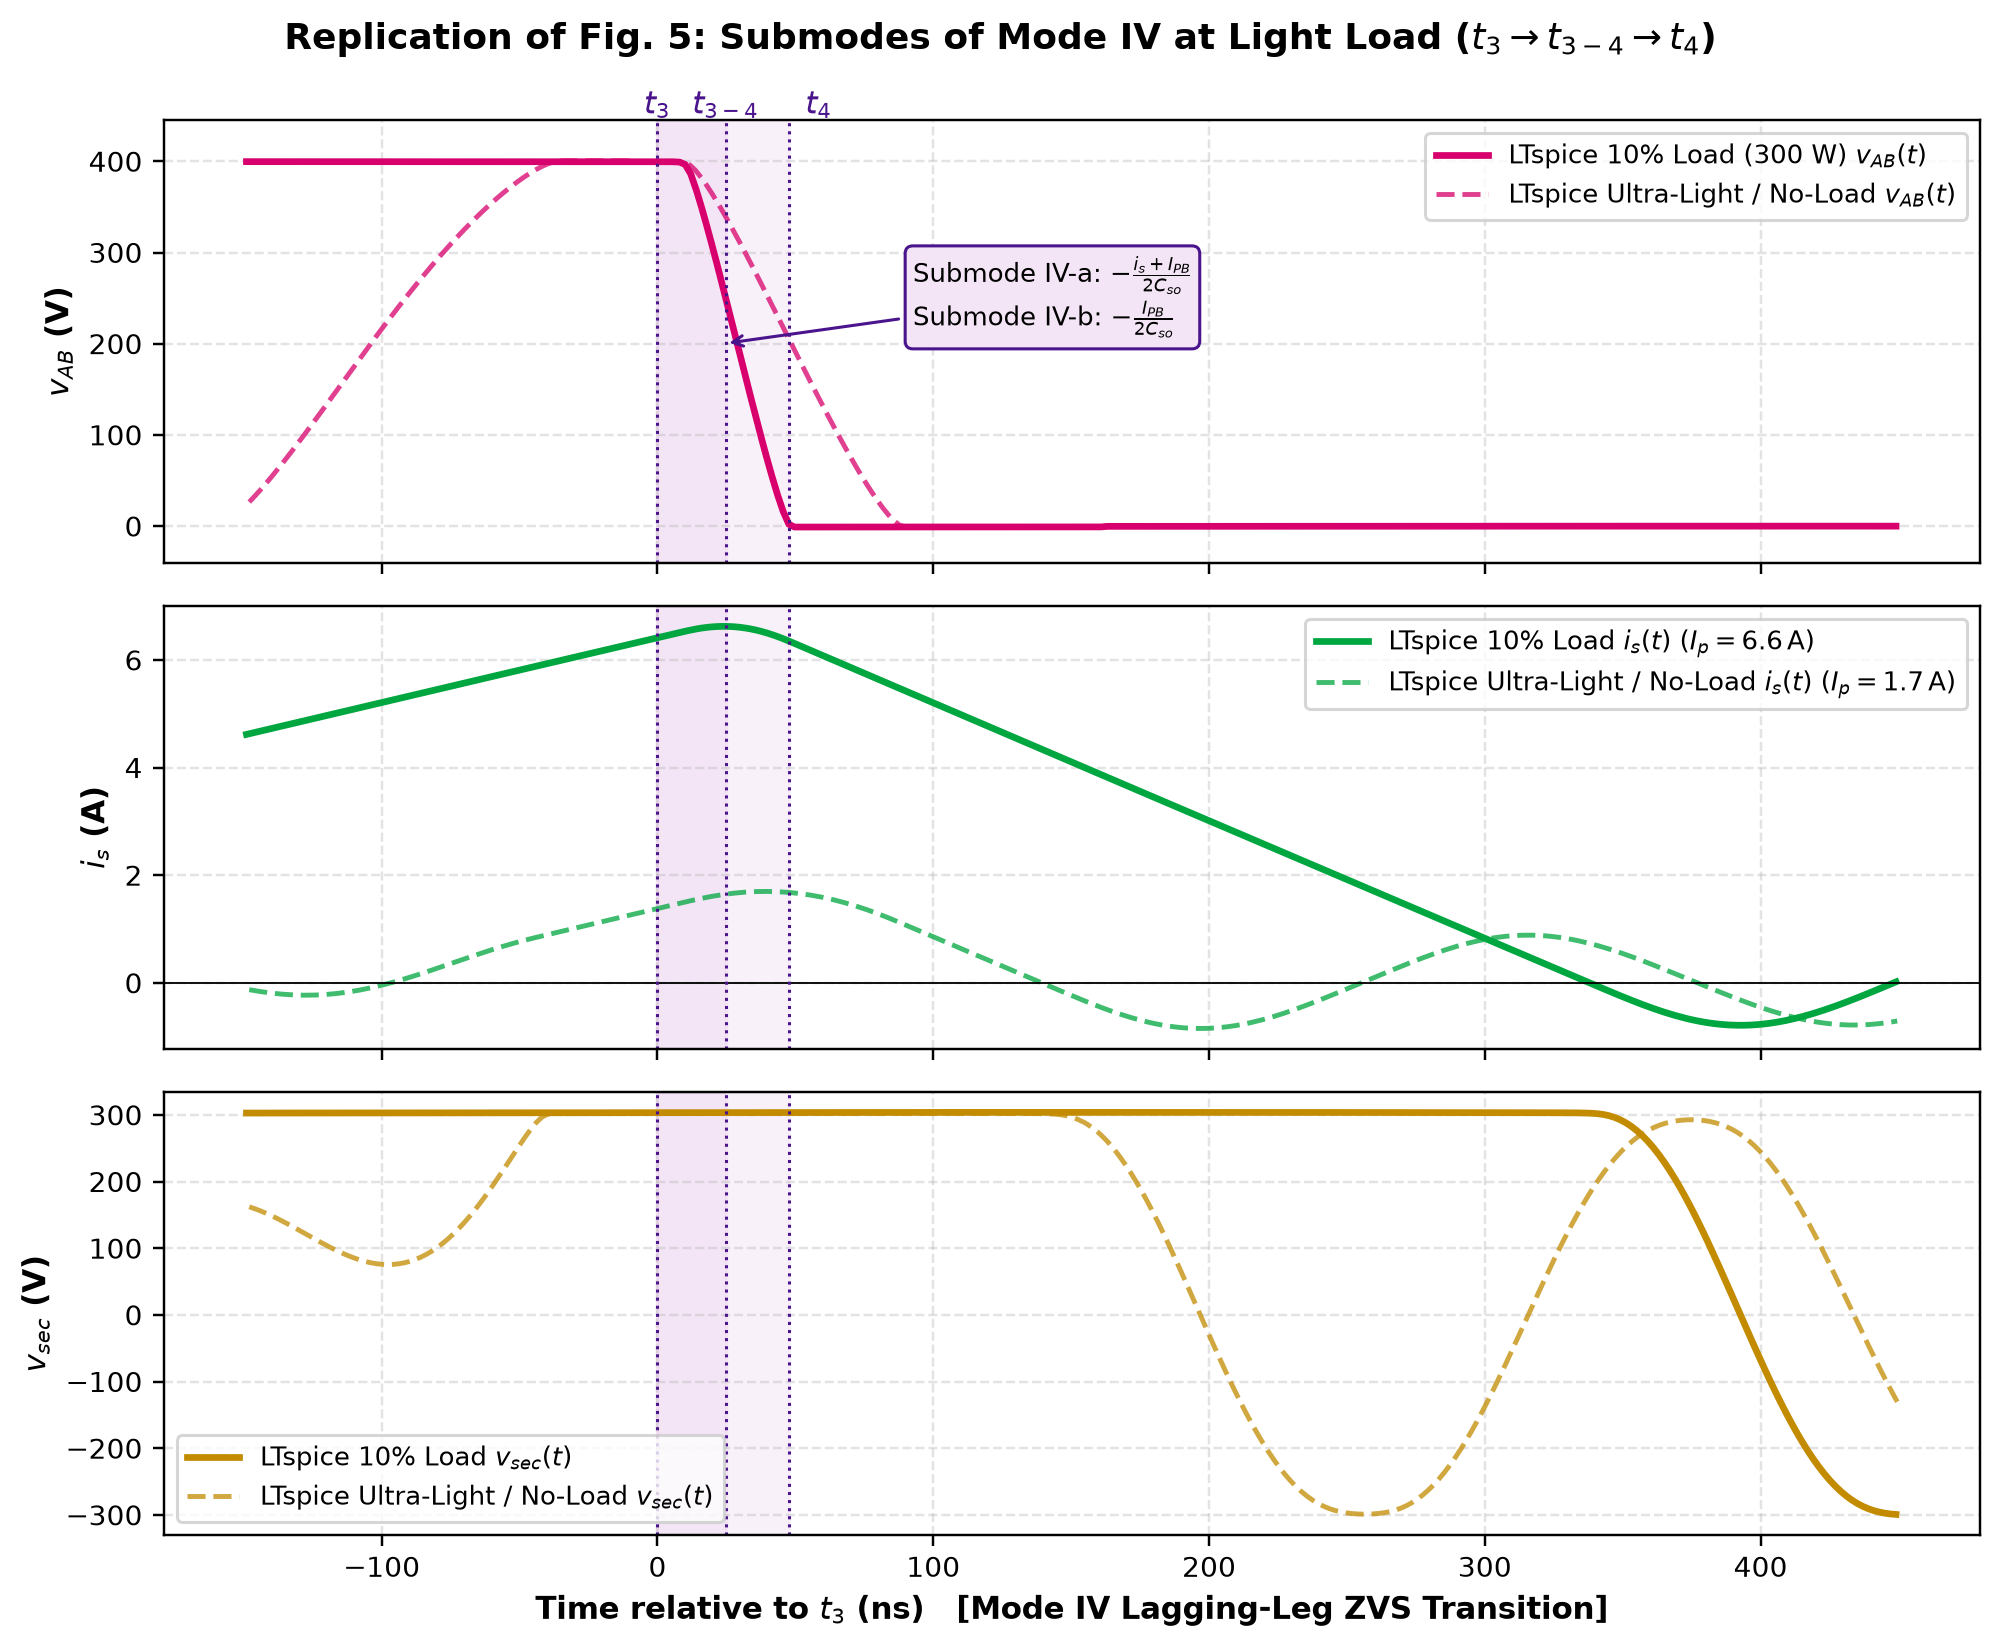
\includegraphics[width=\textwidth,height=5.95cm,keepaspectratio]{fig05_mode4_light_load_submodes.png}\\[-1mm]
      {\tiny\color{MutedGray}Replica LTspice di Fig.\,5: confronto della transizione \emph{lagging} tra 10\% di carico ($I_p=6.6\A$, rapida) e no-load ($I_p=1.7\A$, doppia pendenza IV-a / IV-b).}
    \end{column}
  \end{columns}
\end{frame}

% --- SLIDE 15 ---
\begin{frame}{Modi V, VI e VII ($t_4 \to t_7$): Smagnetizzazione, ZVS, ZCS e Intervallo DCM}{Dalla chiusura del diodo antiparallelo fino all'azzeramento totale della corrente primaria}
  \begin{columns}[T,onlytextwidth]
    \begin{column}{0.32\textwidth}
      \begin{formulabox}[title={Modo V ($t_4 \le t \le t_5$) --- Dead-Time}]
        \begin{itemize}\setlength{\itemsep}{2pt}
          \item A $t_4$ la tensione $v_{AB}$ arriva a $0\V$ ($C_{s3}$ scarico): entra in conduzione il diodo SiC \textbf{$D_{FB3}$} in antiparallelo a $S_3$.
          \item Il secondario \`e ancora clampato a $V_o+2V_d$, quindi su $L_{seq}$ insiste $-k(V_o+2V_d)=-256.8\V$.
          \item Equazione (15) (\textbf{esatta}):
            \[
              i_s(t) = i_s(t_4) - \frac{k(V_o+2V_d)}{L_{seq}}(t-t_4)
            \]
          \item Discesa lineare a $\mathbf{-21.8\A/\us}$; termina a $t_5$ all'arrivo di $G_3$.
        \end{itemize}
      \end{formulabox}
    \end{column}
    \begin{column}{0.32\textwidth}
      \begin{okbox}[title={Modo VI ($t_5 \le t \le t_6$) --- ZVS + ZCS}]
        \begin{itemize}\setlength{\itemsep}{2pt}
          \item A $t_5$ si accende il canale di $S_3$ mentre $D_{FB3}$ conduce ($V_{DS,S3}<0$) $\Rightarrow$ \textbf{ZVS perfetto} sulla \emph{lagging leg}!
          \item $i_s(t)$ prosegue la rampa discendente a $-21.8\A/\us$ cedendo l'energia di $L_{seq}$ all'uscita.
          \item A $t_6$ la corrente $i_s$ arriva a \textbf{zero}: i diodi d'uscita si spengono \textbf{naturalmente in ZCS} senza recupero inverso n\'e spike!
          \item Durata discesa: $t_{off} \approx 0.558\,t_{on}$.
        \end{itemize}
      \end{okbox}
    \end{column}
    \begin{column}{0.32\textwidth}
      \begin{notebox}[title={Modo VII ($t_6 \le t \le t_7$) --- DCM}]
        \begin{itemize}\setlength{\itemsep}{2pt}
          \item $i_s = 0$, tutti i diodi d'uscita $D_1\text{--}D_4$ sono interdetti.
          \item \textbf{Freewheeling azzerato!} Nessuna corrente di carico circola nel primario (solo la piccola $i_{LAUX}$).
          \item $C_f$ sostiene da solo $I_o$ in $L_f$ verso la batteria HV.
          \item Ringing smorzato a $\approx 4.7\MHz$ attorno a $-V_o/2$ (limitato in $[0, -V_o]$).
          \item A $t_7$ si spegne $S_1$ in \textbf{near-ZCS} e inizia il semiperiodo negativo!
        \end{itemize}
      \end{notebox}
    \end{column}
  \end{columns}

  \vspace*{2mm}
  \begin{formulabox}
    \textbf{Riepilogo Soft-Switching in DCM ($0\text{--}75\%$ con $11.8\uH$, o $0\text{--}100\%$ con $8.0\uH$):}\quad
    \textbf{Leading Leg ($S_1, S_2$):} accensione \textbf{ZVZCS} (ZVS da $L_{AUX1}$ + near-ZCS da DCM) e turn-off \textbf{near-ZCS}.\quad
    \textbf{Lagging Leg ($S_3, S_4$):} accensione \textbf{ZVS} (assistito da $I_p + I_{PB}$).\quad
    \textbf{Diodi ($D_1\text{--}D_4$):} turn-off \textbf{ZCS naturale} + clamping rigido a $V_o$.
  \end{formulabox}
\end{frame}

% --- SLIDE 16 ---
\begin{frame}{Quadro Completo di Tutte le Risonanze Presenti nel Convertitore}{Sintesi fisica e quantitativa delle 5 interazioni LC (benefiche, innocue e distruttive)}
  \scriptsize
  \setlength{\tabcolsep}{3.5pt}
  \renewcommand{\arraystretch}{1.18}
  \begin{tabular}{@{}>{\raggedright\arraybackslash}p{2.30cm}>{\raggedright\arraybackslash}p{2.25cm}>{\raggedright\arraybackslash}p{3.05cm}>{\raggedright\arraybackslash}p{6.25cm}@{}}
    \toprule
    \textbf{Risonanza} & \textbf{Elementi LC} & \textbf{Frequenza / Formula} & \textbf{Effetto fisico e impatto progettuale} \\
    \midrule
    \textbf{1. Transizione Modo IV} (\emph{lagging}) & $L_{seq}$ ($11.8\uH$) $\leftrightarrow$ $2C_{so}$ ($1.3\nF$) & $f_{r,\text{IV}} = \dfrac{1}{2\pi\sqrt{2C_{so}L_{seq}}}$\newline$\approx \mathbf{1.29\MHz}$ & \textbf{\color{GoodGreen}Benefica:} l'energia di $L_{seq}$ assiste $I_{PB}$ nello scaricare rapidamente $C_{s3}/C_{s4}$ in $\sim 50\ns$ garantendo ZVS sulla \emph{lagging leg}. \\
    \textbf{2. Ringing Modo VII} (DCM) & $L_{seq}/k^2$ ($16.4\uH$) $\leftrightarrow$ $C_w + C_{j,\text{eq}}$ ($\approx 70\pF$) & $f_{\text{ring}} = \dfrac{1}{2\pi\sqrt{(L_{seq}/k^2)C_{\text{par}}}}$\newline$\approx \mathbf{4.7\MHz}$ & \textbf{\color{AccentBlue}Innocua:} visibile in Figg.\,15--19 sui diodi centrata a $-V_o/2$; oscilla smorzata \emph{strettamente dentro} $[0, -V_o]$ senza mai eccedere $V_o$! \\
    \textbf{3. Blocco DC primario} & $L_{seq}$ ($11.8\uH$) $\leftrightarrow$ $C_B$ ($22\uF$) & $f_{r,CB} = \dfrac{1}{2\pi\sqrt{L_{seq}C_B}}$\newline$\approx \mathbf{9.9\kHz}$ & \textbf{\color{GoodGreen}Progettata $\ll f_s$:} oltre una decade sotto $220\kHz$, cos\`i $C_B$ blocca la DC senza introdurre sfasamenti o risonanze a $f_s$. \\
    \textbf{4. Boost capacitivo in CCM} & $L_{seq}$ ($11.8\uH$) $\leftrightarrow$ $C_f/k^2$ ($1.39\uF$) & $f_{r,Cf} = \dfrac{1}{2\pi\sqrt{L_{seq}C_f/k^2}}$\newline$\approx \mathbf{39.3\kHz}$ & \textbf{\color{WarnAmber}Effetto secondario in CCM:} la piccola reattanza serie di $C_f$ compensa parzialmente $L_{seq}$, elevando $P_{\max}$ a 300\,V da $2919\W$ (induttivo puro) a $3003\W$! \\
    \textbf{5. Spike PSFB convenzionale} & $L_{leak}$ ($1.8\uH$) $\leftrightarrow$ $C_w+C_j$ + $Q_{rr}$ & Eccitata dallo scontro $L_{leak}$--$L_f$ & \textbf{\color{AlertRed}Distruttiva (solo nel convenzionale):} genera picchi fino a \textbf{961\,V}, fortissima EMI e perdite di snubber. \textbf{Assente nella topologia proposta!} \\
    \bottomrule
  \end{tabular}
\end{frame}

% ==============================================================================
% SEZIONE 4: ANALISI STAZIONARIA E GUADAGNO DI TENSIONE
% ==============================================================================
\section{4. Analisi Stazionaria e Guadagno}

% --- SLIDE 17 ---
\begin{frame}{Analisi Stazionaria: Corrente Media $I$ e Guadagno $g_v(\psi, R_e)$ (Eqs.\,16--19)}{Derivazione passo-passo in DCM e correzione dei 2 errori gravi del paper}
  \begin{columns}[T,onlytextwidth]
    \begin{column}{0.48\textwidth}
      \scriptsize
      \textbf{\color{PrimaryBlue}Ipotesi semplificative (Sezione III del paper):}
      \begin{enumerate}\setlength{\itemsep}{1pt}
        \item Convertitore ideale senza perdite ($P_{in} = P_o$, ESR nulle).
        \item Energia trasferita nei Modi I--II trascurabile ($i_s \approx 0$).
        \item Variazione di $i_s$ nel breve Modo IV trascurabile; $L_M \to \infty$.
        \item Ripple di tensione su $C_f$ piccolo rispetto a $V_o$.
      \end{enumerate}

      \vspace*{2mm}
      \textbf{\color{PrimaryBlue}Passo 1 --- Corrente media primaria raddrizzata $I$:}
      \begin{itemize}\setlength{\itemsep}{1.2pt}
        \item Picco triangolo: $I_p = \frac{V_{dc}-kV_o}{L_{seq}}\,t_{on}$ con $t_{on}=\frac{\psi}{\omega_s}-t_d$.
        \item Base triangolo: $t_{on}+t_{off} = t_{on}\,\frac{V_{dc}}{kV_o}$.
        \item Media su $T_s/2$: area $\frac{1}{2}I_p(t_{on}+t_{off})$ divisa per $\frac{T_s}{2}$ $\Rightarrow$ i fattori $\frac{1}{2}$ si elidono!
      \end{itemize}
      \begin{formulabox}[title={Eq.\,(16) Corretta (nel paper fattore $2/T_s$ errato!)}]
        \[
          I = \frac{\mathbf{1}}{T_s}\left(\frac{\psi}{\omega_s}-t_d\right)^2\!\left(\frac{V_{dc}}{kV_o}\right)\!\left(\frac{V_{dc}-kV_o}{L_{seq}}\right)
        \]
      \end{formulabox}
    \end{column}
    \begin{column}{0.50\textwidth}
      \scriptsize
      \textbf{\color{PrimaryBlue}Passo 2 --- Bilancio di potenza (Eqs.\,17 e 19):}
      \[
        k \cdot I \cdot V_o = V_{BAT}\cdot I_{BAT} = \frac{V_o^2}{R_e}, \qquad R_e = \frac{V_{BAT}}{I_{BAT}}
      \]
      Sostituendo $I$ si ottiene l'equazione quadratica in $g_v = V_o/V_{dc}$:
      \[
        \frac{T_s L_{seq}}{R_e t_{on}^2}\,g_v^2 + k\,g_v - 1 = 0
      \]

      \begin{okbox}[title={Eq.\,(18) Fisicamente Corretta (valida solo in DCM!)}]
        \[
          g_v = \frac{V_o}{V_{dc}} = \frac{2}{k + \sqrt{k^2 + \dfrac{4\,\mathbf{T_s}\,L_{seq}}{R_e \bigl(\frac{\psi}{\omega_s} - t_d\bigr)^2}}}
        \]
      \end{okbox}
      \vspace*{1mm}
      \begin{warnbox}[title={Errore Dimensionale Fatale in Eq.\,(18) del Paper!}]
        Il paper stampa $T_s$ al \textbf{denominatore}: $\frac{4 L_{seq}}{\mathbf{T_s}\,R_e\,t_{on}^2}$ ha dimensioni $[\text{s}^{-2}]$ (non adimensionale!). Valutata a $\psi=90^\circ, R_e=30\Ohm$, d\`a $g_v = \mathbf{3.86\times 10^{-6}}$ (praticamente zero)!\\
        \textbf{Limite DCM:} valida solo finch\'e $t_{on} \le \frac{kV_o}{V_{dc}}\frac{T_s}{2}$; oltre entra in \textbf{CCM} e $g_v$ satura!
      \end{warnbox}
    \end{column}
  \end{columns}
\end{frame}

% --- SLIDE 18 ---
\begin{frame}{Mappa del Guadagno $g_v(\psi, R_e)$: 84 Simulazioni LTspice vs.\ Fig.\,7}{Verifica sperimentale completa e scoperta dell'errore $4\times$ nella curva plottata del paper}
  \centering
  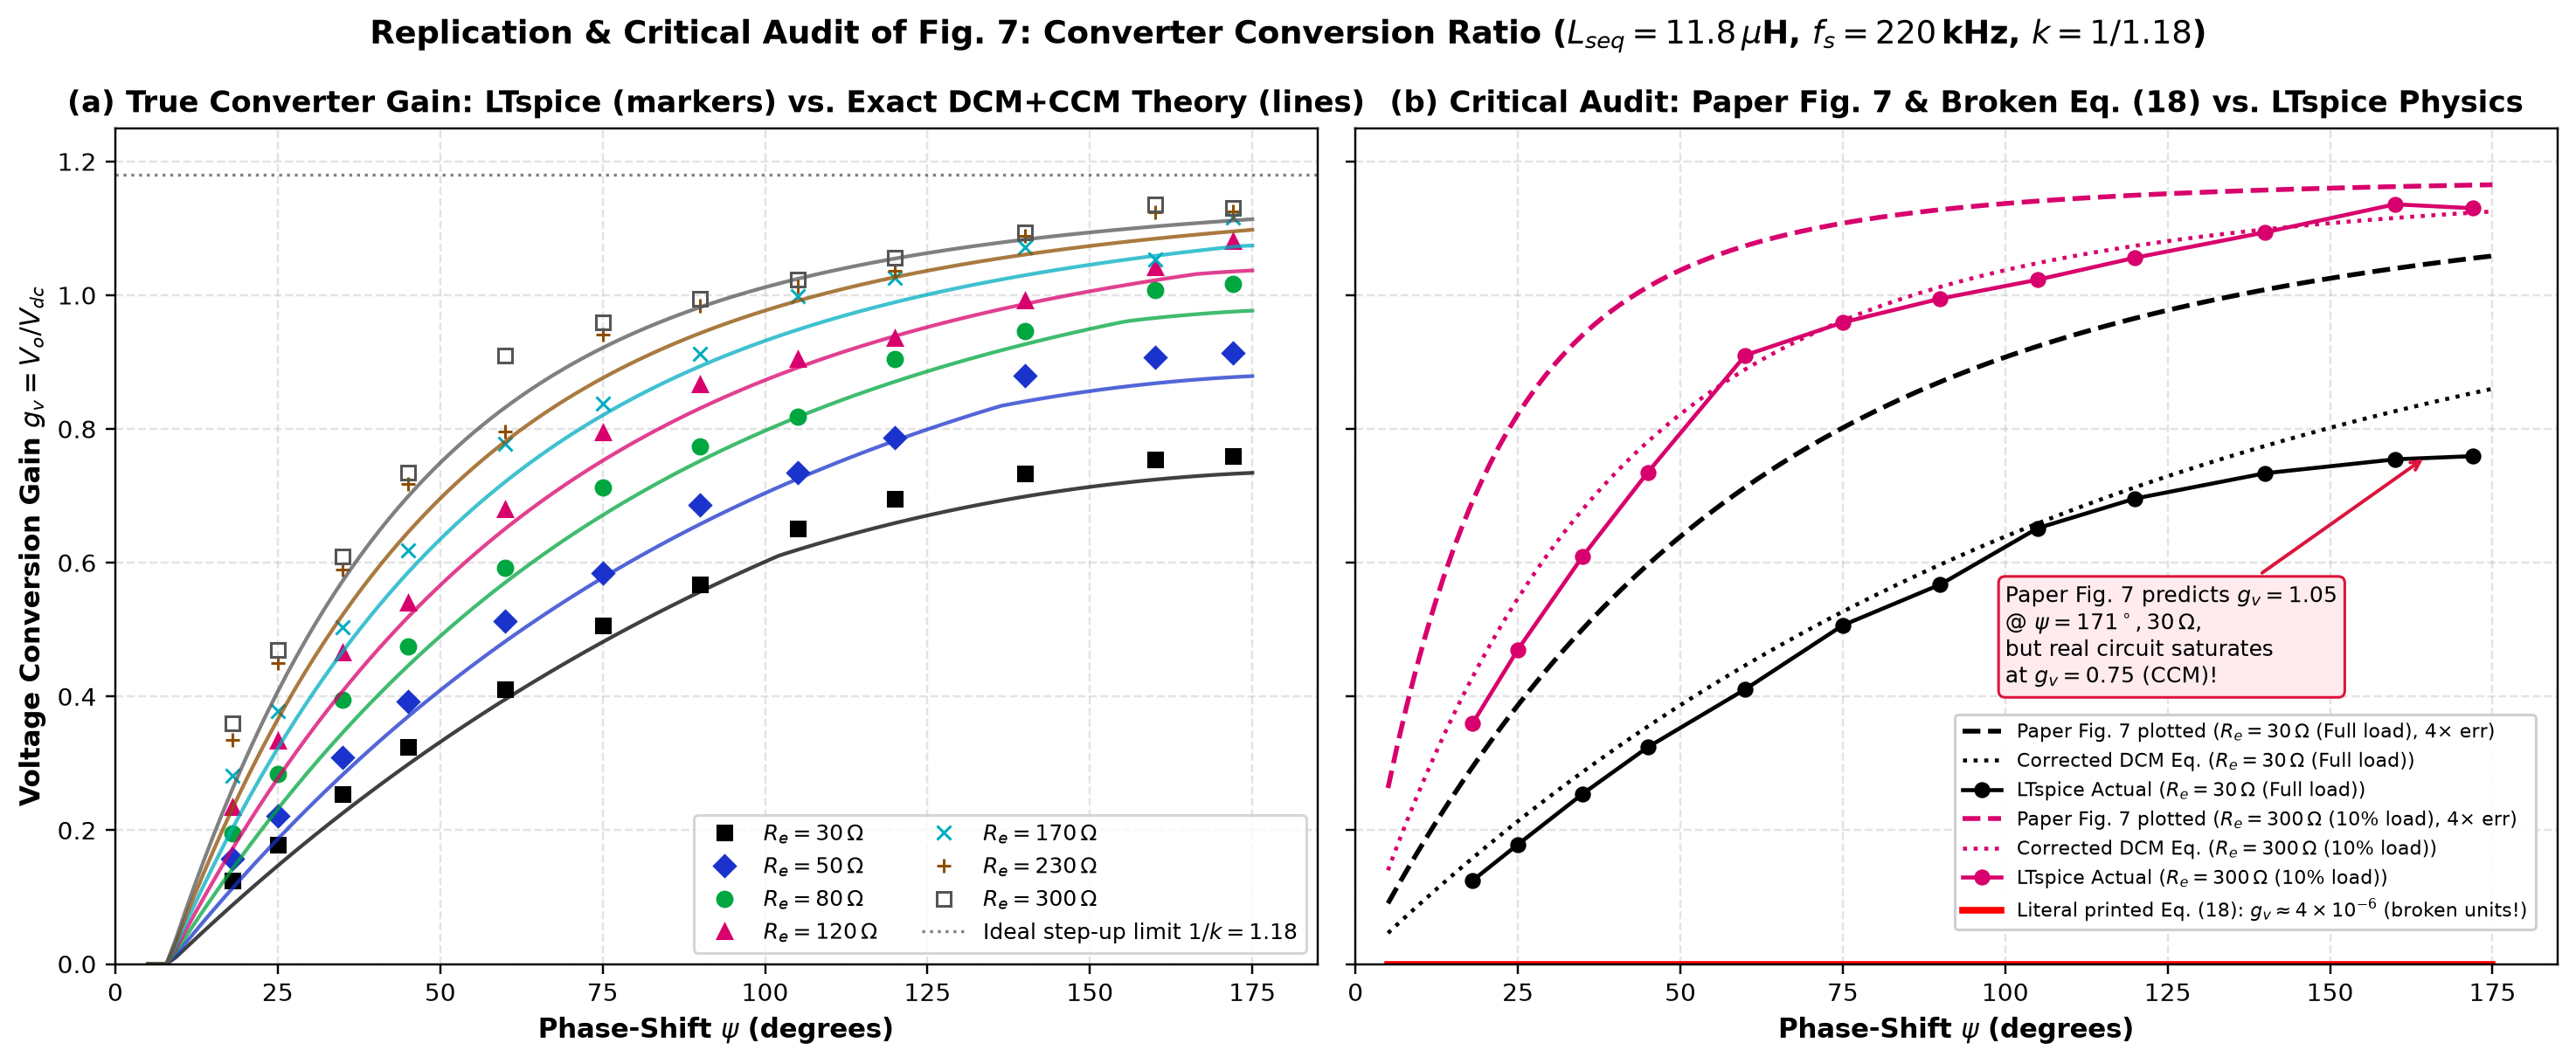
\includegraphics[width=0.92\textwidth,height=4.05cm,keepaspectratio]{fig07_converter_gain_comparison.png}

  \vspace*{1.5mm}
  \begin{columns}[T,onlytextwidth]
    \begin{column}{0.49\textwidth}
      \begin{okbox}[title={Pannello (a): LTspice (84 punti) vs.\ Teoria Esatta DCM+CCM}]
        \begin{itemize}\setlength{\itemsep}{1.2pt}
          \item Sweep 2D in LTspice (\texttt{03\_proposed\_gain\_sweep\_fig7.asc}): $7\,R_e \in [30,300]\Ohm \times 12\,\psi \in [18^\circ,172^\circ]$.
          \item Accordo eccellente con il modello analitico esatto DCM+CCM!
          \item A basso carico ($R_e=300\Ohm$) $g_v$ cresce rapidamente verso $1/k = 1.18$; a pieno carico ($R_e=30\Ohm$) satura in CCM a \textbf{$g_v = 0.759$}.
        \end{itemize}
      \end{okbox}
    \end{column}
    \begin{column}{0.49\textwidth}
      \begin{warnbox}[title={Pannello (b): Scoperta Critica su Fig.\,7 del Paper!}]
        \begin{itemize}\setlength{\itemsep}{1.2pt}
          \item L'Eq.\,(18) stampata (linea rossa) giace a zero ($4\times 10^{-6}$).
          \item Il fit dei pixel di Fig.\,7 dimostra che il grafico usa $C=L_{seq}f_s=2.60\Ohm$, cio\`e \textbf{$4\times$ troppo piccolo} rispetto a $4L_{seq}f_s=10.38\Ohm$ (come usare $\psi/180^\circ$ invece di $\psi/360^\circ$!).
          \item Predice $g_v=1.05$ a $30\Ohm, 171^\circ$ (reale: $0.75$) e $\psi\approx 45^\circ$ al 50\% (contraddicendo Fig.\,18 dello stesso paper: $\psi\approx 95\text{--}100^\circ$!).
        \end{itemize}
      \end{warnbox}
    \end{column}
  \end{columns}
\end{frame}

% ==============================================================================
% SEZIONE 5: PROCEDURA DI PROGETTO DEI COMPONENTI CHIAVE
% ==============================================================================
\section{5. Progetto Componenti}

% --- SLIDE 19 ---
\begin{frame}{Progetto del Circuito Ausiliario Simmetrico ($L_{AUX1}, L_{AUX2}, t_d$ --- Fig.\,8)}{Derivazione Eqs.\,(20)--(24), verifica simmetria in LTspice e nota critica su $t_d$}
  \begin{columns}[T,onlytextwidth]
    \begin{column}{0.46\textwidth}
      \scriptsize
      \textbf{\color{PrimaryBlue}Analisi del ramo ausiliario ($V_{\text{mid}} = V_{dc}/2 = 200\V$):}
      \begin{itemize}\setlength{\itemsep}{1.8pt}
        \item Su $L_{AUX1}$ insiste l'onda quadra $\pm V_{dc}/2$ per $T_s/2$. Corrente triangolare di picco \textbf{indipendente dal carico} ($I_{PA}=I_{PB}$, Eq.\,20 \textbf{corretta}):
          \[
            I_{PA} = \frac{V_{dc}}{8 L_{AUX} f_s} = \frac{400}{8\cdot 67\uH\cdot 220\kHz} = \mathbf{3.39\A} \eqnum{20}
          \]
          \[
            I_{AUX,\text{rms}} = \frac{I_{PA}}{\sqrt{3}} = \mathbf{1.96\A} \;\; (\text{Tab.\,II rating: } 2\A_{\text{rms}})
          \]
        \item Bilancio energetico del paper (Eqs.\,21--24):
          \[
            E_{AUX}=\tfrac{1}{2}L_{AUX}I_{PA}^2 = E_{Cso}=C_{so}V_{dc}^2 \eqnum{21--22}
          \]
          \[
            L_{AUX}=\frac{1}{128 C_{so} f_s^2} \eqnum{23}, \qquad t_d = \frac{2 C_{so} V_{dc}}{I_{PA}} \eqnum{24}
          \]
      \end{itemize}
      \vspace*{1mm}
      \begin{warnbox}[title={Nota Critica su Eqs.\,(23)--(24) vs.\ Prototipo Reale}]
        Combinando (20)+(23)+(24) si ottiene identicamente $t_d = T_s/8 = \mathbf{568.2\ns}$ ($45^\circ$!) e $C_{so}=2.41\nF$ ($3.5\times$ del reale). Con la capacit\`a fisica reale ($C_{so}\approx 550\text{--}650\pF$), il tempo di carica/scarica a vuoto \`e $t_r = \frac{2C_{so}V_{dc}}{I_{PA}} \approx \mathbf{130\text{--}153\ns} < t_d = \mathbf{165\ns}$ $\Rightarrow$ \textbf{ZVS garantito fino allo 0\%}!
      \end{warnbox}
    \end{column}
    \begin{column}{0.52\textwidth}
      \centering
      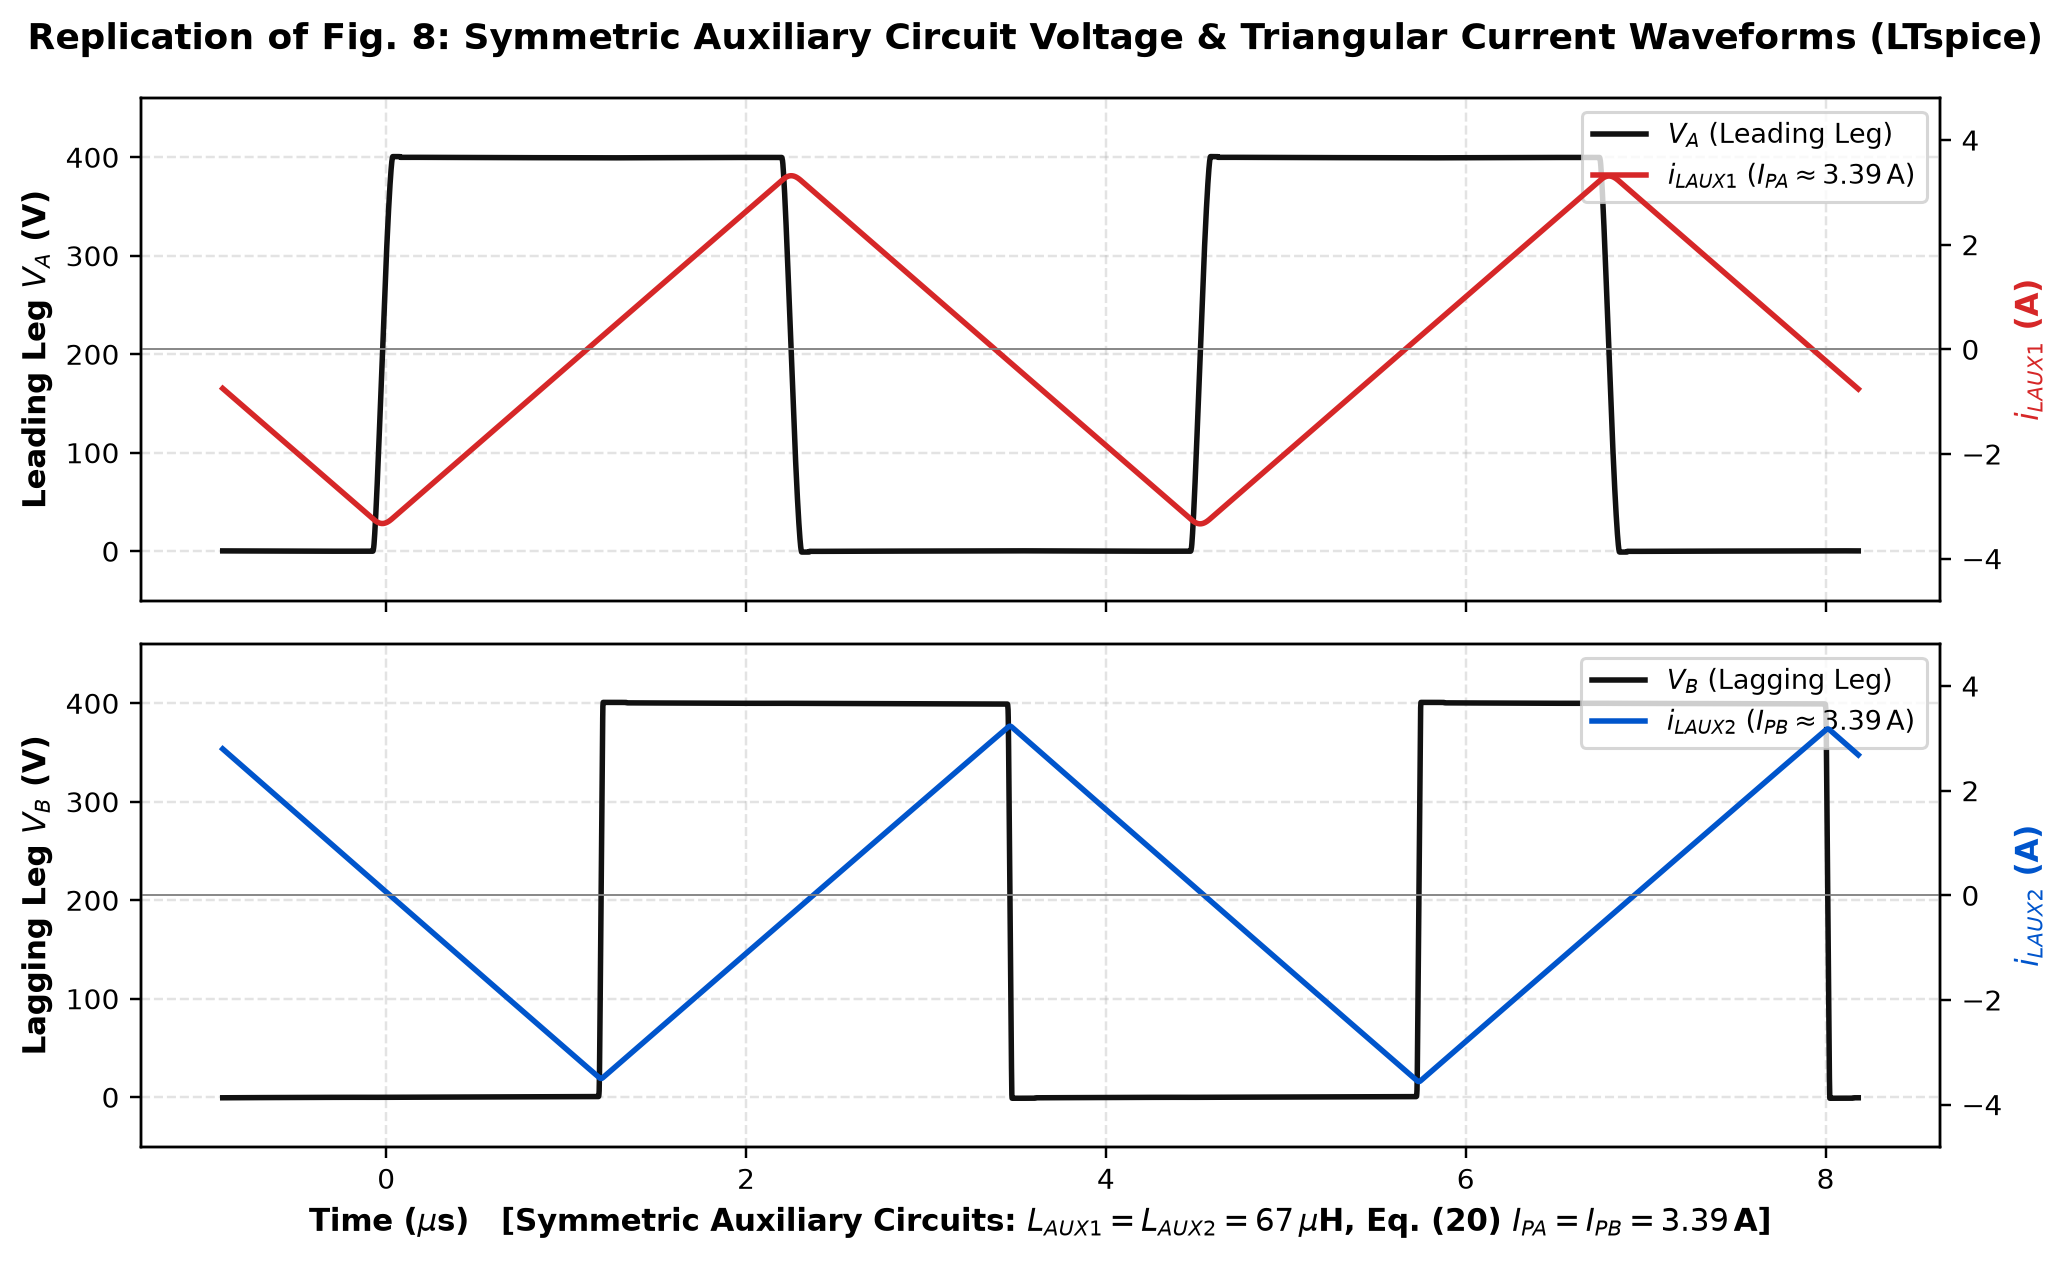
\includegraphics[width=\textwidth,height=4.85cm,keepaspectratio]{fig08_auxiliary_circuit_waveforms.png}\\[-1mm]
      {\tiny\color{MutedGray}Replica LTspice di Fig.\,8: tensioni di gamba $V_A, V_B$ e correnti triangolari simmetriche $i_{LAUX1}, i_{LAUX2}$.}
      \vspace*{1.5mm}
      \begin{okbox}
        \textbf{Lettura del grafico:} i picchi $\pm 3.39\A$ di $i_{LAUX1}$ (rosso) e $i_{LAUX2}$ (blu) coincidono esattamente con i fronti di commutazione di $V_A$ e $V_B$, agendo da generatori di corrente costante durante il tempo morto!
      \end{okbox}
    \end{column}
  \end{columns}
\end{frame}

% --- SLIDE 20 ---
\begin{frame}{Progetto dell'Induttore Serie $L_{seq}$ in Critical Conduction Mode (Fig.\,9)}{Derivazione esatta BCM (Eqs.\,25--26) e confronto tra $11.8\uH$ e $8.0\uH$ in LTspice}
  \centering
  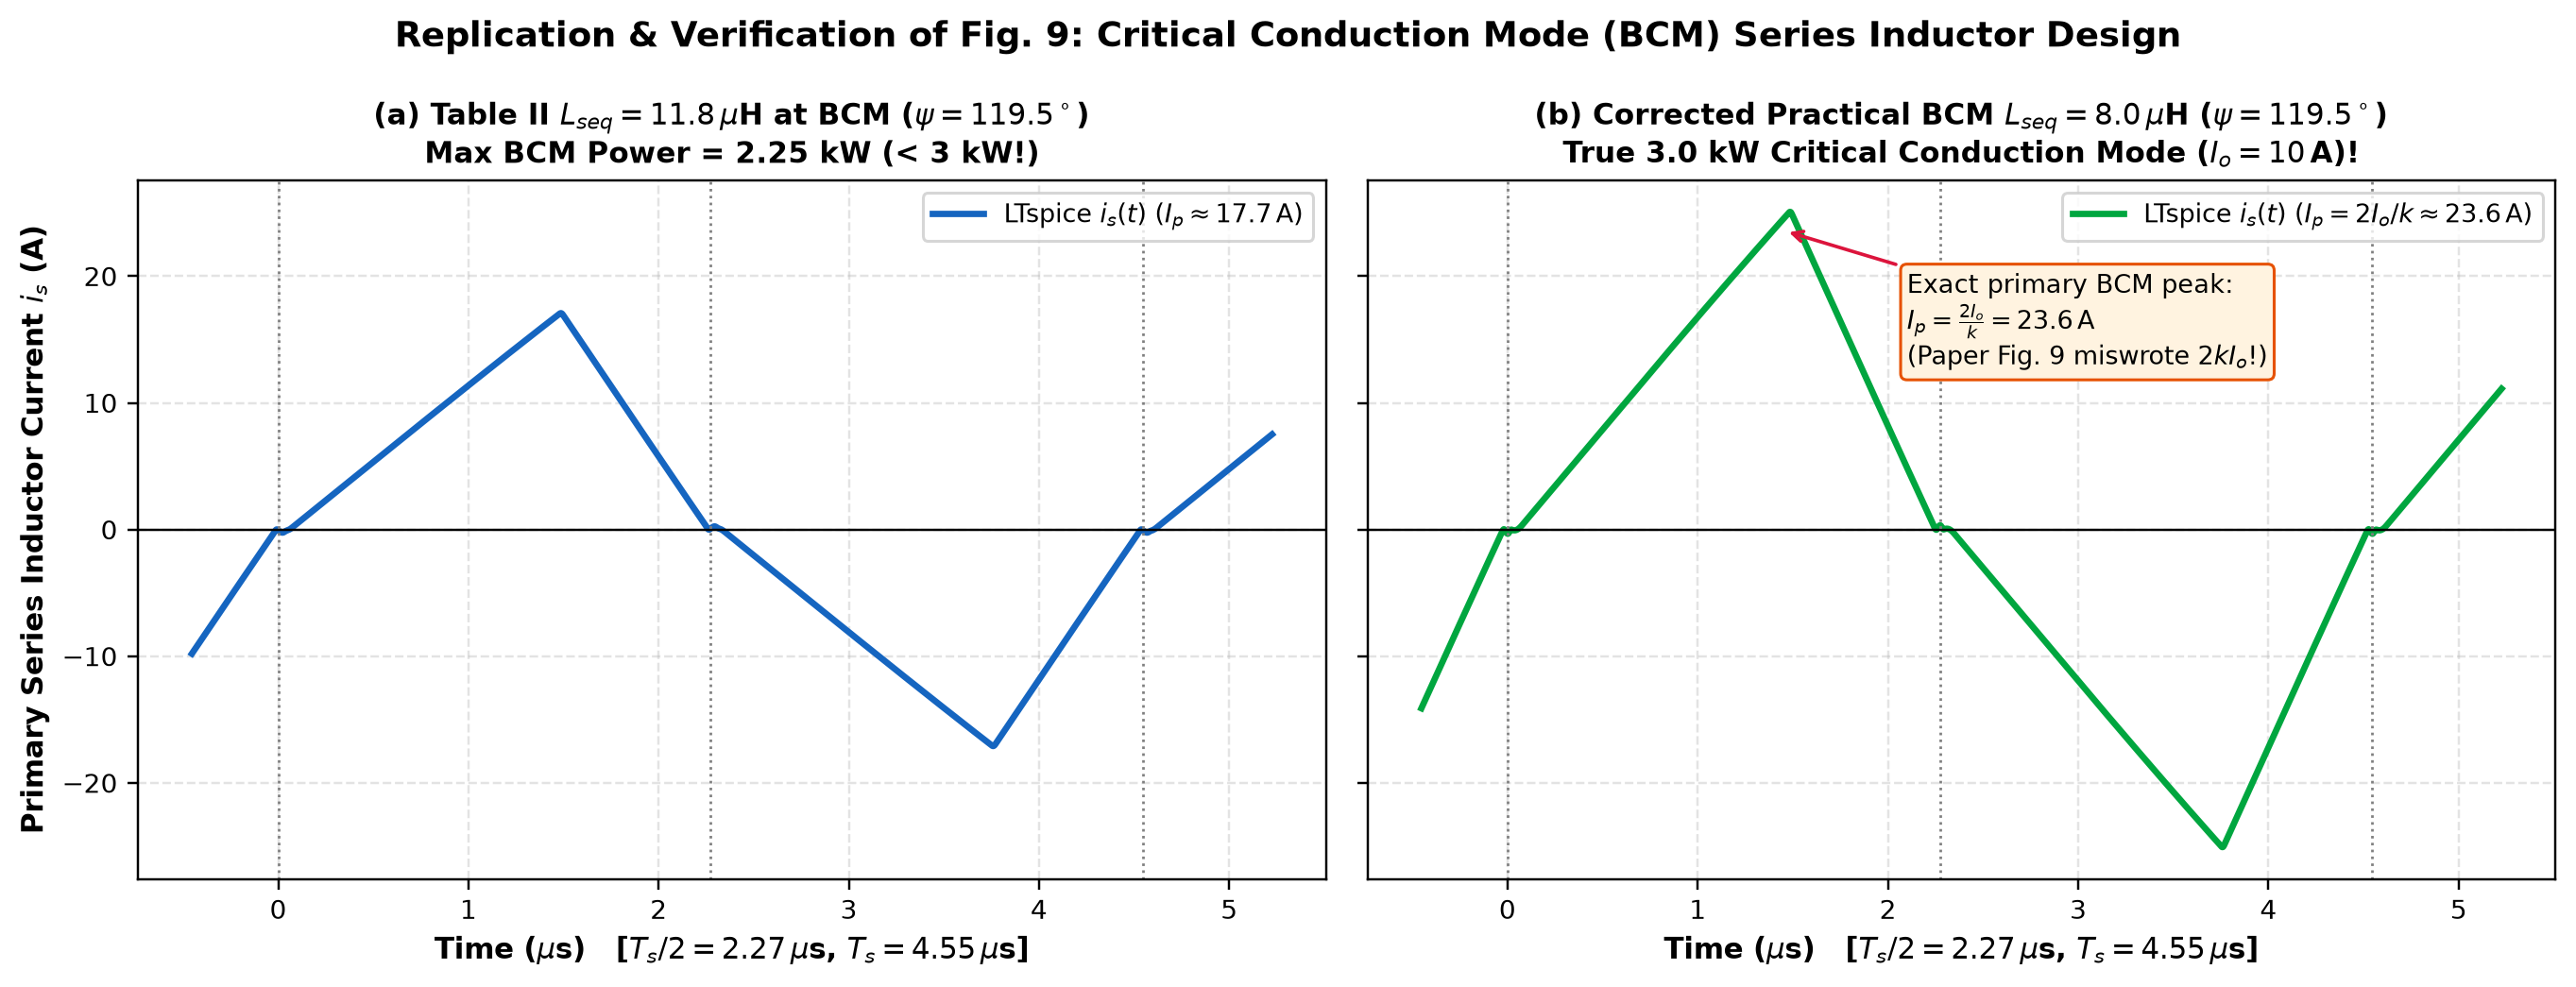
\includegraphics[width=0.92\textwidth,height=3.20cm,keepaspectratio]{fig09_critical_conduction_mode.png}

  \vspace*{1.5mm}
  \begin{columns}[T,onlytextwidth]
    \begin{column}{0.51\textwidth}
      \begin{okbox}[title={Derivazione Fisica Corretta in BCM a $P_{o,\max} = 3\kW$}]
        Al limite BCM ($t_{on}+t_{off}=T_s/2$), si ha $t_{on}=\frac{kV_o}{V_{dc}}\frac{T_s}{2}$. Poich\'e il trasformatore \`e elevatore ($k=1/1.18$), la corrente media primaria \`e $I_o/k$, quindi il picco primario \`e \textbf{$I_p = 2I_o/k = 23.6\A$} (\emph{Fig.\,9 del paper inverte $k$ scrivendo $2kI_o$!}). Da $L_{seq}=\frac{V_{dc}-kV_o}{I_p}t_{on}$:
        \[
          L_{seq,\text{BCM}} = \frac{k^2 V_o^2}{4 P_{o,\max}}\!\left(1 - k\frac{V_o}{V_{dc}}\right)T_s = \mathbf{8.92\uH}\;\text{(ideale)}
        \]
        Includendo $2V_d$, $t_d$ e parassiti in LTspice: \textbf{$L_{seq,\text{BCM,pratico}} \approx 8.0\uH$}.
      \end{okbox}
    \end{column}
    \begin{column}{0.47\textwidth}
      \begin{warnbox}[title={Confronto con Paper Eqs.\,(25)--(26) e Lettura Fig.\,9}]
        \begin{itemize}\setlength{\itemsep}{1.5pt}
          \item \textbf{Eq.\,(25) paper:} ha fattore spurio $T_s/2 \Rightarrow$ unit\`a $[\text{H}\cdot\text{s}]$!
          \item \textbf{Eq.\,(26) paper:} segno $(1\mathbf{+}kV_o/V_{dc})$ errato e $T_s/64 \Rightarrow \mathbf{3.48\uH}$!
          \item \textbf{Pannello (a) --- Tab.\,II ($11.8\uH$):} tocca il BCM gi\`a a \textbf{$2.25\kW$ (75\%, $I_p\approx 17.7\A$)} $\Rightarrow$ a $3\kW$ entra in \textbf{CCM profondo}!
          \item \textbf{Pannello (b) --- Corretto ($8.0\uH$):} raggiunge il \textbf{vero BCM a $3.0\text{--}3.1\kW$} ($I_o=10\A, I_p\approx 23.6\text{--}25.1\A$), preservando ZCS al 100\%!
        \end{itemize}
      \end{warnbox}
    \end{column}
  \end{columns}
\end{frame}

% --- SLIDE 21 ---
\begin{frame}{Integrazione Magnetica di $L_{seq}$ nel Trasformatore \emph{Top-Bottom} (Fig.\,10)}{Calcolo della dispersione tramite campo magnetico $H(x)$ (Eqs.\,27--31) e correzione di $\mathrm{MLT}$}
  \begin{columns}[T,onlytextwidth]
    \begin{column}{0.44\textwidth}
      \centering
      \begin{tikzpicture}[scale=0.73, transform shape]
        % Nucleo ferrite
        \draw[thick, fill=gray!22] (0,0) rectangle (6.2,5.3);
        \draw[thick, fill=white] (1.0,0.65) rectangle (5.2,4.65);
        % Colonna centrale
        \draw[thick, fill=gray!22] (2.6,0.65) rectangle (3.6,4.65);

        % Avvolgimento primario (top, altezza b1)
        \draw[thick, fill=AccentBlue!25] (1.15,3.15) rectangle (2.45,4.45);
        \draw[thick, fill=AccentBlue!25] (3.75,3.15) rectangle (5.05,4.45);
        \node[font=\scriptsize\bfseries, color=PrimaryBlue, align=center] at (1.80,3.80) {Primario\\$N_1$};

        % Gap isolante c
        \draw[dashed, AlertRed] (1.15,2.25) -- (5.05,2.25);
        \draw[dashed, AlertRed] (1.15,3.15) -- (5.05,3.15);
        \node[font=\scriptsize\bfseries, color=AlertRed] at (1.80,2.70) {Gap $c$};

        % Avvolgimento secondario (bottom, altezza b2)
        \draw[thick, fill=GoodGreen!25] (1.15,0.85) rectangle (2.45,2.25);
        \draw[thick, fill=GoodGreen!25] (3.75,0.85) rectangle (5.05,2.25);
        \node[font=\scriptsize\bfseries, color=GoodGreen, align=center] at (1.80,1.55) {Second.\\$N_2$};

        % Quote geometriche
        \draw[<->, thin] (5.35,3.15) -- node[right, font=\scriptsize] {$b_1$} (5.35,4.45);
        \draw[<->, thin, AlertRed] (5.35,2.25) -- node[right, font=\scriptsize\bfseries] {$c$} (5.35,3.15);
        \draw[<->, thin] (5.35,0.85) -- node[right, font=\scriptsize] {$b_2$} (5.35,2.25);
        \draw[<->, thin] (3.75,4.85) -- node[above, font=\scriptsize] {$h$} (5.05,4.85);

        % Profilo H(x) a sinistra
        \draw[->, thick] (-2.25,0.5) -- (-2.25,4.85) node[above, font=\scriptsize] {$x$};
        \draw[->, thick] (-2.25,0.85) -- (-0.60,0.85) node[right, font=\scriptsize] {$H$};
        \draw[very thick, AlertRed] (-2.25,4.45) -- (-0.85,3.15) -- (-0.85,2.25) -- (-2.25,0.85);
        \fill[AlertRed, opacity=0.12] (-2.25,4.45) -- (-0.85,3.15) -- (-0.85,2.25) -- (-2.25,0.85) -- cycle;
        \node[font=\scriptsize\bfseries, color=AlertRed, align=center] at (-1.20,4.72) {$H_{\max}=\frac{N_1 I_1}{h}$};
      \end{tikzpicture}
      \\[1mm]
      {\tiny\color{MutedGray}Sezione trasformatore \emph{top-bottom} (Fig.\,10) e profilo trapezoidale di $H(x)$ con secondario in cortocircuito.}
    \end{column}
    \begin{column}{0.54\textwidth}
      \scriptsize
      \textbf{\color{PrimaryBlue}Derivazione energetica (Legge di Amp\`ere, secondario in c.c.):}
      \begin{itemize}\setlength{\itemsep}{1.8pt}
        \item In cortocircuito il flusso mutuo nel nucleo \`e nullo: tutta l'energia di dispersione risiede nella finestra ($b_1$, gap $c$, $b_2$):
          \[
            \frac{1}{2}\ell_{eq} I_1^2 = \frac{1}{2}\mu_0 \!\iiint_V \bigl[H(x)\bigr]^2\,dv, \qquad dv = \mathrm{MLT}\cdot h \cdot dx
          \]
        \item $H(x)$ cresce linearmente in $b_1$ (fattore $\frac{b_1}{3}$), \`e costante $=N_1 I_1/h$ nel gap $c$ (fattore $c$), e decresce linearmente in $b_2$ (fattore $\frac{b_2}{3}$):
      \end{itemize}
      \begin{okbox}[title={Eqs.\,(29)--(31) Corrette (con Lunghezza Media di Spira $\mathrm{MLT}$)}]
        \[
          \ell_{eq} = \ell_1 + \ell_2 = \frac{\mu_0 \cdot \mathbf{\mathrm{MLT}}}{h}\,N_1^2\!\left(c + \frac{b_1 + b_2}{3}\right) \;\; [\text{H}]
        \]
      \end{okbox}
      \vspace*{1mm}
      \begin{warnbox}[title={Audit su Eqs.\,(27)--(31) del Paper}]
        Eqs.\,(27)--(28) contengono il refuso $H(\rho^2)$ anzich\'e $[H(\rho)]^2$; soprattutto, Eqs.\,(29)--(31) \textbf{omettono $\mathrm{MLT}$ [m]}, risultando in $[\text{H/m}]$ anzich\'e $[\text{H}]$!
      \end{warnbox}
      \vspace*{1mm}
      \textbf{\color{PrimaryBlue}Doppio vantaggio pratico del layout \emph{top-bottom}:}\\
      (1) \textbf{Taratura fine} di $L_{seq}$ variando la sola spaziatura $c$, eliminando un induttore fisico (meno perdite e meno EMI su PCB); (2) il gap $c$ garantisce \textbf{isolamento galvanico rinforzato} per normativa automotive EV!
    \end{column}
  \end{columns}
\end{frame}

% --- SLIDE 22 ---
\begin{frame}{Progetto del Condensatore di Clamping $C_f$ (Fig.\,11 e Eq.\,32)}{Derivazione del ripple di tensione $\Delta V_{Cf}$ e verifica LTspice in DCM e BCM}
  \begin{columns}[T,onlytextwidth]
    \begin{column}{0.43\textwidth}
      \scriptsize
      \textbf{\color{PrimaryBlue}Derivazione di Eq.\,(32) in BCM (caso peggiore):}
      \begin{itemize}\setlength{\itemsep}{2pt}
        \item Per KCL al nodo \texttt{Vcf}: $i_{Cf}(t) = i_{DB}(t) - I_o$.
        \item In BCM a pieno carico ($I_o = 10\A$), $i_{DB}$ \`e una triangolare tra $0$ e $2I_o$ a $2f_s$, quindi $i_{Cf}$ \`e una \textbf{triangolare simmetrica tra $-I_o$ e $+I_o$} (periodo $T_s/2$).
        \item Carica accumulata nella semionda positiva ($i_{Cf}>0$, base $T_s/4$, altezza $I_o$):
          \[
            \Delta Q = \frac{1}{2}\cdot\frac{T_s}{4}\cdot I_o = \frac{I_o}{8 f_s} = C_f\,\Delta V_{Cf}
          \]
      \end{itemize}
      \begin{okbox}[title={Eq.\,(32) --- ESATTA nel Paper!}]
        \[
          C_f = \frac{I_o}{8\,f_s\,\Delta V_{Cf}}
        \]
        \[
          \Delta V_{Cf} = \frac{10\A}{8\cdot 220\kHz\cdot 1\uF} = \mathbf{5.68\V}\;\;(1.89\% \text{ di } 300\V)
        \]
      \end{okbox}
      \vspace*{1mm}
      \begin{itemize}\setlength{\itemsep}{1.5pt}
        \item \textbf{Pannello (a) 50\% DCM:} $\Delta V_{Cf}=4.12\V$; evidente il tratto piatto $i_{Cf}=-I_o$ nel Modo VII ($C_f$ alimenta $L_f$).
        \item \textbf{Pannello (b) 100\% BCM:} $\Delta V_{Cf}=6.28\V$ in LTspice (con ESR $=20\mOhm$), coerente coi $5.68\V$ ideali!
        \item \emph{Refuso Fig.\,11(a) paper:} scrive $I_p/k$ invece di $k I_p - I_o$.
      \end{itemize}
    \end{column}
    \begin{column}{0.55\textwidth}
      \centering
      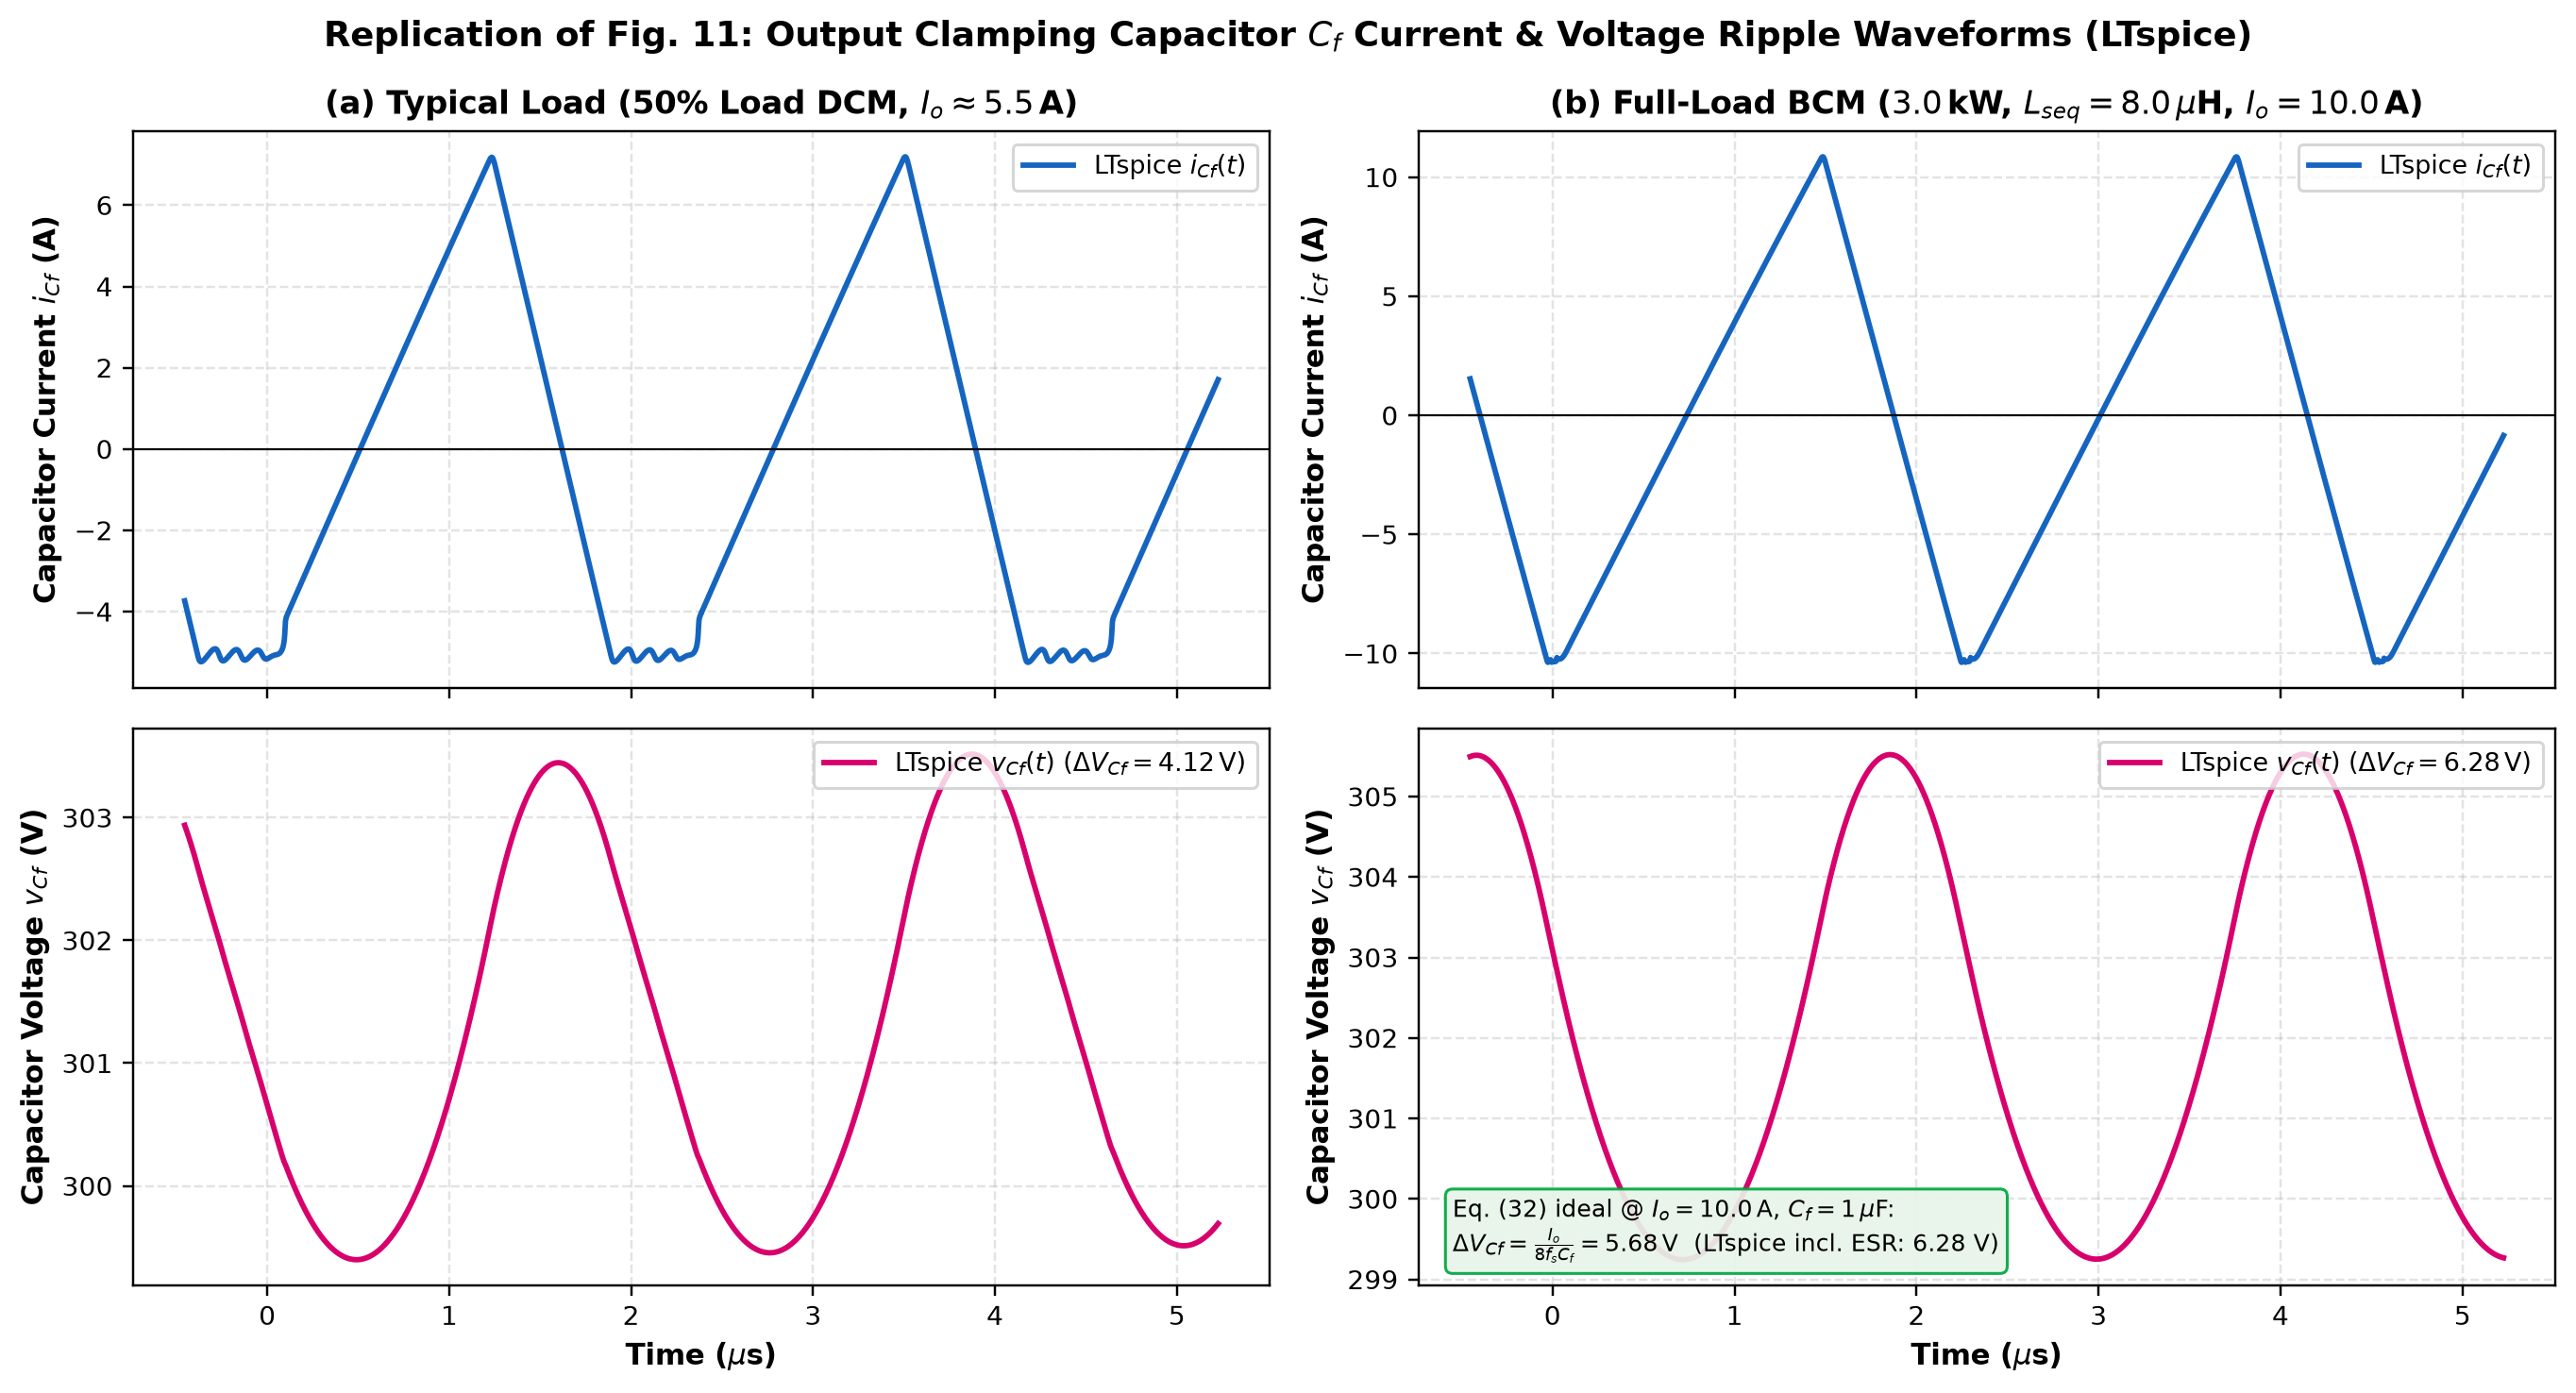
\includegraphics[width=\textwidth,height=6.2cm,keepaspectratio]{fig11_output_capacitor_waveforms.png}
    \end{column}
  \end{columns}
\end{frame}

% ==============================================================================
% SEZIONE 6: SIMULAZIONI LTSPICE SU TUTTO IL CARICO (0%-100%)
% ==============================================================================
\section{6. Simulazioni LTspice (0--100\%)}

% --- SLIDE 23 ---
\begin{frame}{Modellazione in LTspice e Sintesi delle 17 Simulazioni Standalone}{Modelli SPICE calibrati da datasheet reali e quadro numerico dallo 0\% al 100\%}
  \begin{columns}[T,onlytextwidth]
    \begin{column}{0.39\textwidth}
      \scriptsize
      \textbf{\color{PrimaryBlue}Fedelt\`a fisica della suite LTspice:}
      \begin{itemize}\setlength{\itemsep}{2pt}
        \item \textbf{17 file \texttt{.asc} + \texttt{.plt}} su griglia 16\,px, verificati da \texttt{asc\_compiler.py} (0 pin flottanti, 0 corti).
        \item \textbf{MOSFET \texttt{STW77N65M5}} (VDMOS): $V_{to}=4\V$, $R_d+R_s=34\mOhm$ (44\,m$\Omega$ a caldo per efficienza), capacit\`a non lineari $C_{gd}, C_{gs}, C_{jo}$.
        \item \textbf{Diodi SiC \texttt{CPW2\_0600S010B}}: $T_t = 0$, $B_v=600\V$, $C_{jo}=460\pF$, $R_s=55\mOhm$.
        \item \textbf{Diodi Si \texttt{D\_FRED\_1200V}} (PSFB conv.): $T_t = 55\ns$ (\emph{reverse recovery} reale!), $B_v=1200\V$.
        \item \textbf{Parassiti realistici:} $C_w=35\pF$ ($65\Ohm$), $C_s=140\pF$, $R_{bat}=0.15\Ohm$, perdite rame/nucleo ($R_{pri}, R_{aux}, R_{\text{core}}$) per Fig.\,23.
      \end{itemize}
      \vspace*{1mm}
      \begin{formulabox}
        \textbf{Controllo del punto di lavoro:} basta variare \texttt{.param psi=...} (da $13.5^\circ$ a vuoto fino a $151^\circ$ al 100\%).
      \end{formulabox}
    \end{column}
    \begin{column}{0.59\textwidth}
      \centering
      \scriptsize
      \setlength{\tabcolsep}{2.6pt}
      \renewcommand{\arraystretch}{1.18}
      \begin{tabular}{@{}lcccccc@{}}
        \toprule
        \textbf{Test (Fig.)} & $\boldsymbol{\psi}$ & $\boldsymbol{P_o}$ & $\boldsymbol{I_{s,\text{pk}}}$ & $\boldsymbol{I_{s,\text{rms}}}$ & $\boldsymbol{V_{D2,\min}}$ & \textbf{Reg.} \\
        \midrule
        0\% No-Load (15) & $13.5^\circ$ & $23.9\W$ & $1.70\A$ & $0.57\A$ & $-301.2\V$ & DCM \\
        10\% Load (16)   & $44.8^\circ$ & $324.3\W$ & $6.62\A$ & $2.44\A$ & $-302.4\V$ & DCM \\
        25\% Load (17)   & $71.0^\circ$ & $857.0\W$ & $10.88\A$ & $5.00\A$ & $-303.7\V$ & DCM \\
        50\% Load (18)   & $99.5^\circ$ & $1524.7\W$ & $14.50\A$ & $7.66\A$ & $-305.1\V$ & DCM \\
        70\% Load (19)   & $116.5^\circ$ & $2028.2\W$ & $16.68\A$ & $9.43\A$ & $-305.4\V$ & $\approx$BCM \\
        85\% Load (20)   & $123.5^\circ$ & $2616.7\W$ & $19.04\A$ & $11.50\A$ & $-305.9\V$ & \color{WarnAmber}\textbf{CCM} \\
        100\% Load (21)  & $151.0^\circ$ & $3002.8\W$ & $21.17\A$ & $13.16\A$ & $-306.8\V$ & \color{AlertRed}\textbf{CCM} \\
        \midrule
        BCM corr.\ $8\uH$ & $119.5^\circ$ & $3113.9\W$ & $25.08\A$ & $14.32\A$ & $-307.5\V$ & \color{GoodGreen}\textbf{BCM} \\
        Conv.\ 10\% (14a) & $114.0^\circ$ & $335.0\W$ & --- & --- & \color{AlertRed}\textbf{$-634.7\V$} & CCM \\
        Conv.\ 100\% (14b)& $124.5^\circ$ & $2904.1\W$ & --- & --- & \color{AlertRed}\textbf{$-959.2\V$} & CCM \\
        \bottomrule
      \end{tabular}

      \vspace*{1.5mm}
      {\tiny\color{MutedGray}Misure estratte via direttive \texttt{.meas} di LTspice (\texttt{results/simulation\_metrics.json}). Clamping di $V_{D2,\min}$ tra $-301\V$ e $-307\V$ sull'intera dinamica 0--3\,kW!}
    \end{column}
  \end{columns}
\end{frame}

% --- SLIDE 24 ---
\begin{frame}{Confronto Diretto Stress sui Diodi: Proposto vs.\ Convenzionale (Bonus 2)}{Riduzione del 68\% della tensione inversa di picco a pieno carico ($3\kW$, $V_o=300\V$)}
  \centering
  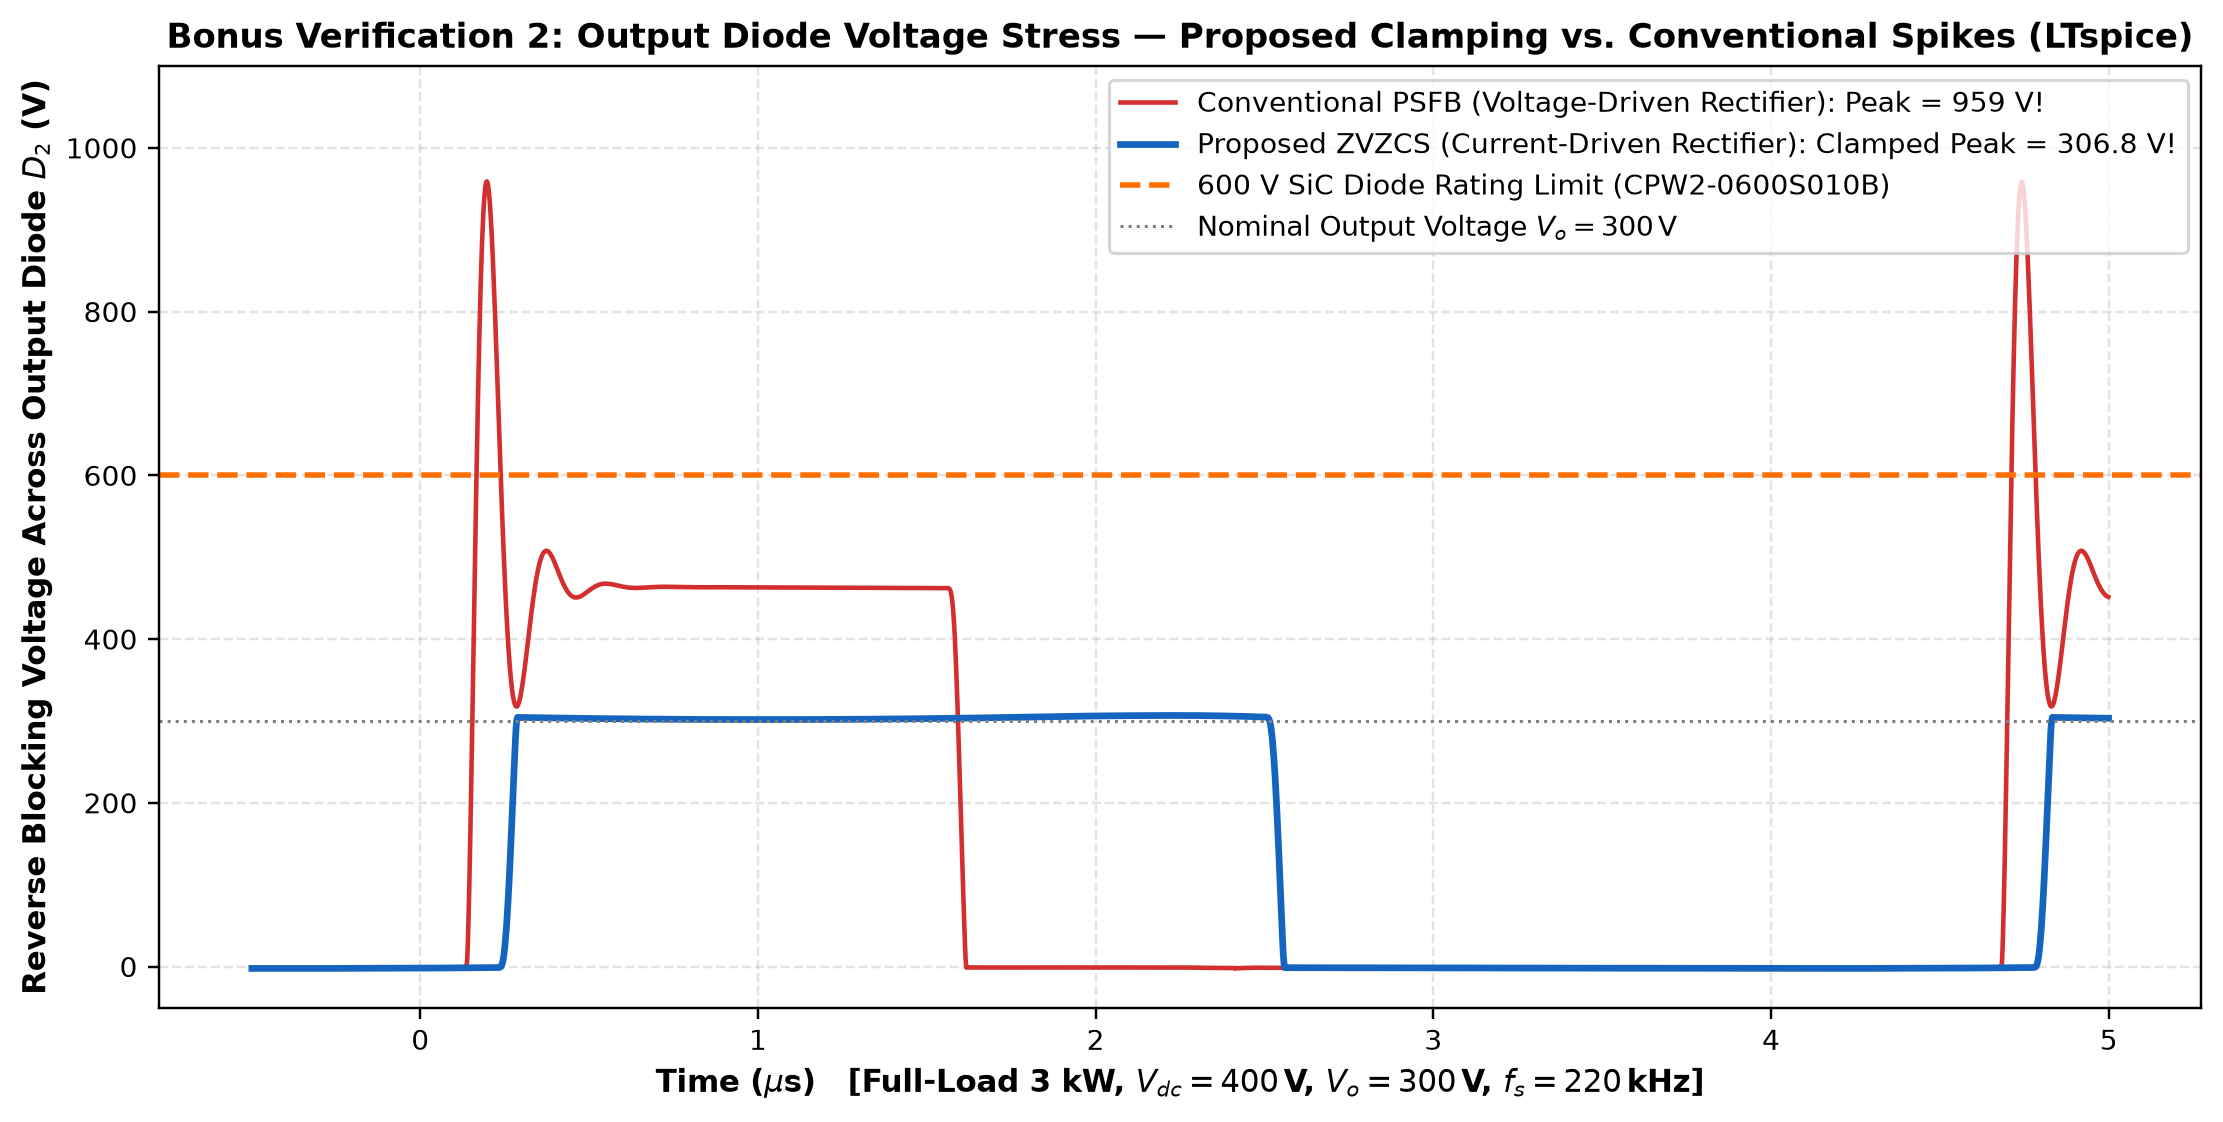
\includegraphics[width=0.80\textwidth,height=4.35cm,keepaspectratio]{bonus02_proposed_vs_conventional_diode_spikes.png}

  \vspace*{1.5mm}
  \begin{columns}[T,onlytextwidth]
    \begin{column}{0.49\textwidth}
      \begin{warnbox}[title={PSFB Convenzionale (curva rossa) --- Voltage-Driven}]
        \begin{itemize}\setlength{\itemsep}{1pt}
          \item Tensione inversa di picco su $D_2$: \textbf{959\,V} ($3.2\times V_o$!), sfonda ampiamente il limite di $600\V$ (linea arancione tratteggiata).
          \item Impone diodi Si da \textbf{1200\,V} + snubber R-C dissipativo + grosso filtro EMI.
        \end{itemize}
      \end{warnbox}
    \end{column}
    \begin{column}{0.49\textwidth}
      \begin{okbox}[title={Topologia Proposta (curva blu) --- Current-Driven}]
        \begin{itemize}\setlength{\itemsep}{1pt}
          \item Tensione inversa di picco rigorosamente clampata a \textbf{306.8\,V} ($V_o + \Delta V_{Cf}/2$, \textbf{$-68\%$ di stress}!).
          \item Abilita diodi \textbf{SiC Schottky da 600\,V} con ampio margine ($\approx 2\times$), zero $Q_{rr}$ e nessun circuito snubber!
        \end{itemize}
      \end{okbox}
    \end{column}
  \end{columns}
\end{frame}

% --- SLIDE 25 ---
\begin{frame}{Funzionamento a Carico Nullo: 0\% No-Load (Fig.\,15)}{Verifica di funzionamento affidabile, zero spike e ZVS completo a fine carica batteria}
  \centering
  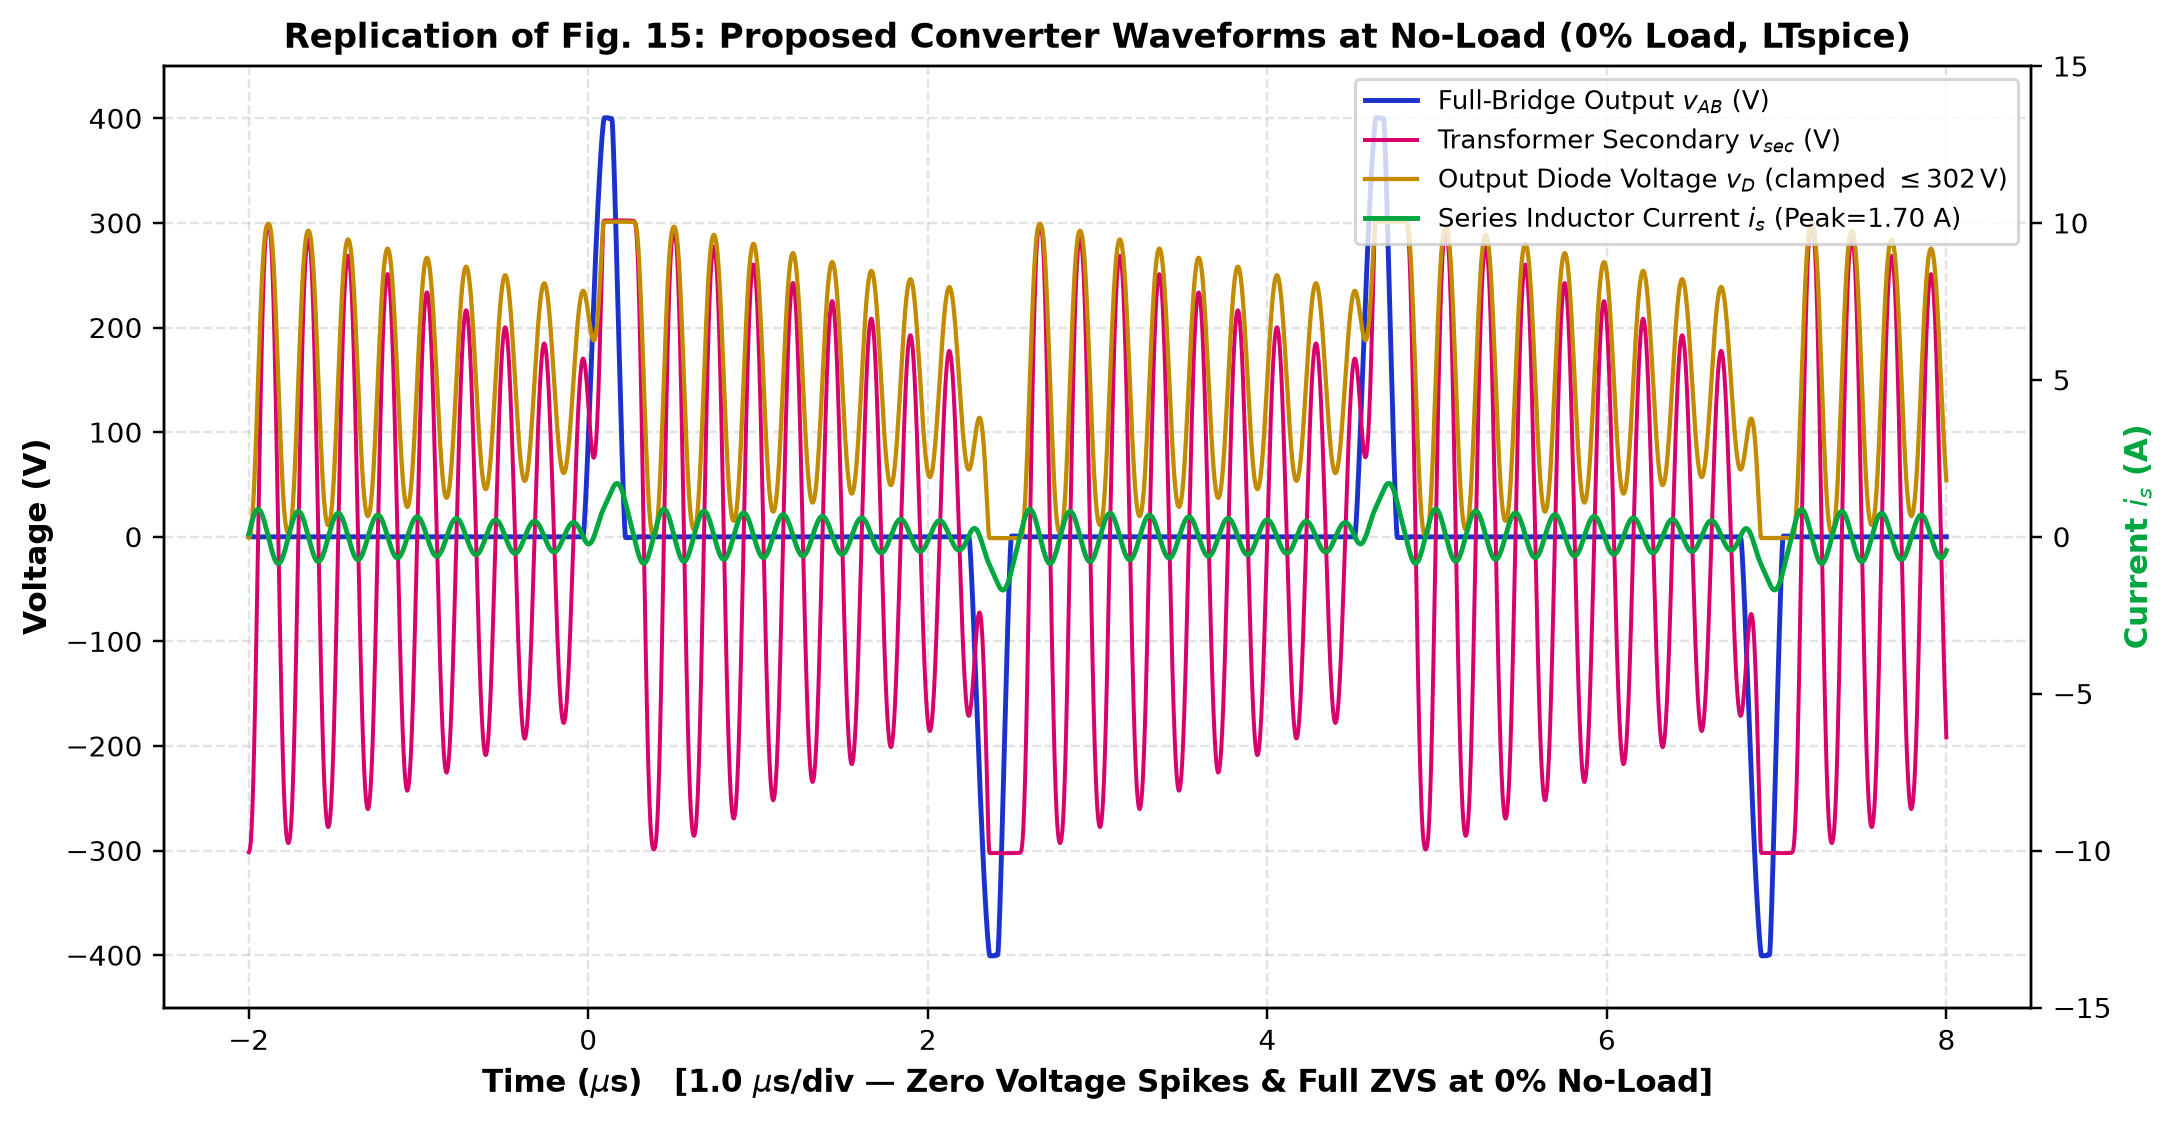
\includegraphics[width=0.82\textwidth,height=4.25cm,keepaspectratio]{fig15_proposed_noload.png}

  \vspace*{1.5mm}
  \begin{columns}[T,onlytextwidth]
    \begin{column}{0.49\textwidth}
      \scriptsize
      \textbf{\color{PrimaryBlue}Lettura del grafico (\texttt{05\_proposed\_noload\_fig15.asc}, $\psi=13.5^\circ$):}
      \begin{itemize}\setlength{\itemsep}{1.5pt}
        \item \textbf{$v_{AB}$ (blu)}: impulsi strettissimi a $\pm 400\V$ ($t_{on}\approx 5\ns$ effettivi); potenza quasi nulla ($23.9\W$, pari allo $0.8\%$ di $3\kW$).
        \item \textbf{$i_s$ (verde)}: piccolo impulso ($I_{s,\text{pk}}=1.70\A$), seguito da debole corrente oscillatoria di risonanza.
        \item \textbf{$v_D$ (oro) e $v_{sec}$ (magenta)}: tensione sul diodo rigorosamente $\le \mathbf{301.2\V}$ (zero sovratensioni!).
      \end{itemize}
    \end{column}
    \begin{column}{0.49\textwidth}
      \begin{okbox}[title={Fenomeni fisici chiave a No-Load}]
        \begin{itemize}\setlength{\itemsep}{1.2pt}
          \item \textbf{Lungo Modo VII}: quasi l'intero semiperiodo \`e occupato dall'oscillazione parassita smorzata a $\mathbf{4.7\MHz}$ tra $L_{seq}/k^2$ e $C_w+C_j$ (oscilla tra $0\V$ e $+300\V$, mai sopra $V_o$!).
          \item \textbf{ZVS 100\% mantenuto}: nonostante $i_s\approx 0$, i due induttori ausiliari $L_{AUX1}=L_{AUX2}=67\uH$ forniscono i $\pm 3.39\A$ necessari a scaricare $2C_{so}$ su entrambe le gambe!
        \end{itemize}
      \end{okbox}
    \end{column}
  \end{columns}
\end{frame}

% --- SLIDE 26 ---
\begin{frame}{Funzionamento a Carico Leggero: 10\% / 300\,W (Fig.\,16)}{DCM profondo, clamping pulito e confronto diretto con il PSFB convenzionale (Fig.\,14a)}
  \centering
  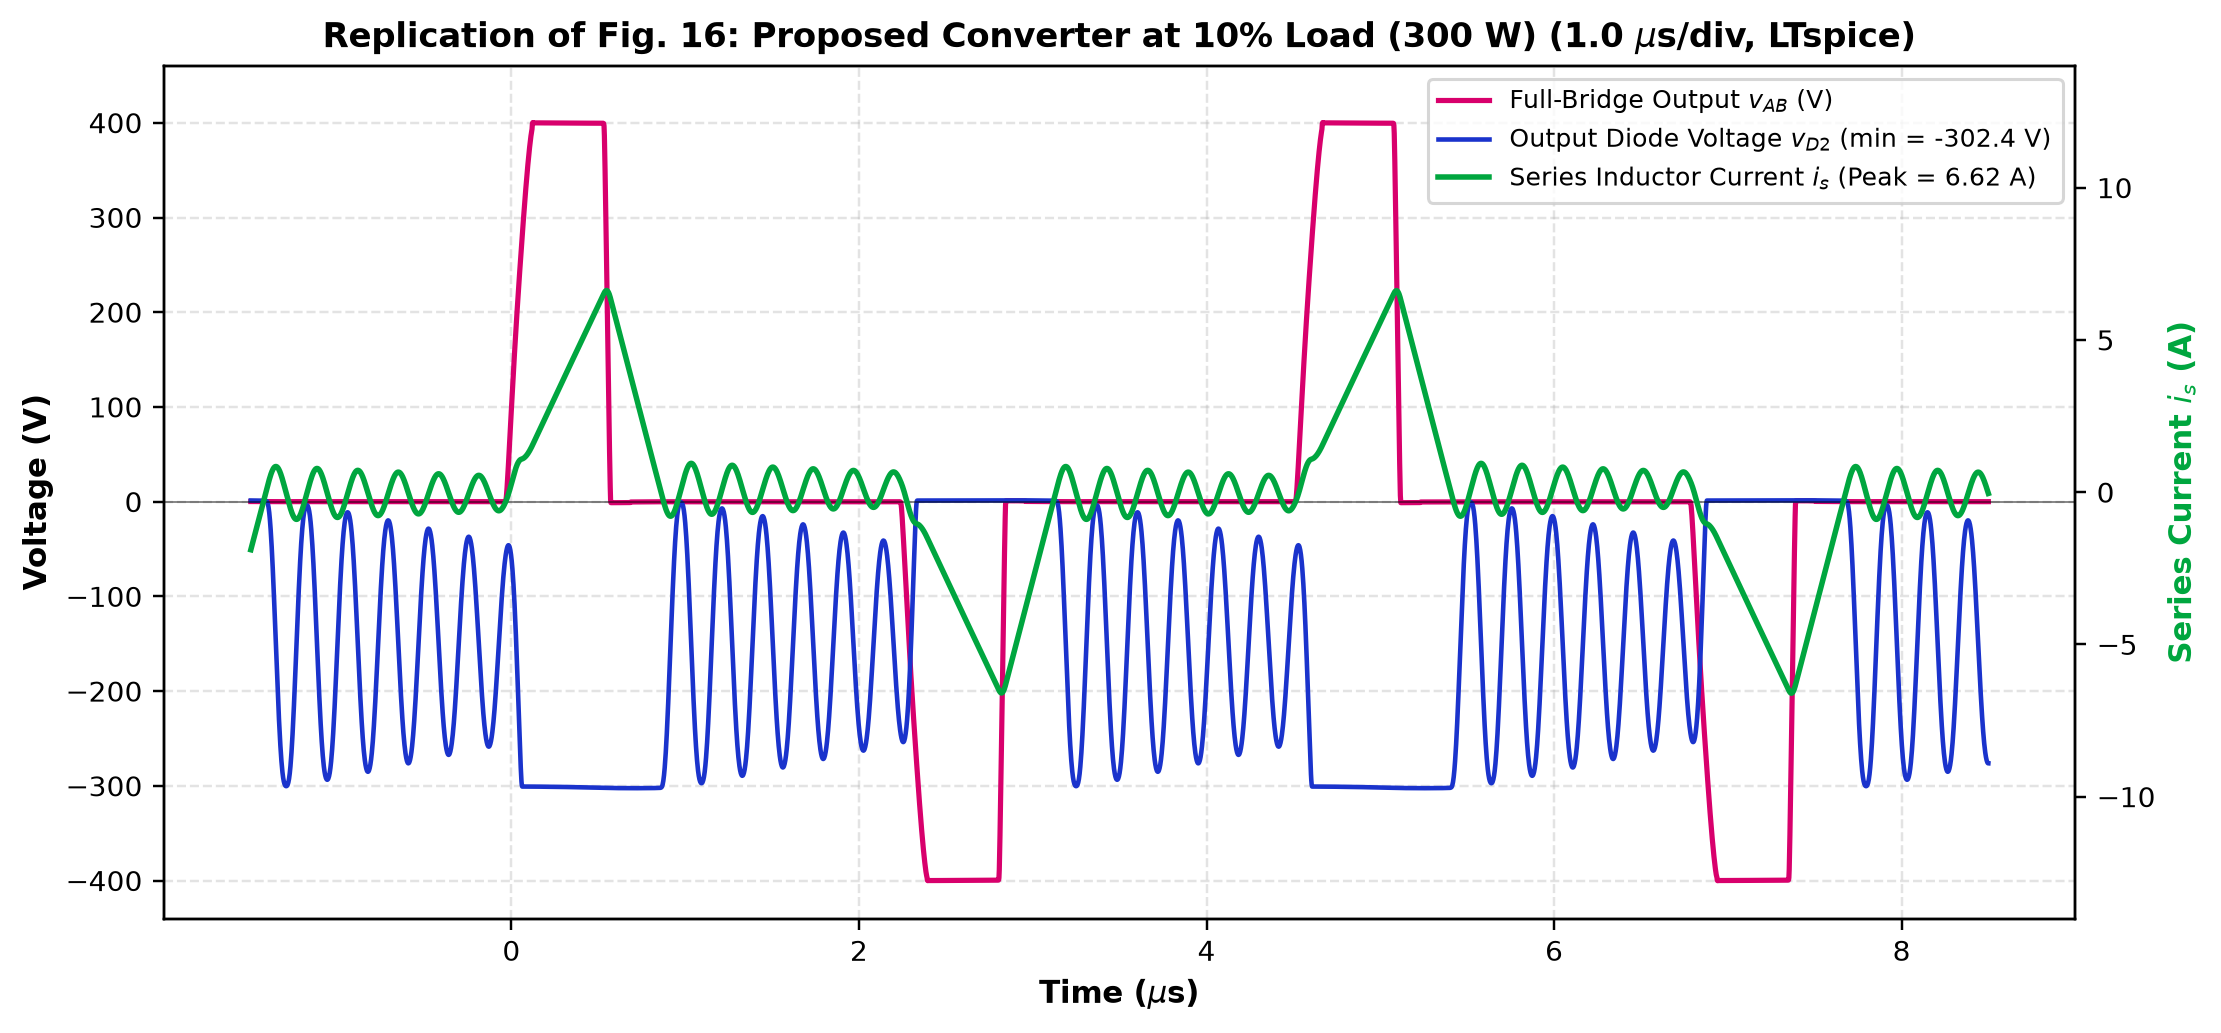
\includegraphics[width=0.84\textwidth,height=4.20cm,keepaspectratio]{fig16_proposed_10pct.png}

  \vspace*{1.5mm}
  \begin{columns}[T,onlytextwidth]
    \begin{column}{0.49\textwidth}
      \scriptsize
      \textbf{\color{PrimaryBlue}Misure LTspice (\texttt{06\_proposed\_load\_10pct\_fig16.asc}, $\psi=44.8^\circ$):}
      \begin{itemize}\setlength{\itemsep}{1.5pt}
        \item $P_o = \mathbf{324.3\W}$ ($I_o = 1.08\A$), $I_{s,\text{pk}} = \mathbf{6.62\A}$, $I_{s,\text{rms}} = 2.44\A$, efficienza stadio $\eta = 97.50\%$.
        \item \textbf{$v_{AB}$ (magenta)}: impulso netto $\pm 400\V$ di durata $t_{on}\approx 0.40\us$, seguito da smagnetizzazione $t_{off}\approx 0.23\us$ e lungo Modo VII ($\approx 1.6\us$).
        \item \textbf{$v_{D2}$ (blu)}: $0\V$ in conduzione, clampata piatta a \textbf{$-302.4\V$} in blocco, poi ringing smorzato attorno a $-V_o/2=-150\V$ in Modo VII.
      \end{itemize}
    \end{column}
    \begin{column}{0.49\textwidth}
      \begin{okbox}[title={Confronto diretto: Fig.\,16 (Proposto) vs.\ Fig.\,14(a) (Conv.)}]
        \begin{itemize}\setlength{\itemsep}{1.2pt}
          \item A parit\`a di carico (10\%, $\sim 300\W$), il PSFB convenzionale genera gi\`a spike da \textbf{636\,V} sui diodi e ha efficienza $\eta = 92.24\%$.
          \item Qui la tensione inversa non supera mai \textbf{302.4\,V} (zero spike!) e lo spegnimento dei diodi al termine di ogni triangolo verde avviene a corrente esattamente nulla (\textbf{ZCS naturale}).
        \end{itemize}
      \end{okbox}
    \end{column}
  \end{columns}
\end{frame}

% --- SLIDE 27 ---
\begin{frame}{Funzionamento al 25\% di Carico: 750\,W --- Vista Intera e Zoom (Fig.\,17a/b)}{Fronti ZVS morbidi, conferma visiva dello ZVZCS leading-leg e clamping su $v_{D2}$}
  \begin{columns}[T,onlytextwidth]
    \begin{column}{0.58\textwidth}
      \centering
      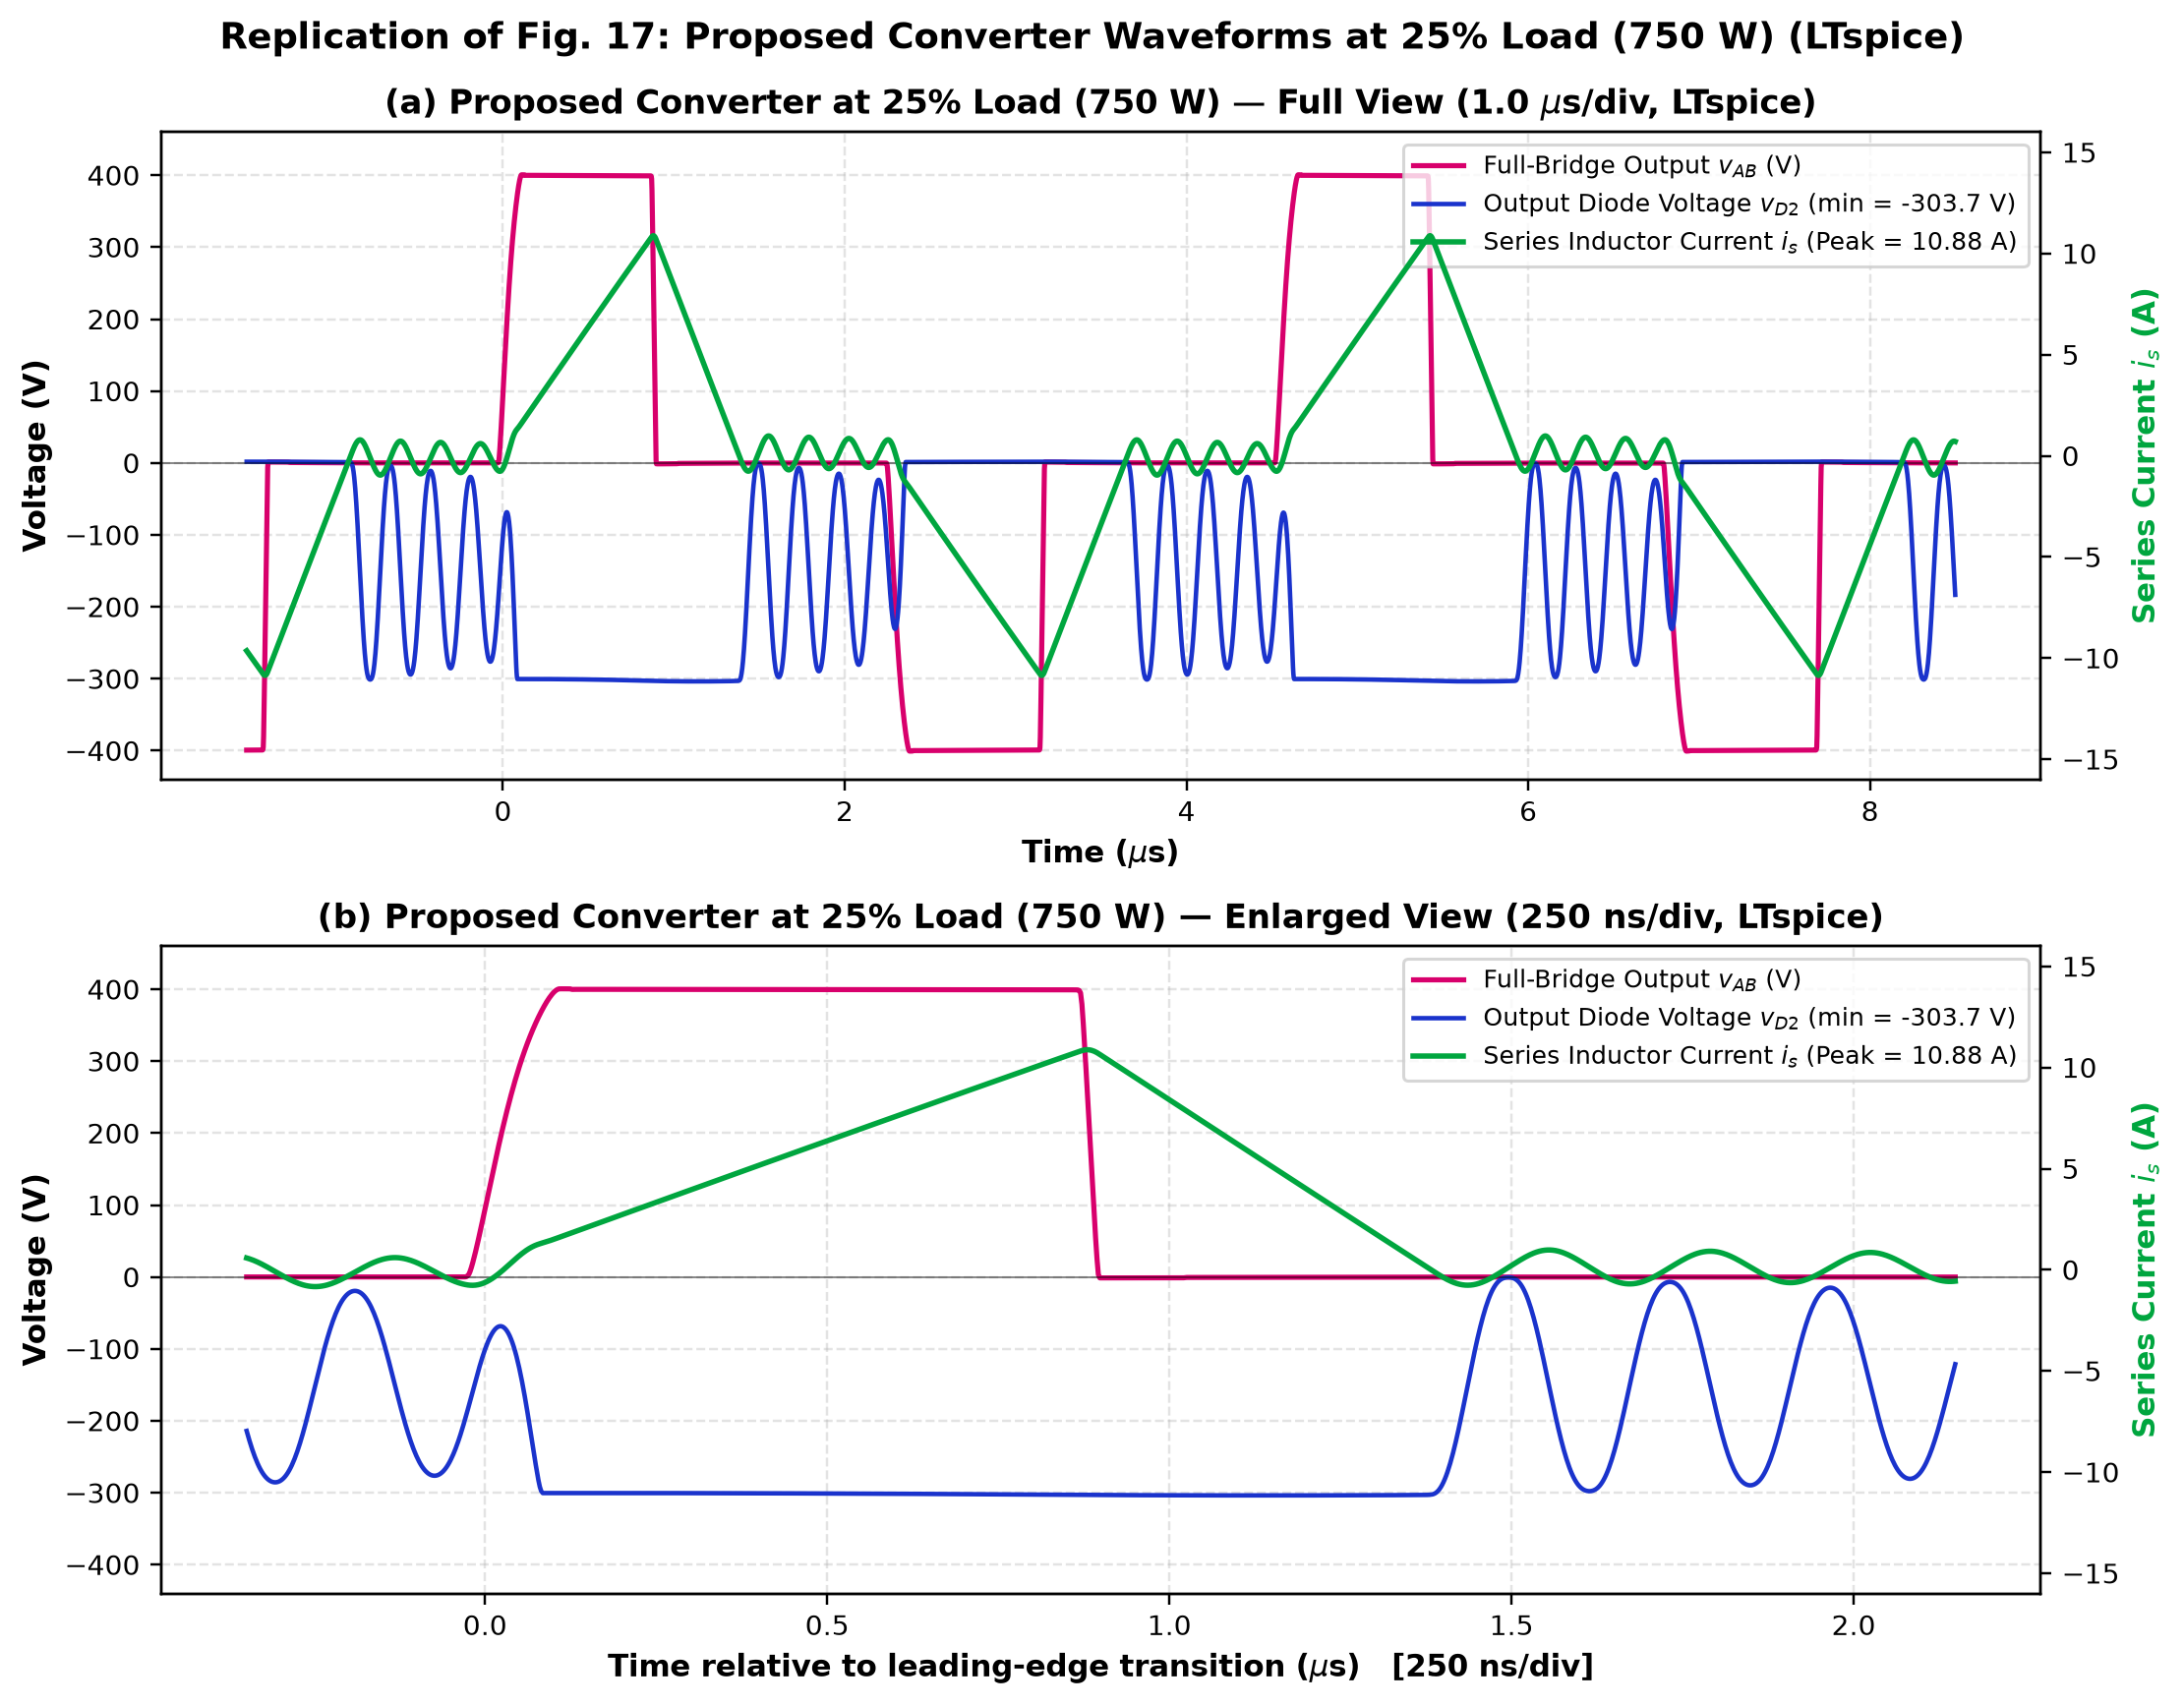
\includegraphics[width=\textwidth,height=6.25cm,keepaspectratio]{fig17_proposed_25pct_full_and_zoom.png}
    \end{column}
    \begin{column}{0.40\textwidth}
      \scriptsize
      \textbf{\color{PrimaryBlue}Misure LTspice (\texttt{07\_proposed\_load\_25pct}):}
      \begin{itemize}\setlength{\itemsep}{2.2pt}
        \item Sfasamento $\psi = \mathbf{71.0^\circ}$, $P_o = \mathbf{857.0\W}$ ($I_o = 2.85\A$), $I_{s,\text{pk}} = \mathbf{10.88\A}$, $I_{s,\text{rms}} = 5.00\A$, $\eta_{\text{nom}} = 98.04\%$.
        \item \textbf{Pannello (a) --- 1.0\,$\mu$s/div}: il triangolo di corrente $i_s$ si allarga ($t_{on}\approx 0.73\us$, $t_{off}\approx 0.42\us$) riducendo la durata del Modo VII (meno cicli di ringing blu rispetto al 10\%).
        \item \textbf{Pannello (b) --- Zoom 250\,ns/div}: si osservano chiaramente:
          \begin{enumerate}\setlength{\itemsep}{1.5pt}
            \item La rampa morbida ZVS di $v_{AB}$ (fronte \emph{leading} in $\sim 120\ns$, fronte \emph{lagging} ancora pi\`u rapido grazie a $I_p+I_{PB}$).
            \item $i_s \approx 0$ durante la salita di $v_{AB}$ $\Rightarrow$ prova visiva di \textbf{ZVZCS sulla gamba leading}!
            \item Il plateau piatto di $v_{D2}$ a \textbf{$-303.7\V$} senza alcun overshoot.
          \end{enumerate}
      \end{itemize}
    \end{column}
  \end{columns}
\end{frame}

% --- SLIDE 28 ---
\begin{frame}{Funzionamento al 50\% di Carico: 1500\,W --- Vista Intera e Zoom (Fig.\,18a/b)}{Punto di lavoro nominale DCM con assenza totale di spike e di freewheeling}
  \begin{columns}[T,onlytextwidth]
    \begin{column}{0.58\textwidth}
      \centering
      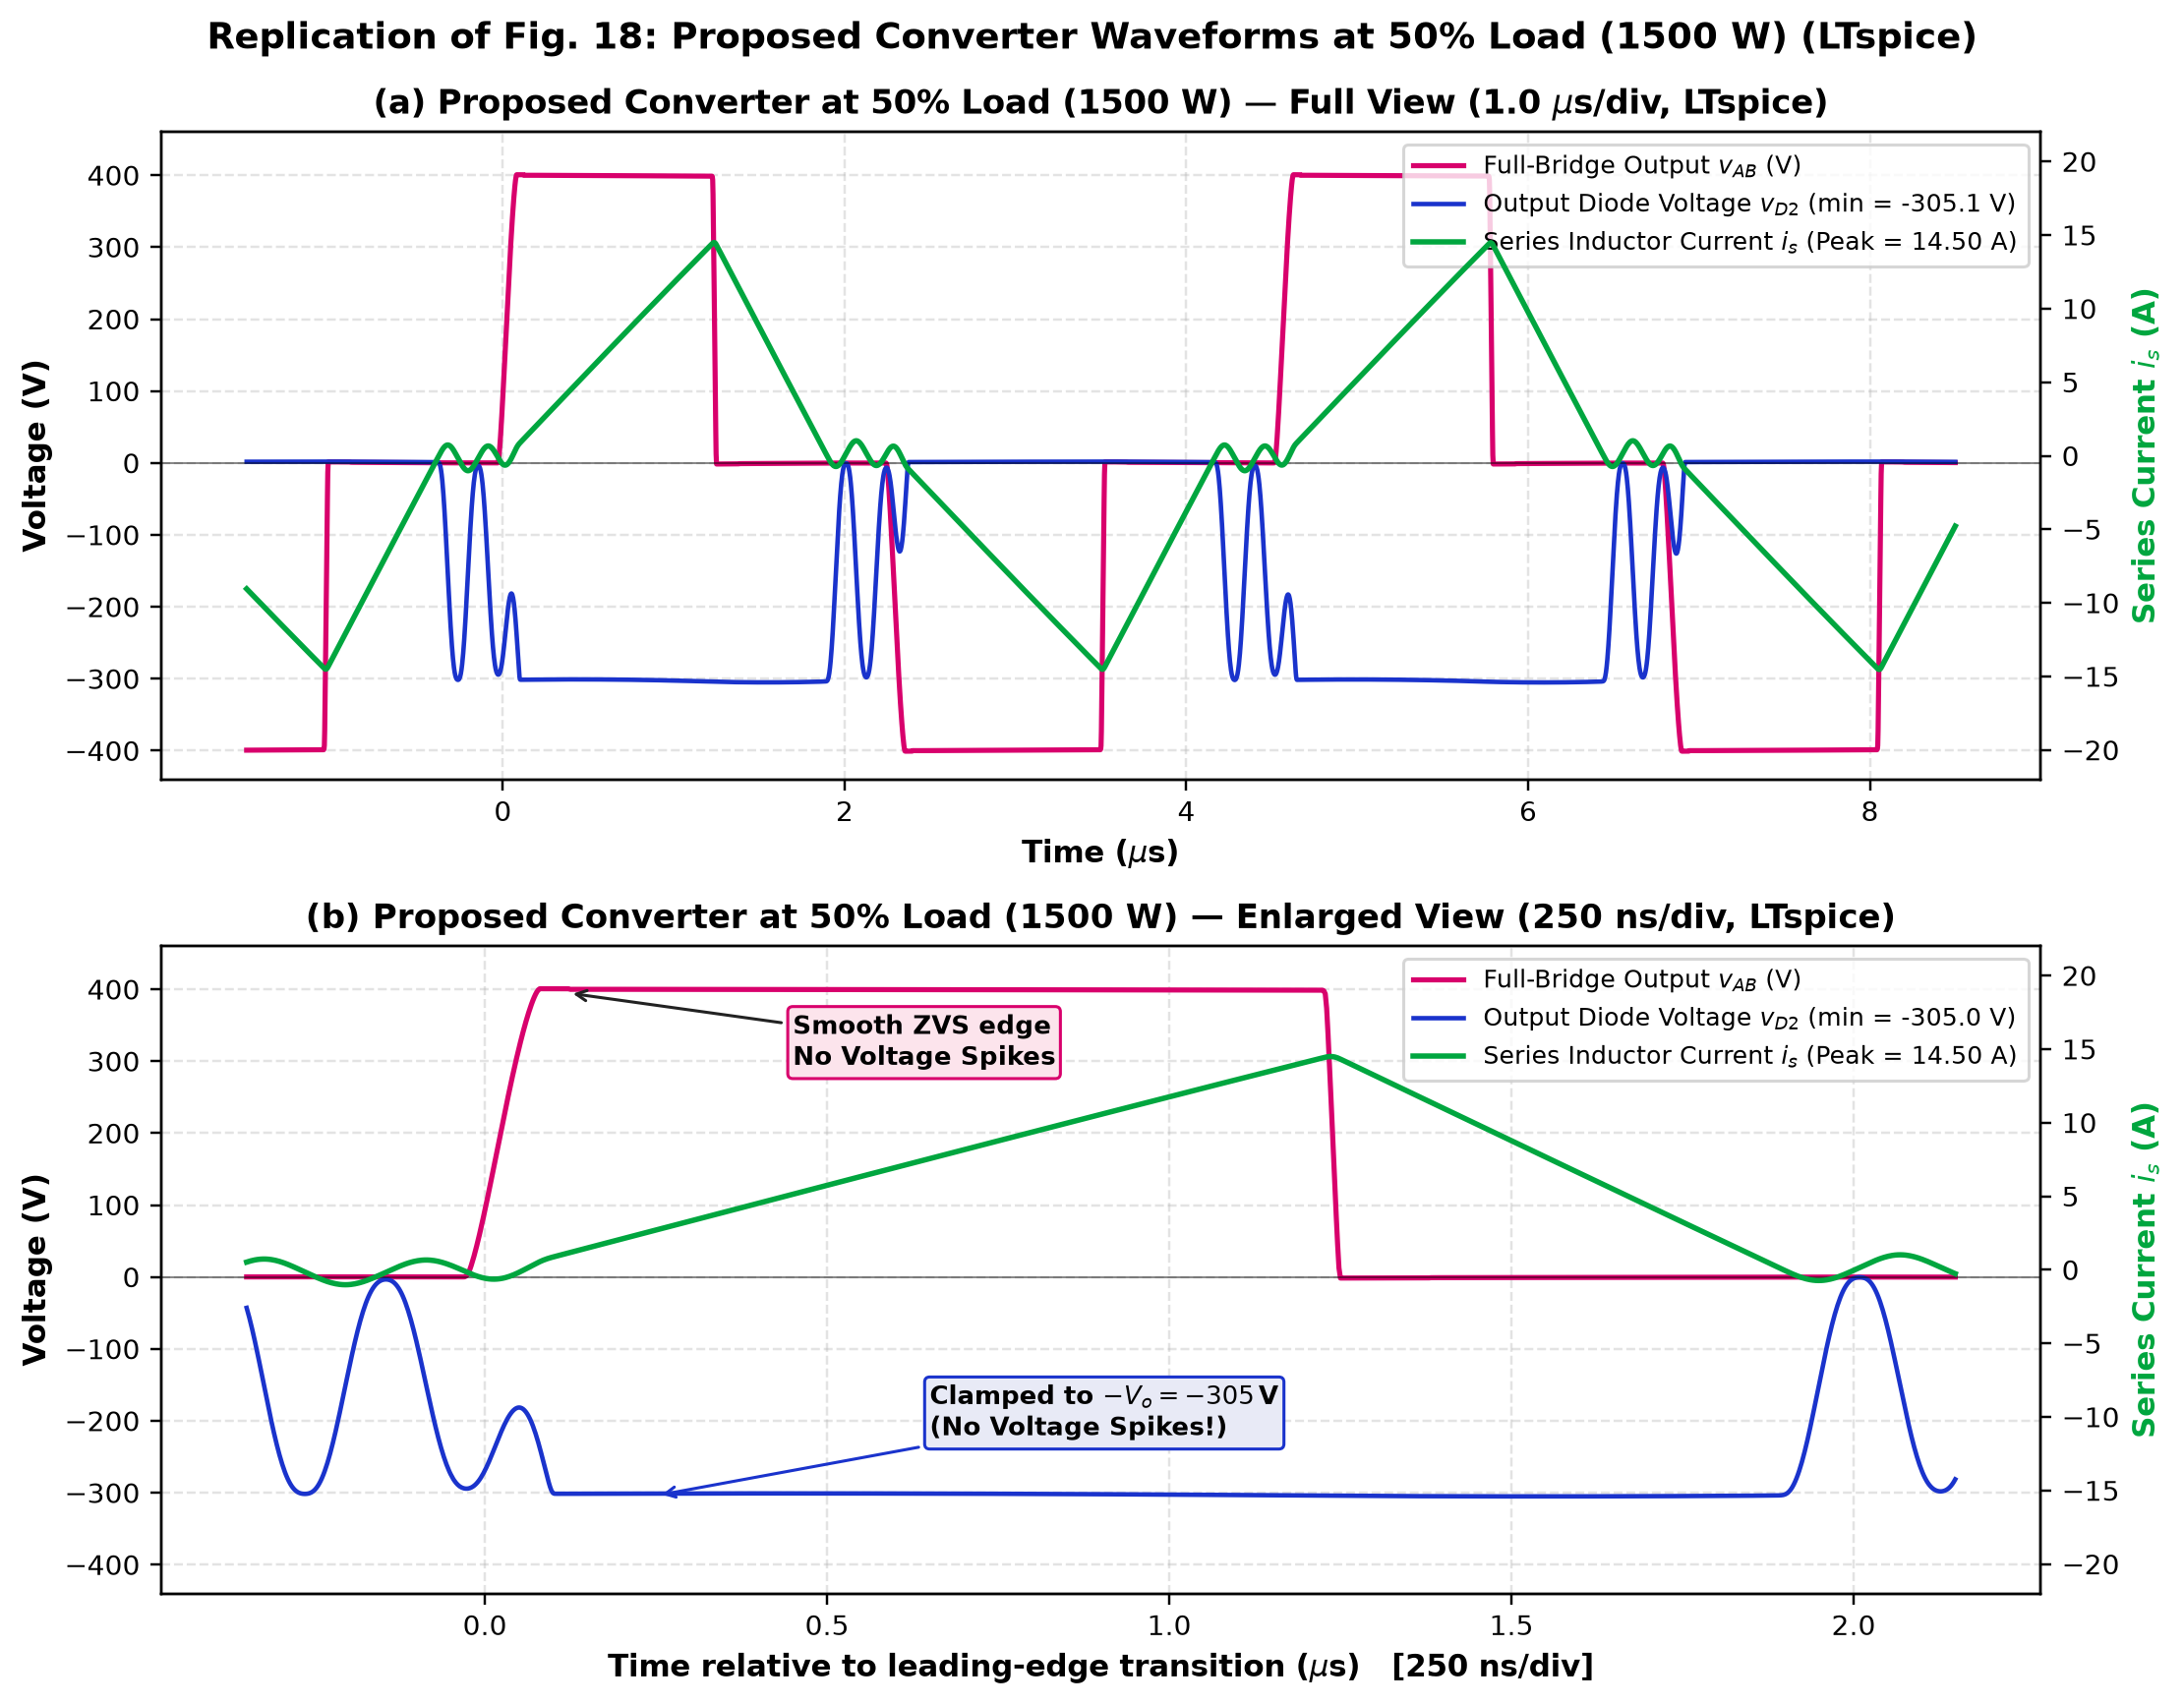
\includegraphics[width=\textwidth,height=6.25cm,keepaspectratio]{fig18_proposed_50pct_full_and_zoom.png}
    \end{column}
    \begin{column}{0.40\textwidth}
      \scriptsize
      \textbf{\color{PrimaryBlue}Misure LTspice (\texttt{08\_proposed\_load\_50pct}):}
      \begin{itemize}\setlength{\itemsep}{2pt}
        \item Sfasamento $\psi = \mathbf{99.5^\circ}$, $P_o = \mathbf{1524.7\W}$ ($I_o = 5.07\A$), $I_{s,\text{pk}} = \mathbf{14.50\A}$, $I_{s,\text{rms}} = 7.66\A$, $V_{D2,\min} = \mathbf{-305.1\V}$, $\eta_{\text{nom}} = 97.65\%$.
        \item \textbf{Pannello (a)}: funzionamento ancora in \textbf{DCM}; restano $\approx 0.35\us$ di Modo VII ($\sim 1.5$ cicli di oscillazione a $4.7\MHz$ su $v_{D2}$).
        \item \textbf{Pannello (b) --- Zoom 250\,ns/div}: replica fedelmente le annotazioni ``\emph{No Voltage Spikes}'' di Fig.\,18(b) sia sul fronte ZVS di $v_{AB}$ sia sui fronti di $v_{D2}$.
        \item \textbf{Verifica $t_{off}/t_{on}$}: sullo zoom si misura $t_{on}\approx 1.15\us$ e $t_{off}\approx 0.65\us \Rightarrow t_{off}/t_{on}=\mathbf{0.56}$ (identico al calcolo teorico per $300\V/400\V$!).
      \end{itemize}
      \vspace*{1mm}
      \begin{okbox}
        Notare inoltre $\psi=99.5^\circ$ (esattamente come nell'oscillogramma Fig.\,18 del paper), smentendo i $\approx 45^\circ$ di Fig.\,7!
      \end{okbox}
    \end{column}
  \end{columns}
\end{frame}

% --- SLIDE 29 ---
\begin{frame}{Funzionamento al 70\% di Carico: 2100\,W --- Avvicinamento al BCM (Fig.\,19a/b)}{Il Modo VII si riduce quasi a zero: il prototipo con $L_{seq}=11.8\uH$ \`e gi\`a al limite critico!}
  \begin{columns}[T,onlytextwidth]
    \begin{column}{0.58\textwidth}
      \centering
      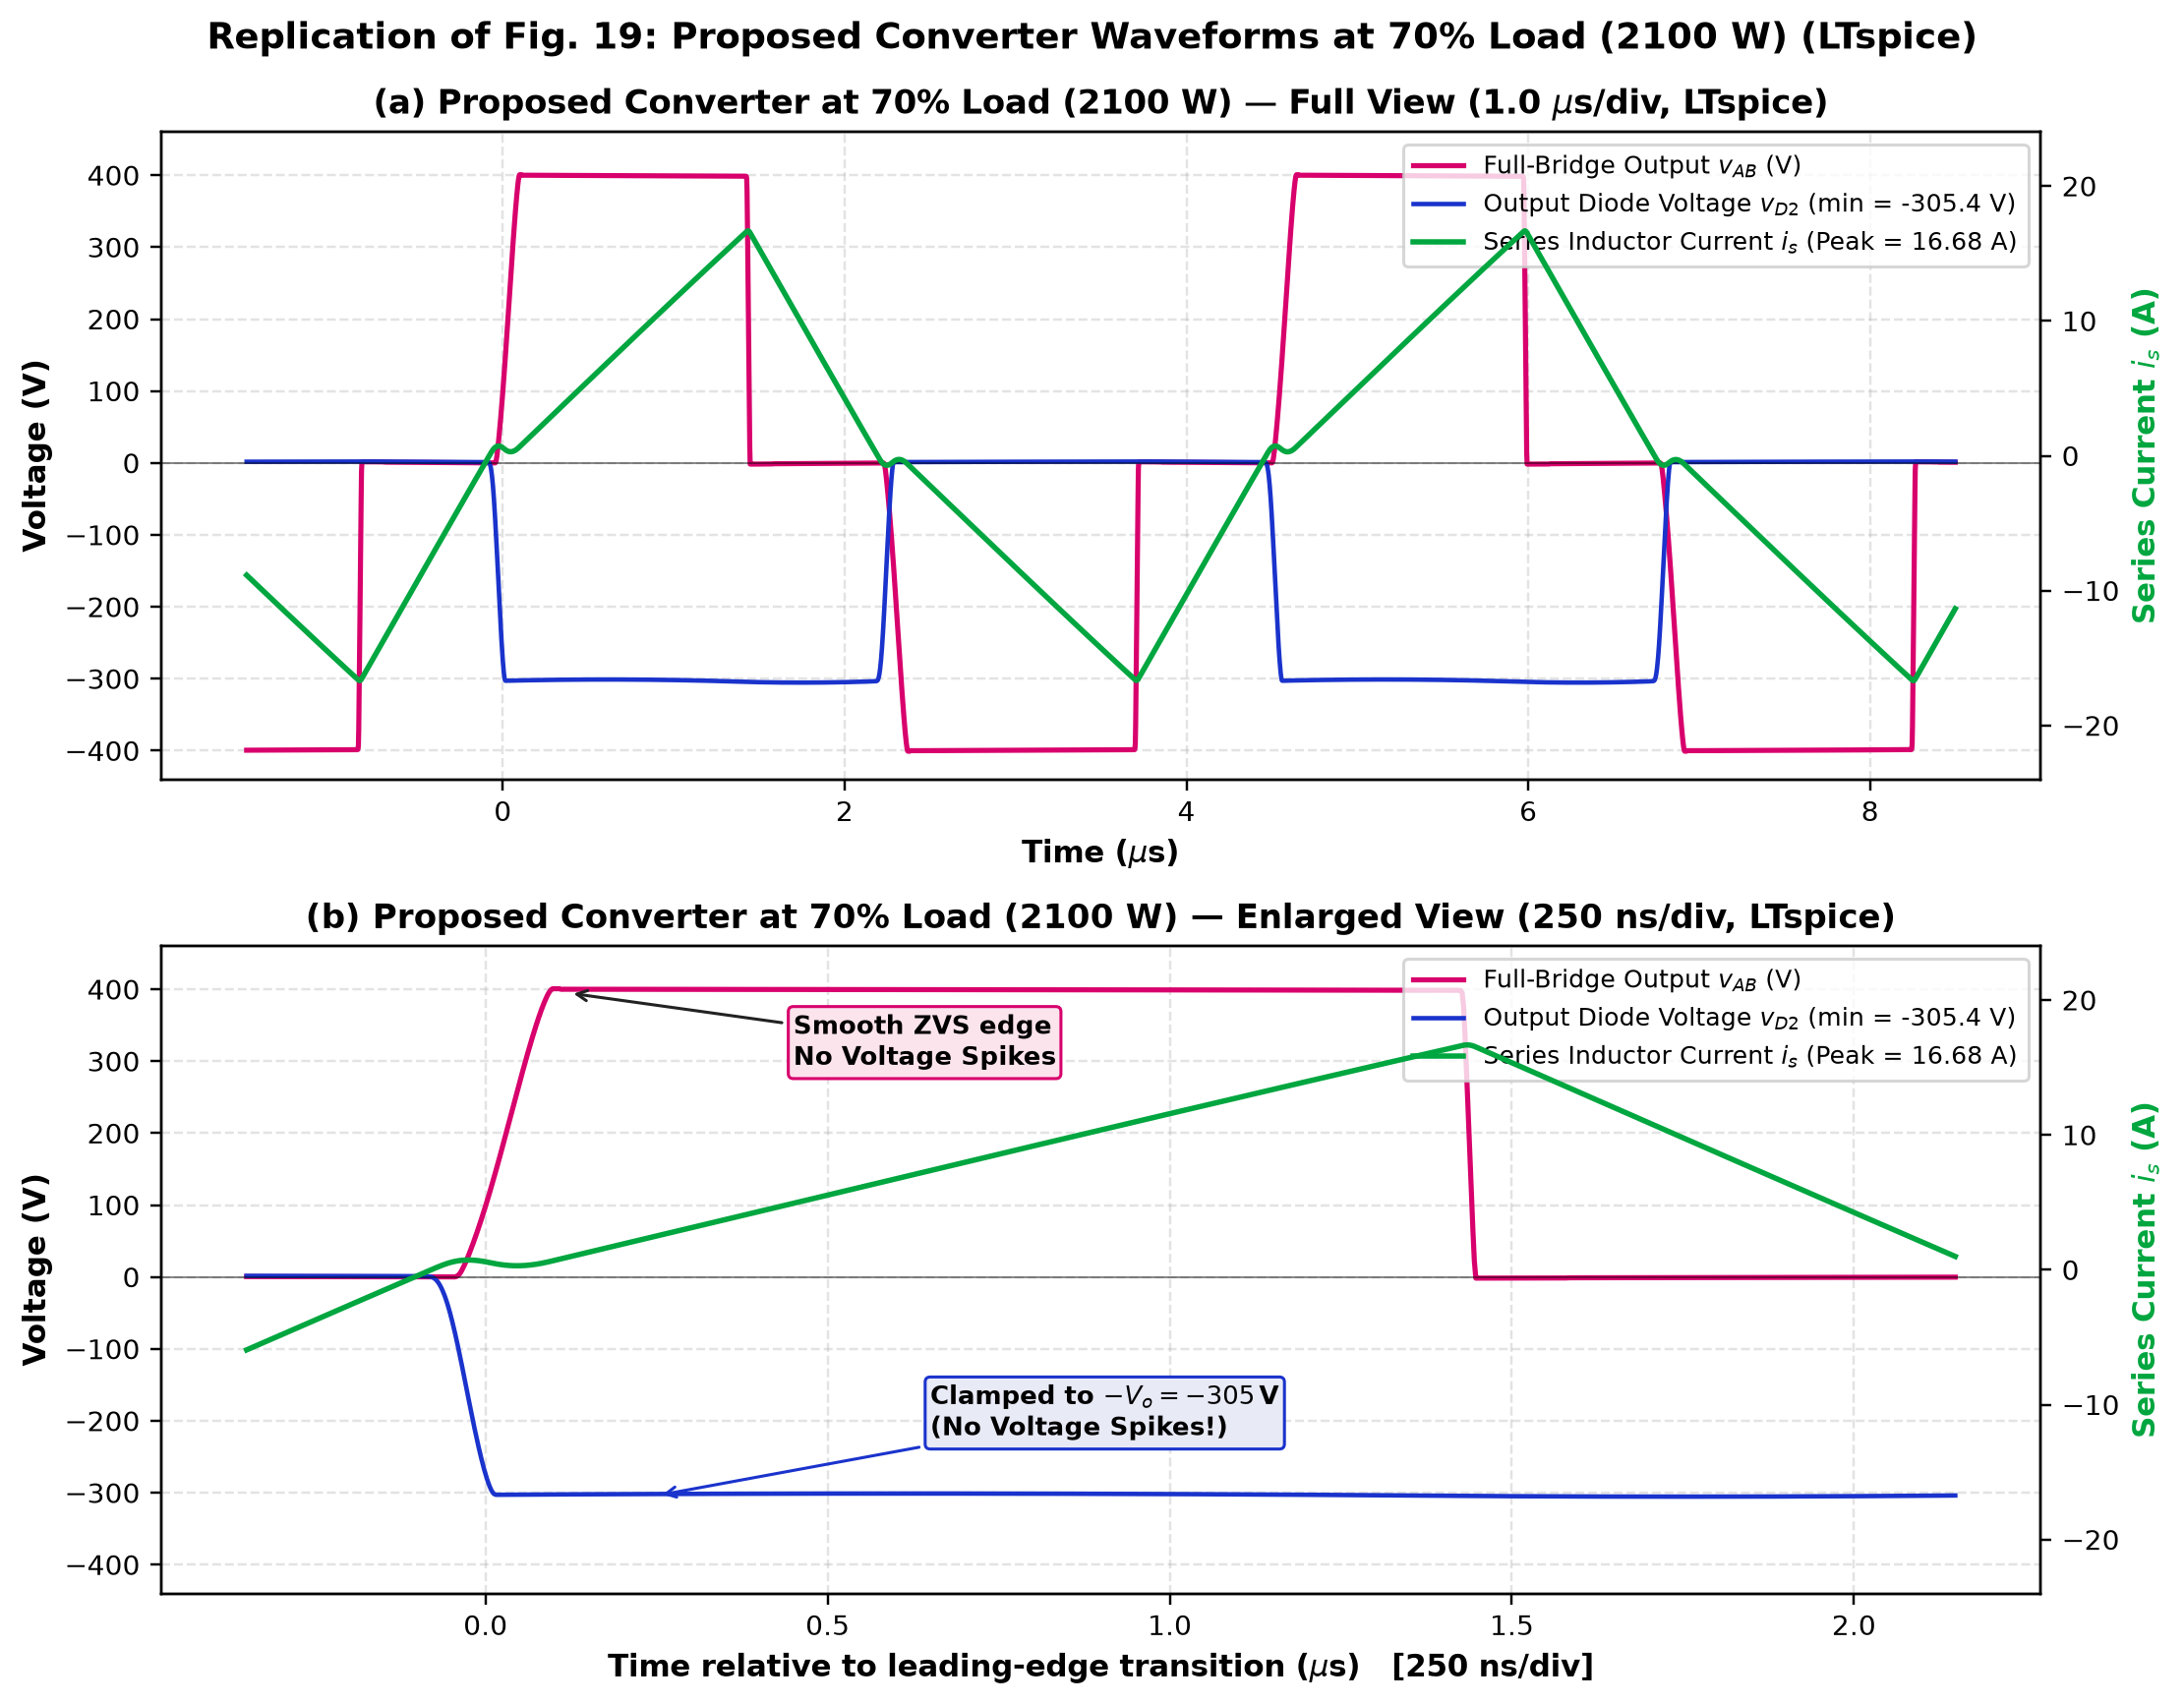
\includegraphics[width=\textwidth,height=6.25cm,keepaspectratio]{fig19_proposed_70pct_full_and_zoom.png}
    \end{column}
    \begin{column}{0.40\textwidth}
      \scriptsize
      \textbf{\color{PrimaryBlue}Misure LTspice (\texttt{09\_proposed\_load\_70pct}):}
      \begin{itemize}\setlength{\itemsep}{2pt}
        \item Sfasamento $\psi = \mathbf{116.5^\circ}$, $P_o = \mathbf{2028.2\W}$ ($I_o = 6.74\A$), $I_{s,\text{pk}} = \mathbf{16.68\A}$, $I_{s,\text{rms}} = 9.43\A$, $V_{D2,\min} = \mathbf{-305.4\V}$, $\eta_{\text{nom}} = 97.95\%$.
        \item \textbf{Evoluzione fisica rispetto al 50\%}: come osservato anche dal paper, al crescere del carico i \textbf{Modi IV--VI} (rampa di discesa di $i_s$) guadagnano rilevanza fino a saturare l'intero semiperiodo!
        \item \textbf{Scomparsa del Modo VII}: in pannello (a) $i_s$ tocca zero praticamente nell'istante $t_7 = 2.27\us$ in cui inizia il semiperiodo negativo $\Rightarrow$ \textbf{il ringing a $4.7\MHz$ sparisce completamente}!
      \end{itemize}
      \vspace*{1mm}
      \begin{notebox}[title={Punto Critico di Soglia BCM}]
        Con $L_{seq}=11.8\uH$ (Tab.\,II), la soglia teorica BCM \`e \textbf{$2.27\kW$ (75.6\% di carico)}: al 70\% siamo l'ultimo punto operativo in cui valgono ancora ZVZCS \emph{leading} e ZCS naturale dei diodi!
      \end{notebox}
    \end{column}
  \end{columns}
\end{frame}

% --- SLIDE 30 ---
\begin{frame}{Funzionamento all'85\% di Carico: 2550\,W --- Ingresso in CCM! (Fig.\,20a/b)}{Superata la soglia BCM di $2.27\kW$, $i_s$ non si annulla pi\`u prima della transizione leading}
  \begin{columns}[T,onlytextwidth]
    \begin{column}{0.58\textwidth}
      \centering
      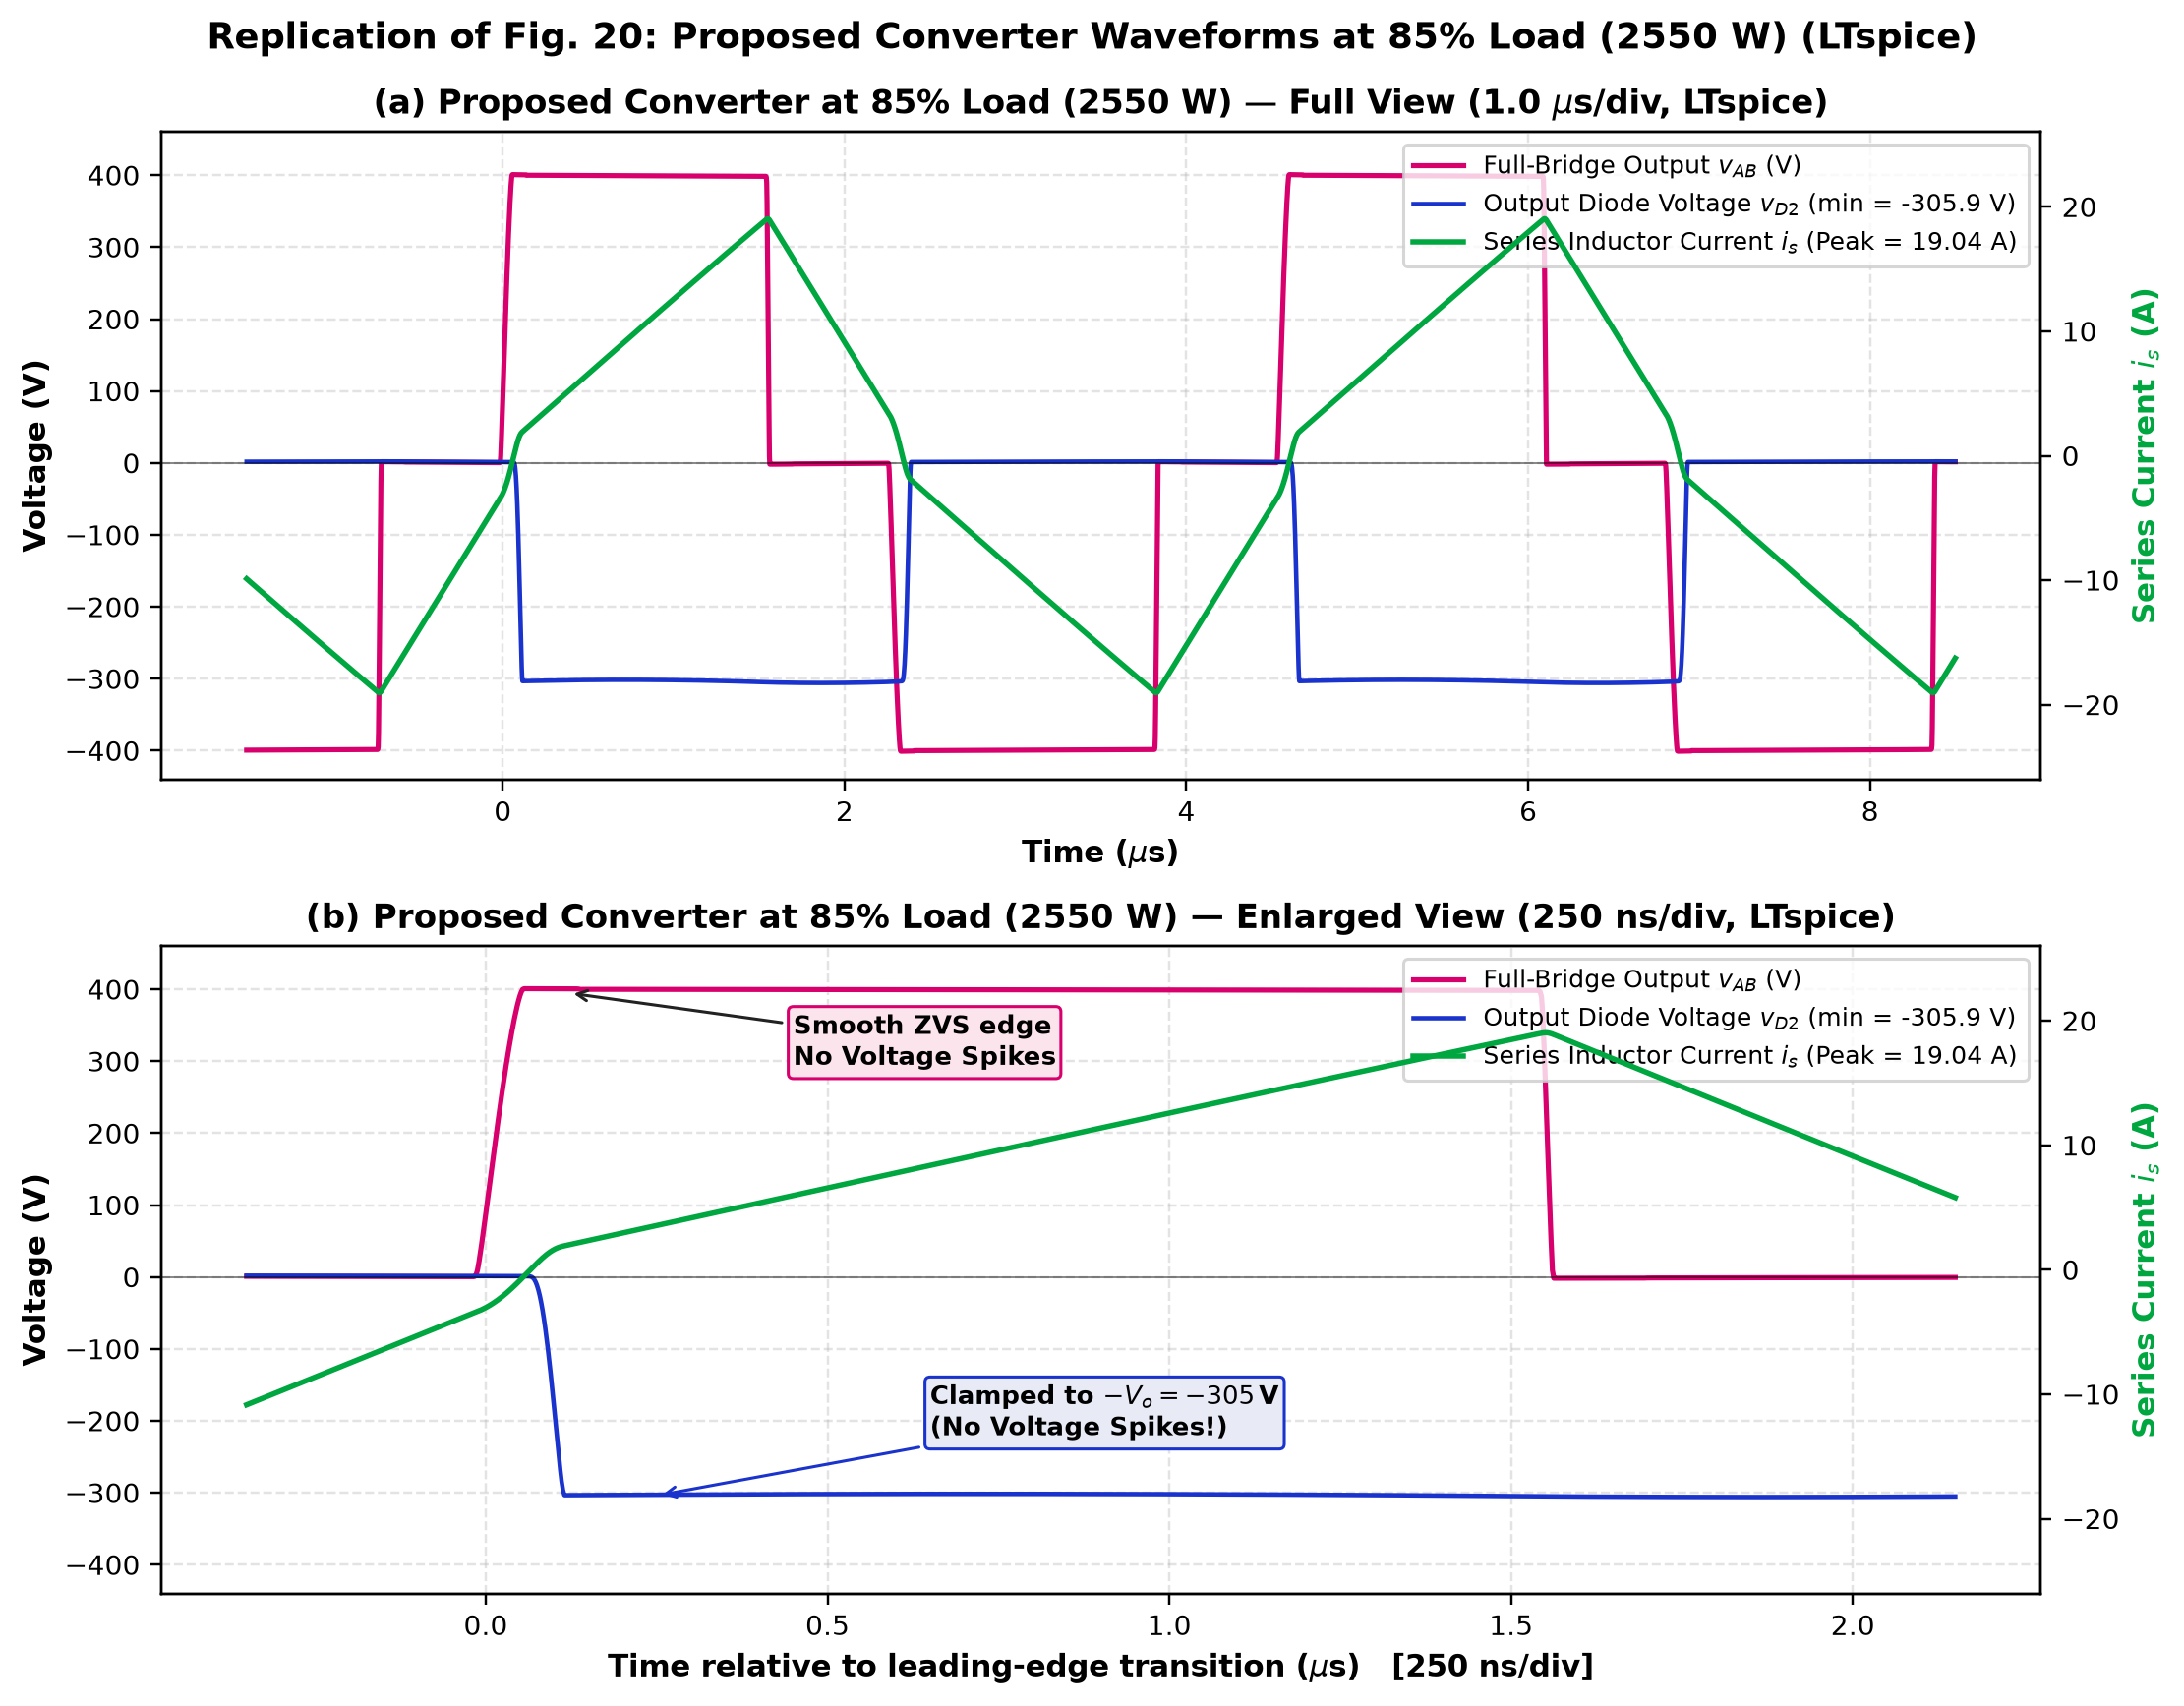
\includegraphics[width=\textwidth,height=6.25cm,keepaspectratio]{fig20_proposed_85pct_full_and_zoom.png}
    \end{column}
    \begin{column}{0.40\textwidth}
      \scriptsize
      \textbf{\color{PrimaryBlue}Misure LTspice (\texttt{10\_proposed\_load\_85pct}):}
      \begin{itemize}\setlength{\itemsep}{2pt}
        \item Sfasamento $\psi = \mathbf{123.5^\circ}$, $P_o = \mathbf{2616.7\W}$ ($I_o = 8.68\A$), $I_{s,\text{pk}} = \mathbf{19.04\A}$, $I_{s,\text{rms}} = 11.50\A$, $V_{D2,\min} = \mathbf{-305.9\V}$, $\eta_{\text{nom}} = 97.77\%$.
        \item \textbf{Prova visiva dell'ingresso in CCM}:
          \begin{itemize}\setlength{\itemsep}{1.2pt}
            \item Sullo zoom (b), a $t=0\us$ (fronte di salita di $v_{AB}$), $i_s$ \textbf{non \`e zero} ma parte ancora negativa ($\approx -3\A$) e cambia pendenza bruscamente!
            \item Il Modo VII \`e scomparso al 100\%: nessuna oscillazione parassita su $v_{D2}$.
          \end{itemize}
        \item \textbf{Clamping ancora intatto}: grazie a $C_f$ prima di $L_f$ e ai diodi SiC ($Q_{rr}=0$), anche in CCM $v_{D2}$ resta rigidamente clampata a \textbf{$-305.9\V$} senza sovratensioni!
      \end{itemize}
      \vspace*{1mm}
      \begin{warnbox}
        Dall'85\% in su la gamba \emph{leading} conserva lo ZVS ma \textbf{perde progressivamente lo ZCS} all'accensione.
      \end{warnbox}
    \end{column}
  \end{columns}
\end{frame}

% --- SLIDE 31 ---
\begin{frame}{Pieno Carico 100\% (3\,kW --- Fig.\,21): Scoperta CCM vs.\ Vero BCM}{Dimostrazione LTspice che il prototipo ($11.8\uH$) \`e in CCM profondo, e ripristino del BCM con $8.0\uH$}
  \begin{columns}[T,onlytextwidth]
    \begin{column}{0.58\textwidth}
      \centering
      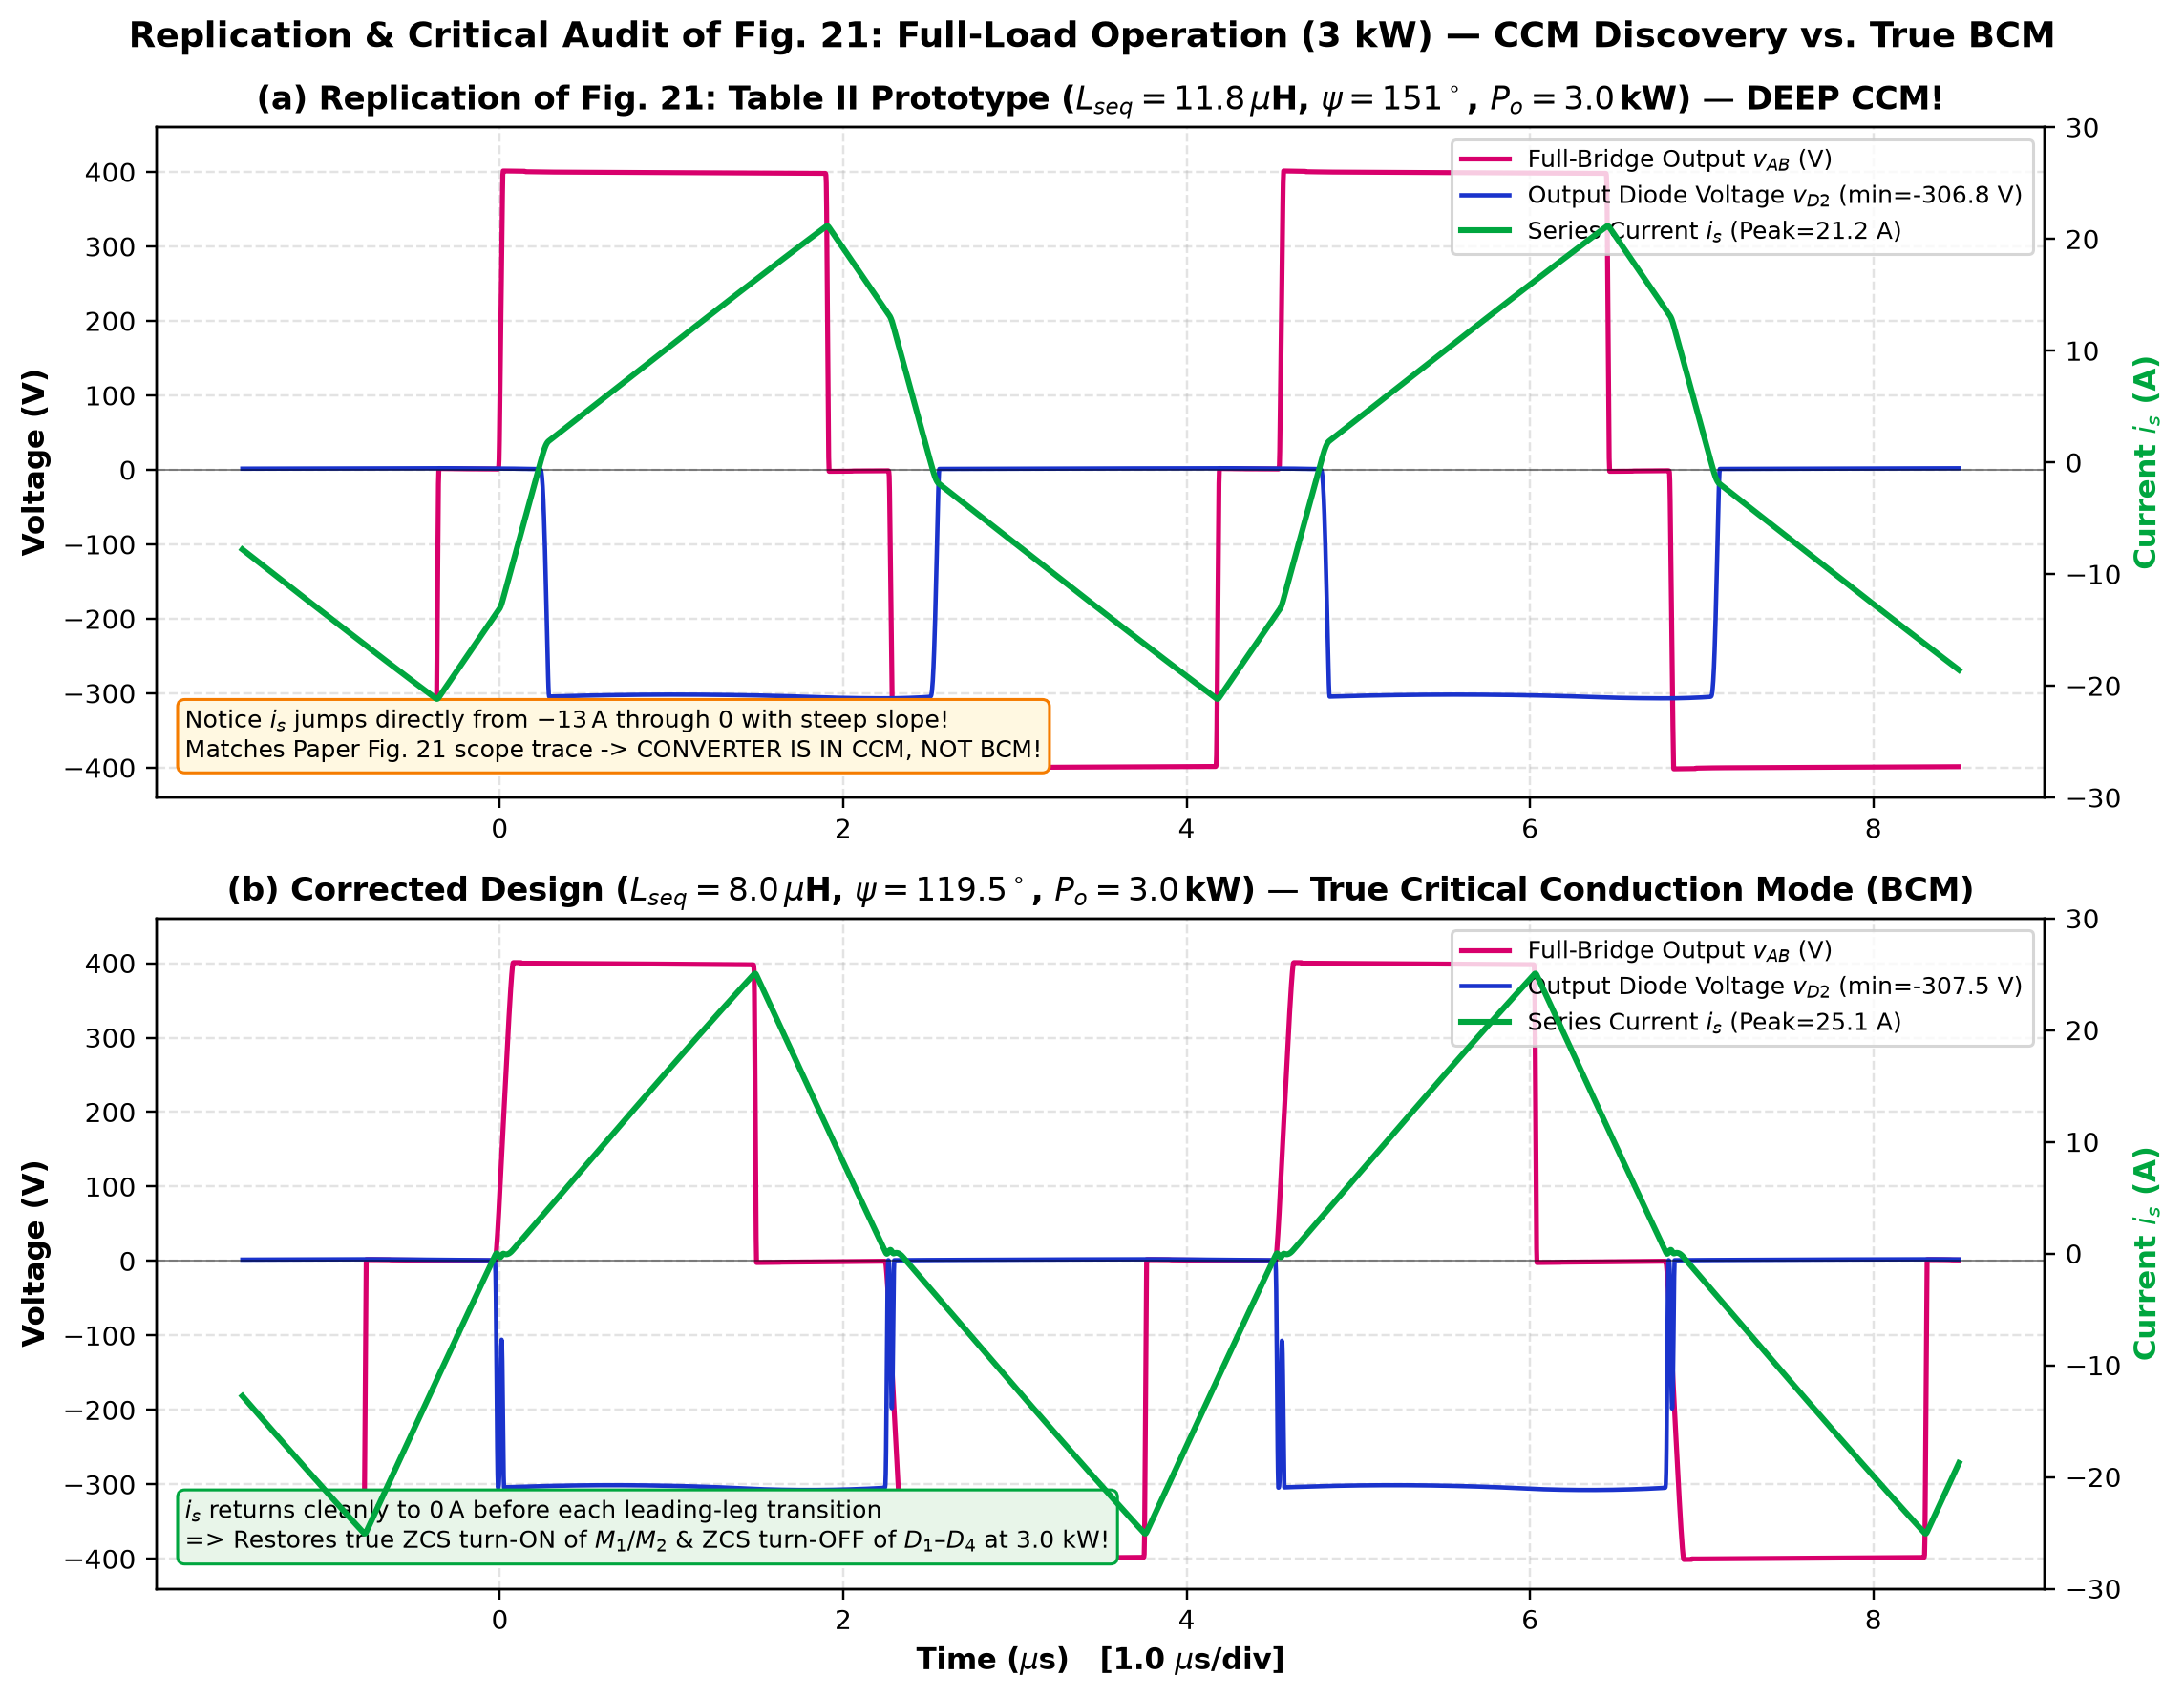
\includegraphics[width=\textwidth,height=6.25cm,keepaspectratio]{fig21_proposed_100pct_ccm_vs_bcm.png}
    \end{column}
    \begin{column}{0.40\textwidth}
      \scriptsize
      \textbf{\color{PrimaryBlue}Pannello (a) --- Prototipo Tab.\,II ($L_{seq}=11.8\uH$, $\psi=151^\circ$):}
      \begin{itemize}\setlength{\itemsep}{1.8pt}
        \item $P_o = \mathbf{3002.8\W}$, $I_{s,\text{pk}} = 21.17\A$, $I_{s,\text{rms}} = \mathbf{13.16\A}$ (coerente col rating $12.6\A_{\text{rms}}$ di Tab.\,II!), $V_{D2,\min} = -306.8\V$.
        \item \textbf{CCM profondo evidente:} $i_s$ taglia lo zero da $-13\A$ con pendenza ripidissima $\frac{V_{dc}+kV_o}{L_{seq}} \approx \mathbf{55.7\A/\us}$! Identico all'oscillogramma Fig.\,21 del paper (che a p.\,2766 dichiara erroneamente ``\emph{close to BCM}'').
        \item \textbf{Conseguenza:} perdita di ZCS sia sui MOSFET \emph{leading} sia sui diodi d'uscita (commutazione forzata a $55\A/\us$, sostenibile solo grazie ai diodi SiC!).
      \end{itemize}
      \vspace*{1.5mm}
      \begin{okbox}[title={Pannello (b) --- Progetto Corretto ($L_{seq}=8.0\uH$, $\psi=119.5^\circ$)}]
        Eroga $3.0\text{--}3.1\kW$ ($I_o\approx 10\A, I_{s,\text{pk}}=25.1\A$) in \textbf{vero Critical Conduction Mode}: $i_s$ torna pulita a $0\A$ prima di ogni transizione \emph{leading}, ripristinando pienamente ZVZCS e ZCS a pieno carico!
      \end{okbox}
    \end{column}
  \end{columns}
\end{frame}

% --- SLIDE 32 ---
\begin{frame}{Corrente del Circuito Ausiliario al Variare del Carico (Fig.\,22a/b)}{Dimostrazione dell'invarianza di $i_{LAUX1}$ dal 12\% fino al 100\% di carico}
  \begin{columns}[T,onlytextwidth]
    \begin{column}{0.58\textwidth}
      \centering
      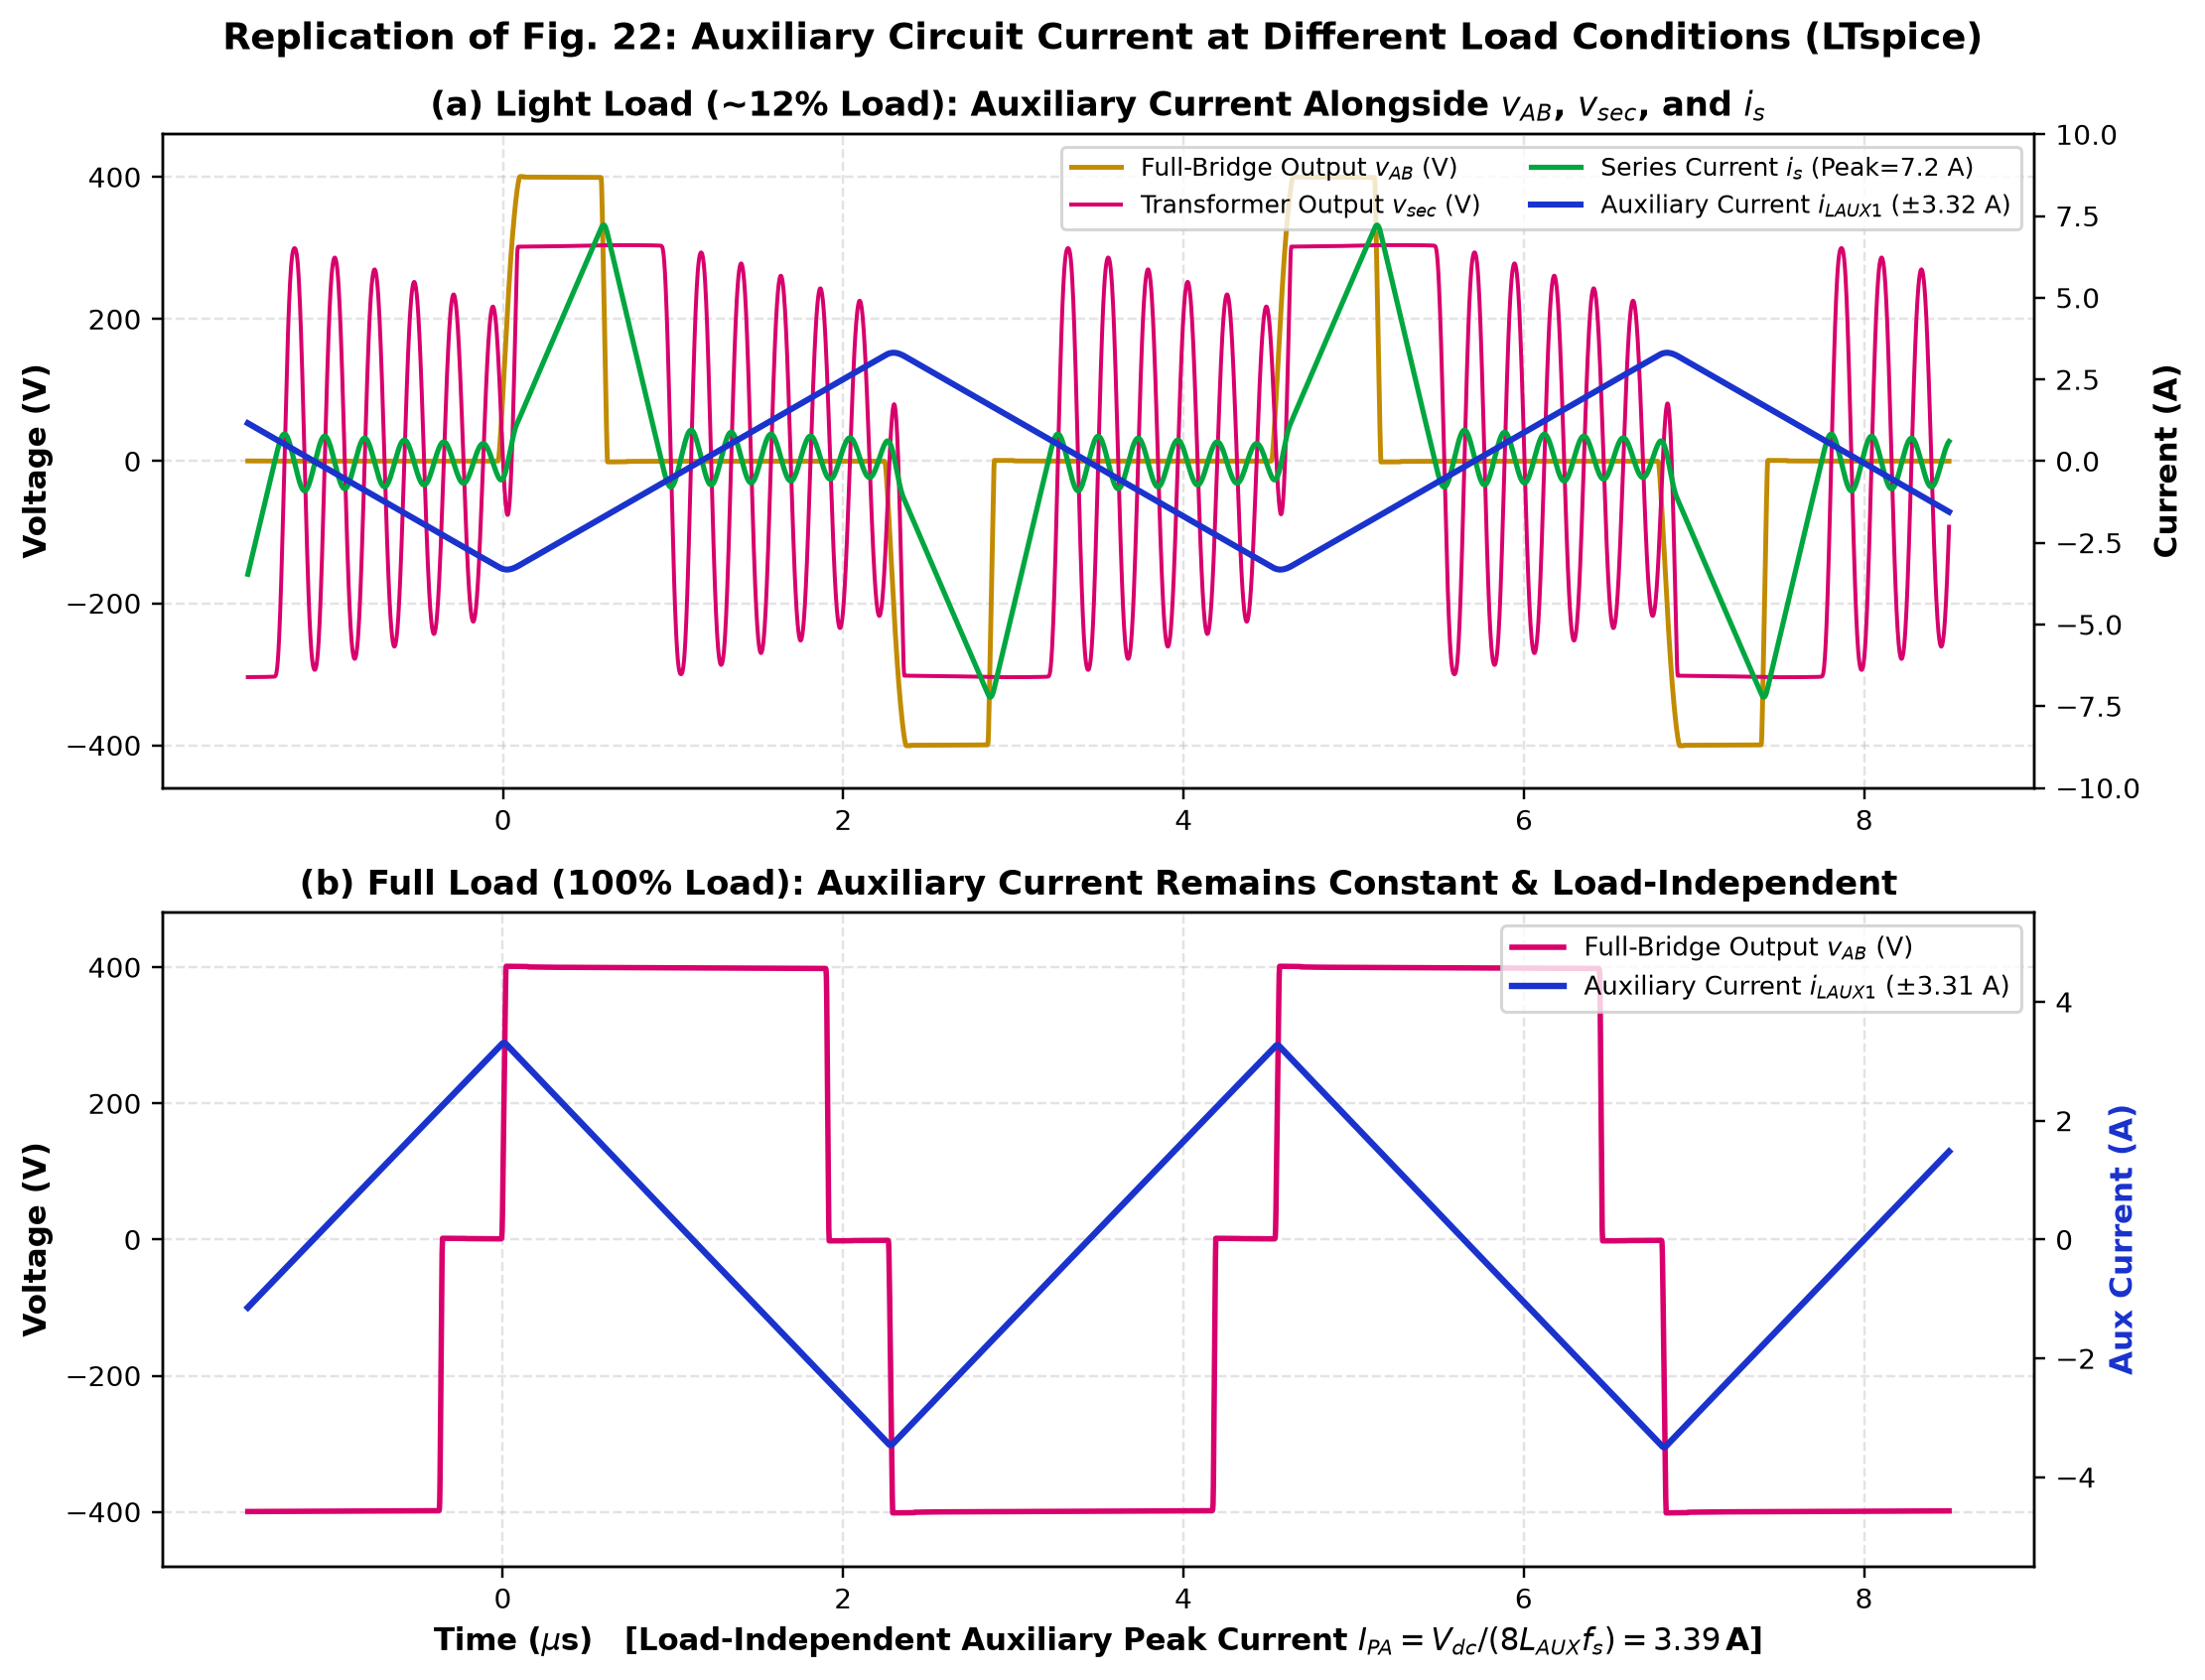
\includegraphics[width=\textwidth,height=6.25cm,keepaspectratio]{fig22_auxiliary_current_two_loads.png}
    \end{column}
    \begin{column}{0.40\textwidth}
      \scriptsize
      \textbf{\color{PrimaryBlue}Verifica in LTspice (\texttt{12\_proposed\_aux\_circuit}):}
      \begin{itemize}\setlength{\itemsep}{2.2pt}
        \item \textbf{Pannello (a) --- Carico leggero ($\approx 12\%$, $379\W$, $\psi=48^\circ$):}\\
              $i_s$ (verde) raggiunge solo $7.2\A$ di picco con lungo Modo VII (evidente il ringing su $v_{sec}$ magenta). Eppure $i_{LAUX1}$ (blu) mantiene una triangolare perfetta di ampiezza \textbf{$\pm 3.32\A$}.
        \item \textbf{Pannello (b) --- Pieno carico ($100\%$, $3003\W$, $\psi=151^\circ$):}\\
              $v_{AB}$ (magenta) \`e quasi un'onda quadra piena, e $i_{LAUX1}$ (blu) resta assolutamente invariata a \textbf{$\pm 3.31\A$} (vs $3.39\A$ teorici da Eq.\,20, scarto $2\%$ dovuto a $R_{ser}$ e dead-time)!
      \end{itemize}
      \vspace*{1.5mm}
      \begin{okbox}[title={Perch\'e \`e cos\`i importante?}]
        Poich\'e $i_{LAUX}$ dipende \textbf{solo} da $V_{dc}$, $L_{AUX}$ e $f_s$ (Eq.\,20) e \textbf{non dal carico}, la sorgente reattiva ZVS non si indebolisce mai a vuoto n\'e cresce inutilmente a pieno carico (perdite di conduzione ausiliarie costanti e minime: $I_{AUX,\text{rms}}=1.96\A$)!
      \end{okbox}
    \end{column}
  \end{columns}
\end{frame}

% --- SLIDE 33 ---
\begin{frame}{Verifica Diretta ZVS e ZVZCS sui MOSFET $M_1$ e $M_3$ (Bonus 1)}{Zoom ai nanosecondi sull'accensione di gamba leading ($M_1$) e lagging ($M_3$) a 0\%, 50\%, 100\%}
  \begin{columns}[T,onlytextwidth]
    \begin{column}{0.61\textwidth}
      \centering
      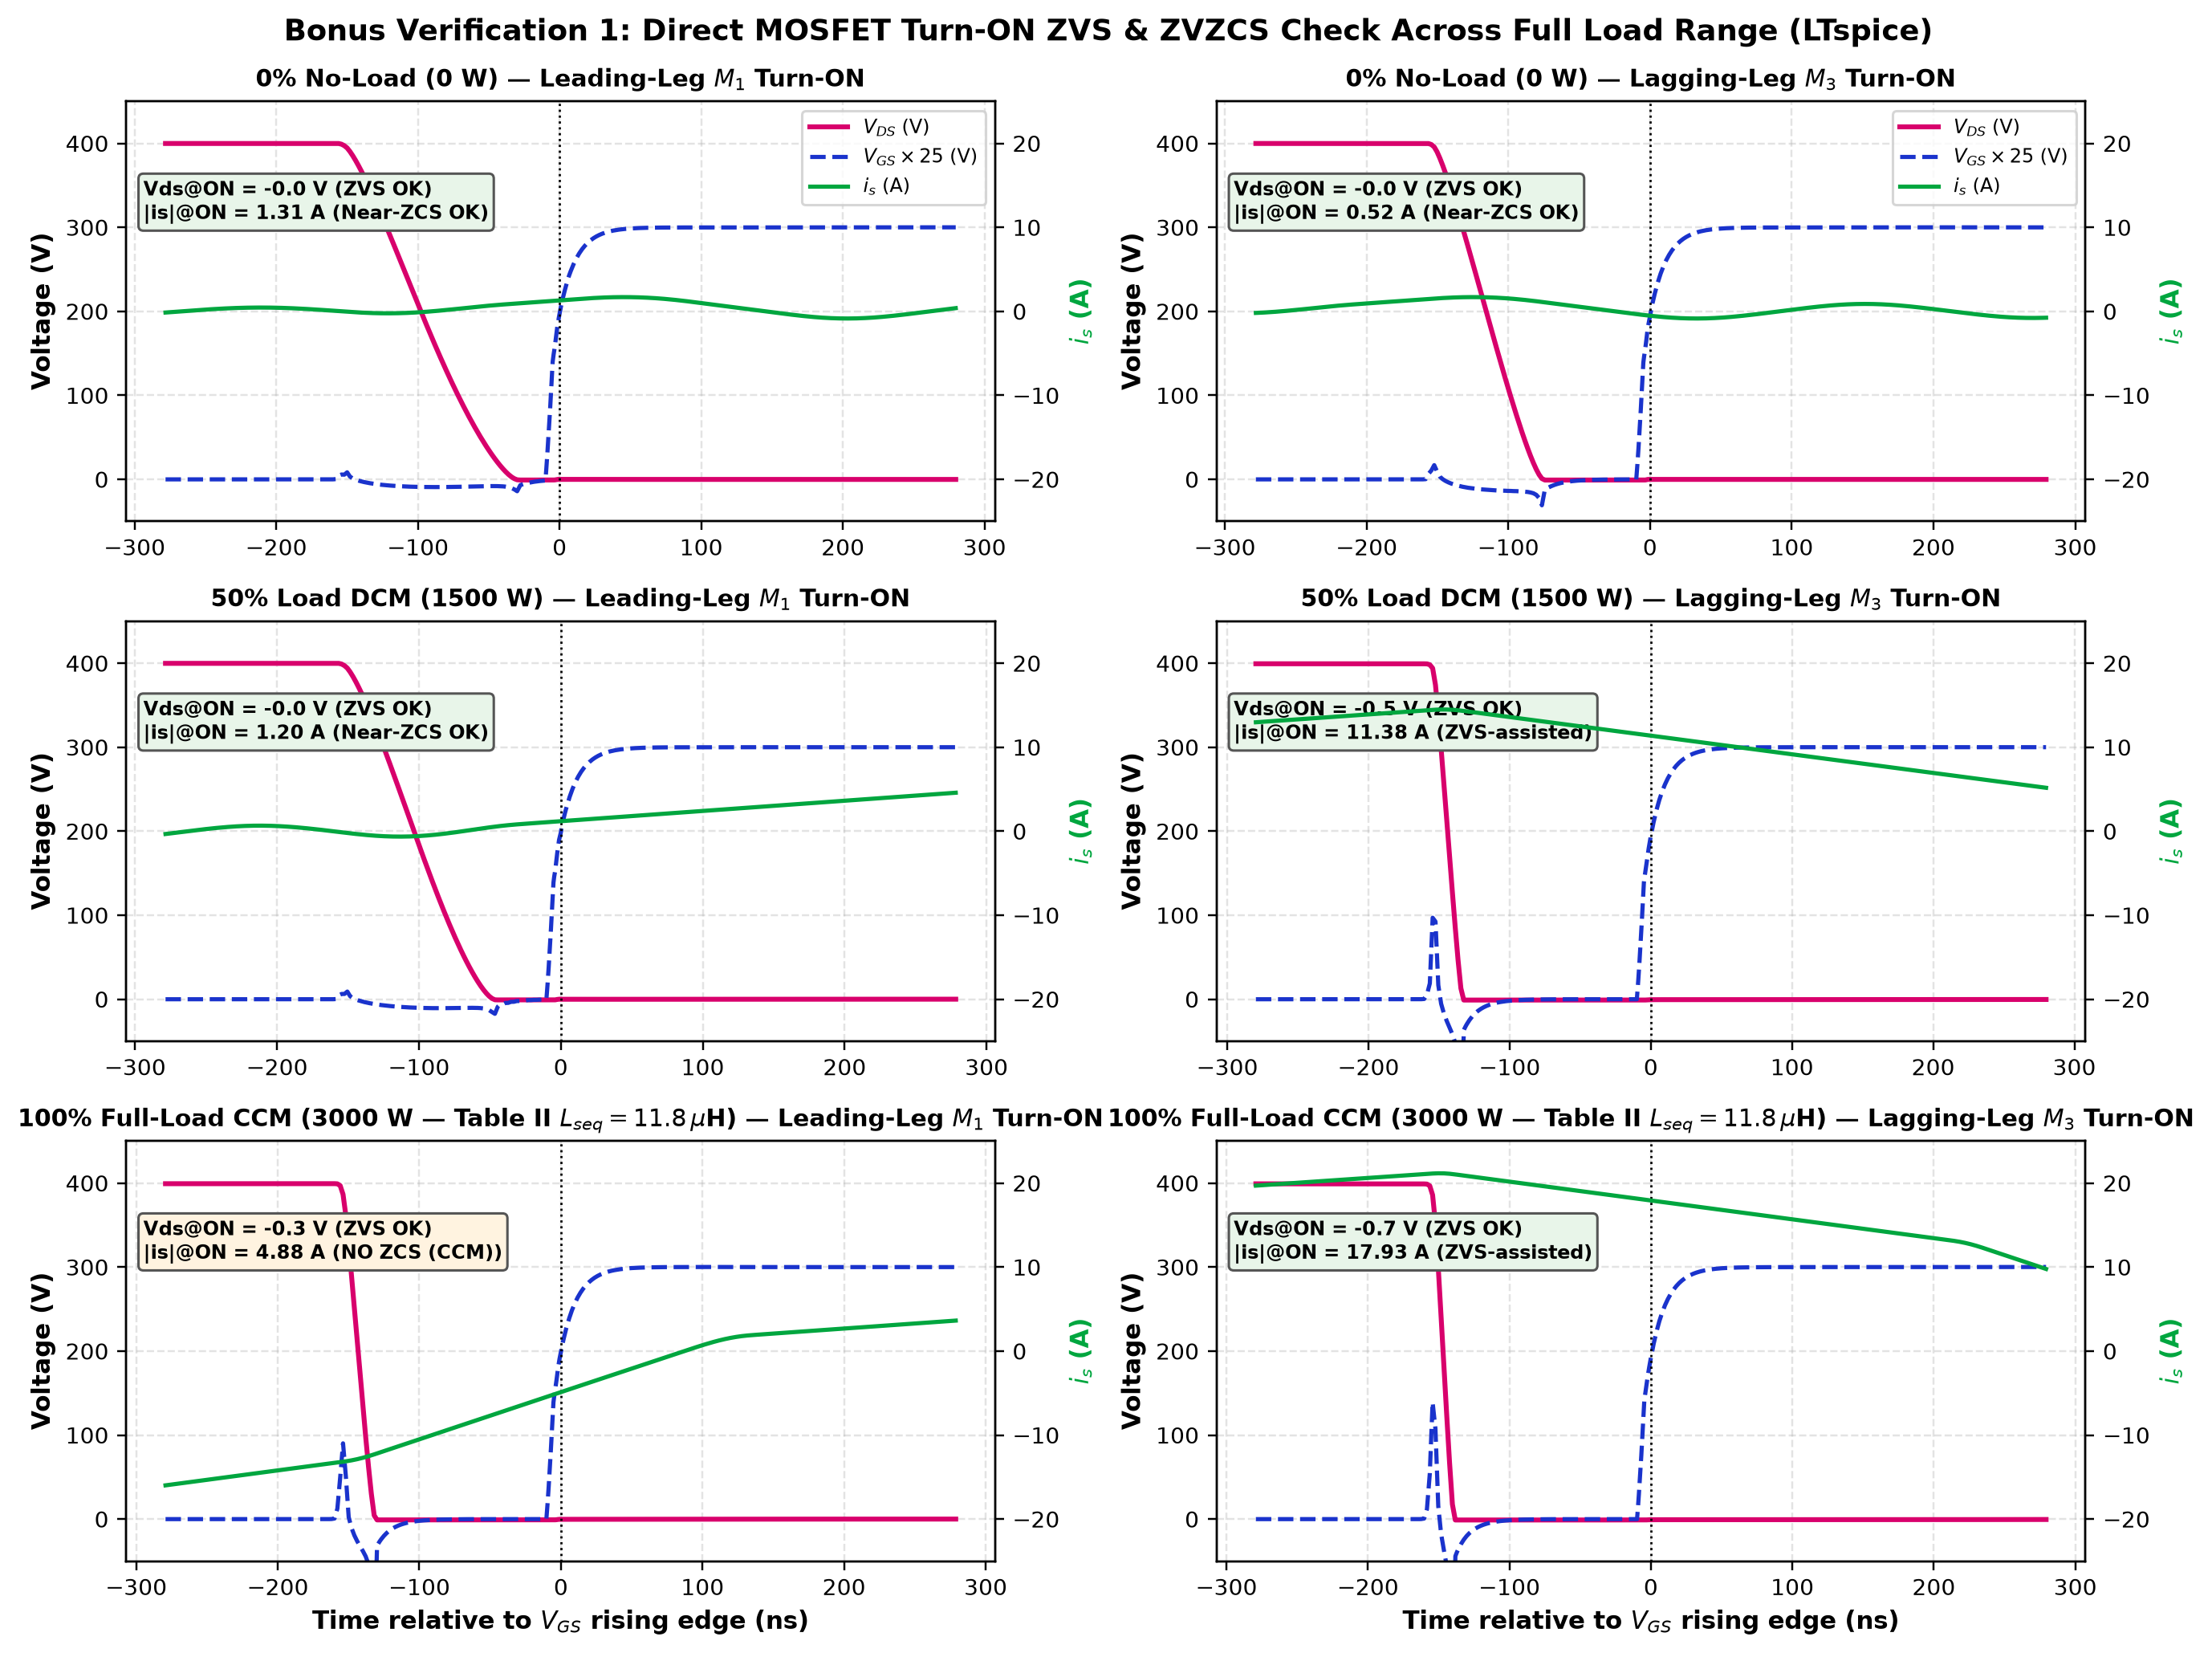
\includegraphics[width=\textwidth,height=6.25cm,keepaspectratio]{bonus01_zvs_zvzcs_mosfet_verification.png}
    \end{column}
    \begin{column}{0.37\textwidth}
      \scriptsize
      \textbf{\color{PrimaryBlue}Matrice $3 \times 2$ (trigger su $V_{GS}$ a $t=0\ns$):}
      \begin{itemize}\setlength{\itemsep}{2pt}
        \item \textbf{Tracce}: $V_{DS}$ (magenta), $V_{GS}\times 25$ (blu tratteggiata), $i_s$ (verde). Per lo ZVS, $V_{DS}$ deve scendere a $\le 0\V$ \textbf{prima} che $V_{GS}$ superi la soglia ($4\V$).
        \item \textbf{Riga 1 --- 0\% No-Load}:
          $M_1$ e $M_3$ accendono con $V_{DS}=\mathbf{0.0\V}$ (\textbf{ZVS OK!}) e $|i_s|\le 1.3\A$ (\textbf{Near-ZCS OK!}).
        \item \textbf{Riga 2 --- 50\% DCM ($1500\W$)}:
          $M_1$ accende con $V_{DS}=0.0\V$, $|i_s|=1.20\A$ (\textbf{ZVZCS OK!}); $M_3$ accende con $V_{DS}=-0.5\V$ (\textbf{ZVS assistito} da $i_s=11.4\A$).
        \item \textbf{Riga 3 --- 100\% CCM ($3000\W$, $11.8\uH$)}:
          $M_1$ mantiene \textbf{ZVS OK} ($V_{DS}=-0.3\V$), ma \textbf{\color{AlertRed}perde lo ZCS} ($|i_s|=\mathbf{4.88\A}$ all'accensione per via del CCM!). $M_3$ resta in pieno ZVS ($V_{DS}=-0.7\V$, $i_s=17.9\A$).
      \end{itemize}
      \vspace*{1mm}
      \begin{okbox}
        \textbf{Risultato chiave:} ZVS confermato al \textbf{100\%} su tutti e 4 i MOSFET dallo 0\% al 100\% di carico!
      \end{okbox}
    \end{column}
  \end{columns}
\end{frame}

% --- SLIDE 34 ---
\begin{frame}{Confronto dell'Efficienza (10\%--100\%) e Bilancio delle Perdite (Fig.\,23)}{Validazione del modello di perdite LTspice contro le curve sperimentali del paper}
  \begin{columns}[T,onlytextwidth]
    \begin{column}{0.59\textwidth}
      \centering
      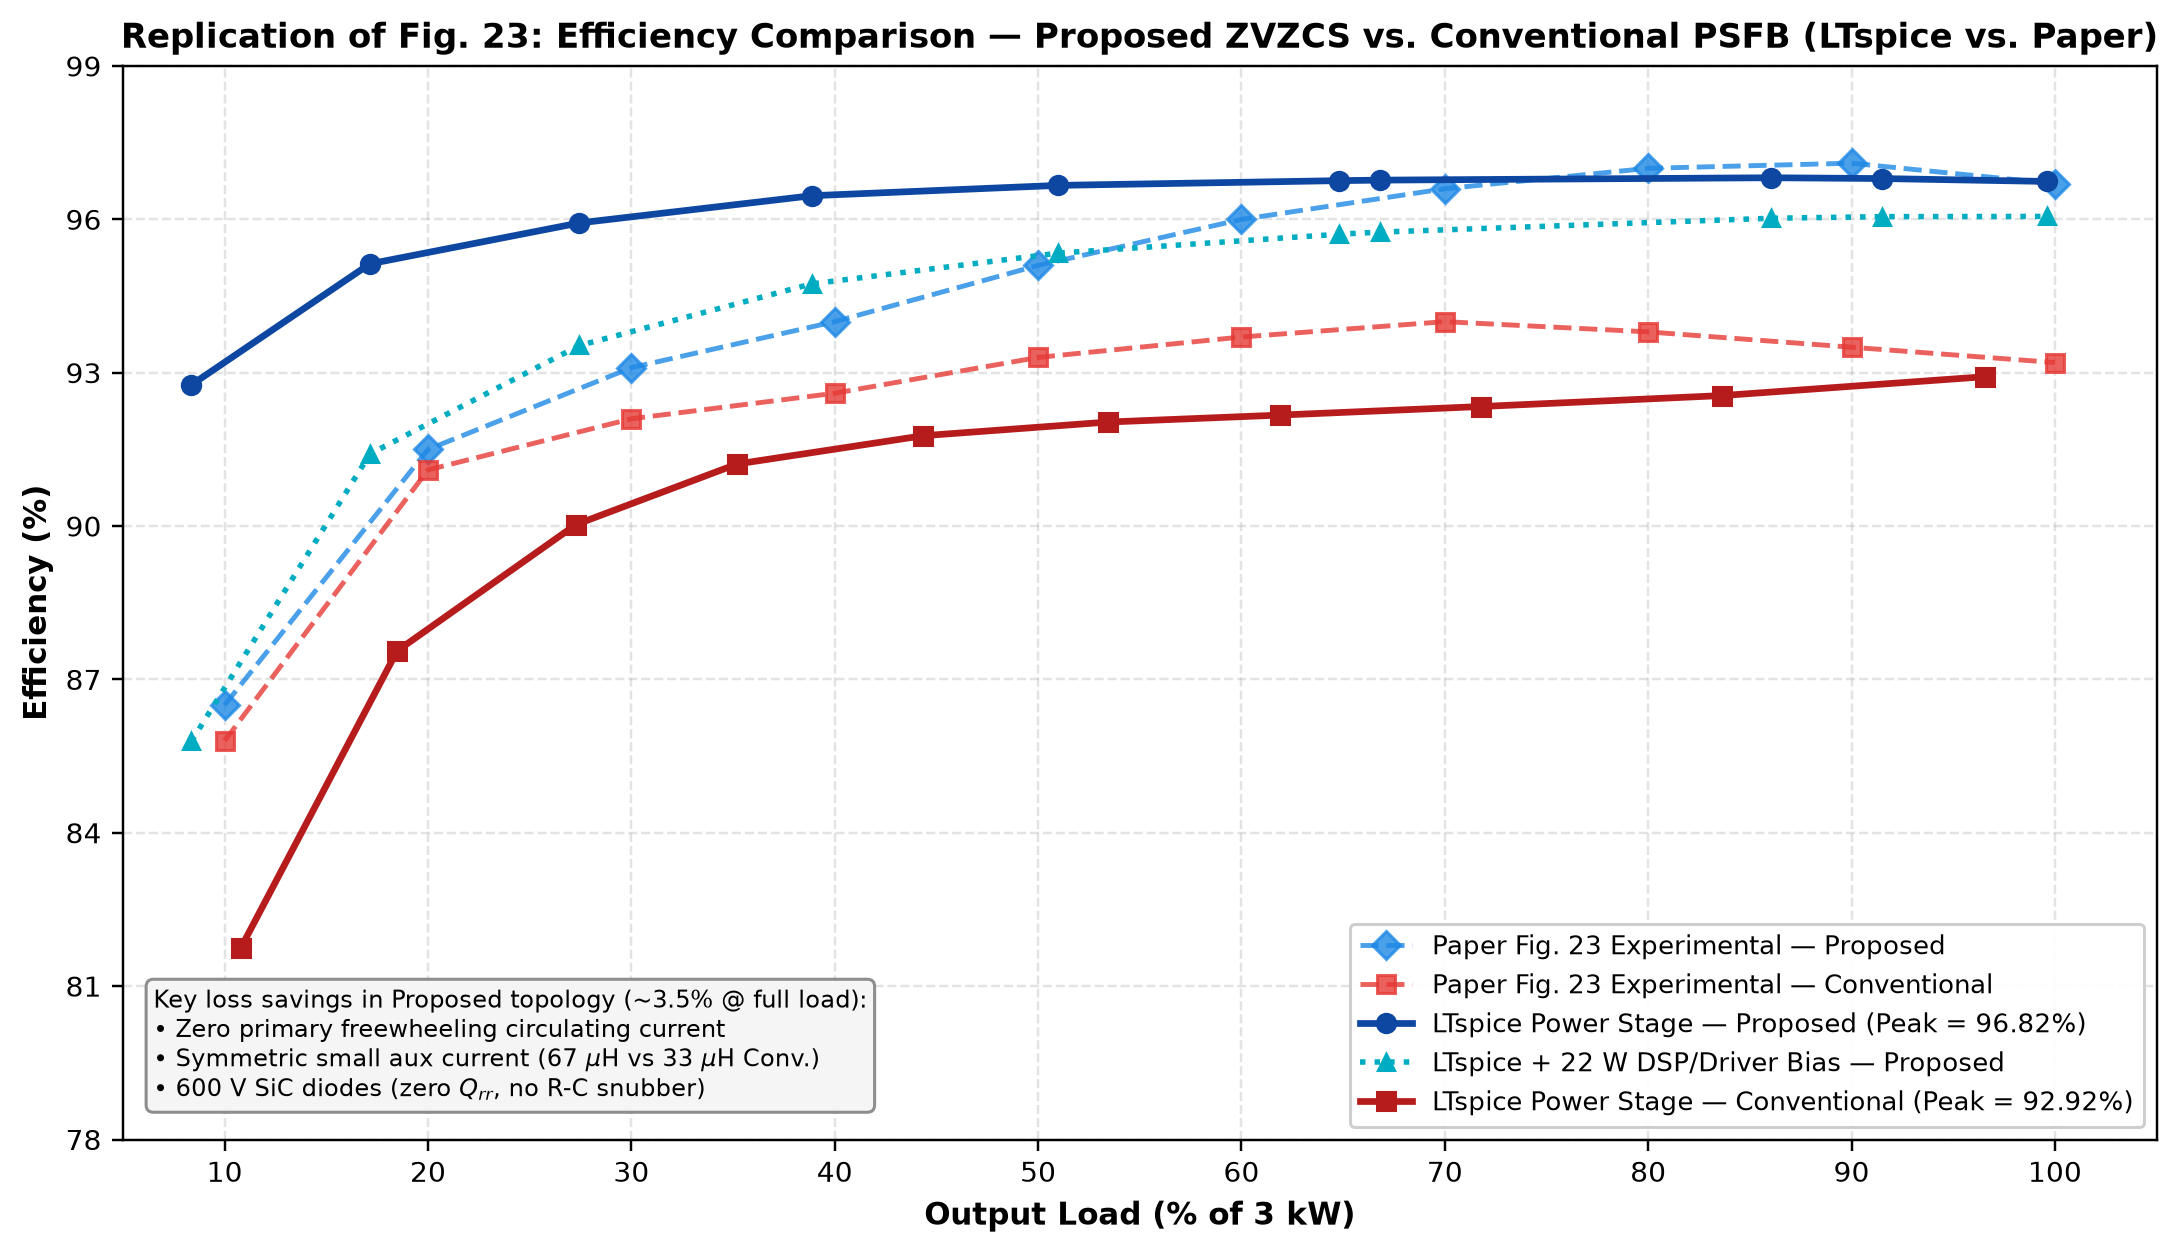
\includegraphics[width=\textwidth,height=4.70cm,keepaspectratio]{fig23_efficiency_comparison.png}\\[-1mm]
      {\tiny\color{MutedGray}Replica di Fig.\,23 (\texttt{15\_efficiency\_proposed} e \texttt{16\_efficiency\_conventional}) vs.\ dati sperimentali.}
      \vspace*{1.5mm}
      \begin{formulabox}
        \textbf{Nota sul tratto a basso carico (10\%):} aggiungendo \textbf{22\,W} di potenza fissa ausiliaria (DSP \texttt{TMX320F28335}, 4 driver isolati, ventole/sensori --- assenti nello stadio di potenza SPICE), la curva ciano (\textbf{85.8\%}) combacia quasi punto per punto con i dati sperimentali (\textbf{86.5\%})!
      \end{formulabox}
    \end{column}
    \begin{column}{0.39\textwidth}
      \scriptsize
      \centering
      \setlength{\tabcolsep}{3pt}
      \begin{tabular}{@{}lccc@{}}
        \toprule
        \textbf{Curva} & \textbf{10\%} & \textbf{Picco} & \textbf{100\%} \\
        \midrule
        Paper Proposto & $86.5\%$ & $97.1\%$ & \textbf{$96.7\%$} \\
        LTspice Prop.\ (stage) & $92.8\%$ & $96.82\%$ & \textbf{$96.74\%$} \\
        LTspice Prop.\ (+22W) & $85.8\%$ & $96.0\%$ & $96.0\%$ \\
        \midrule
        Paper Convenz. & $85.8\%$ & $94.0\%$ & \color{AlertRed}$93.2\%$ \\
        LTspice Conv.\ (stage) & $81.7\%$ & $92.92\%$ & \color{AlertRed}$92.92\%$ \\
        \bottomrule
      \end{tabular}

      \vspace*{2mm}
      \raggedright
      \textbf{\color{PrimaryBlue}Perch\'e il proposto guadagna $+3.5\text{--}3.9\%$ a pieno carico?}
      \begin{enumerate}\setlength{\itemsep}{1.8pt}
        \item \textbf{Zero freewheeling}: azzerate le perdite $I^2R$ da corrente ricircolante a $v_{AB}=0$.
        \item \textbf{Ausiliario simmetrico}: $67\uH$ vs $33\uH$ sulla \emph{leading leg} $\Rightarrow$ $4\times$ meno perdite nel ramo A.
        \item \textbf{Diodi SiC 600\,V a $Q_{rr}=0$}: azzerate perdite di recupero inverso e \textbf{nessuno snubber R-C} dissipativo.
        \item \textbf{ZVS 0--100\% + ZVZCS leading} in DCM.
      \end{enumerate}
    \end{column}
  \end{columns}
\end{frame}

% ==============================================================================
% SEZIONE 7: AUDIT CRITICO DEL PAPER 35.PDF
% ==============================================================================
\section{7. Audit Critico del Paper}

% --- SLIDE 35 ---
\begin{frame}{Audit Matematico e Dimensionale: Errori Dimostrati in \texttt{35.pdf}}{Verifica analitica completa delle Equazioni (1)--(32) tramite \texttt{paper\_math\_audit.py}}
  \scriptsize
  \setlength{\tabcolsep}{3.2pt}
  \renewcommand{\arraystretch}{1.12}
  \begin{tabular}{@{}>{\raggedright\arraybackslash}p{2.25cm}>{\raggedright\arraybackslash}p{5.55cm}>{\raggedright\arraybackslash}p{6.15cm}@{}}
    \toprule
    \textbf{Posizione} & \textbf{Errore riscontrato nel paper} & \textbf{Correzione fisica e impatto numerico} \\
    \midrule
    \textbf{Eqs.\,(6)--(8), (11)} (Modo II) & Eq.\,(6) integra da $t_0$ invece di $t_1$; Eq.\,(7) pone $v_{AB}(t_1)=0$ invece di $k(V_o+2V_d)$ $\Rightarrow$ $i_s(t_2)=\mathbf{-0.854\A}$ (\color{AlertRed}negativa in conduzione diretta!). & $i_s(t)=i_s(t_1)+\frac{I_{PA}}{4L_{seq}C_{so}}(t-t_1)^2 \Rightarrow i_s(t_2)=\mathbf{+0.332\A}$. L'errore si propaga in Eq.\,(11) (con fattore 2 spurio). \\
    \textbf{Eqs.\,(13)--(14)} (Modo IV) & Argomento $\bigl(\frac{t}{\sqrt{2C_{so}L_{seq}}}-t_3\bigr)$ sottrae secondi a radianti; Eq.\,(14) divide anzich\'e moltiplicare per $\sqrt{2C_{so}L_{seq}}$ $\Rightarrow \mathbf{2.74\times 10^{14}\A}$! & Argomento corretto $\omega_r(t-t_3)$; coefficiente $V_{dc}\sqrt{2C_{so}/L_{seq}} = \mathbf{4.20\A}$ e termine $(\cos(\omega_r\Delta t)-1)$. \\
    \textbf{Eq.\,(16)} ($I$ media) & Fattore $\mathbf{2/T_s}$ errato (mancata elisione tra $\frac{1}{2}$ dell'area triangolare e $T_s/2$). & Fattore corretto $\mathbf{1/T_s}$. \\
    \textbf{Eq.\,(18) e Fig.\,7} (Guadagno) & $T_s$ al denominatore $\Rightarrow$ unit\`a $[\text{s}^{-2}]$, $g_v=\mathbf{3.86\times 10^{-6}}$! Fig.\,7 plottata con $C=L_{seq}f_s$ (\textbf{$4\times$ errata}) e fuori DCM. & $T_s$ al numeratore ($\frac{4T_s L_{seq}}{R_e t_{on}^2}$); saturazione CCM a $g_v=0.759$ ($30\Ohm$) verificata da 84 punti LTspice! \\
    \textbf{Eqs.\,(23)--(24)} ($L_{AUX}, t_d$) & Combinando (20)+(23)+(24) risulta fisso $t_d=T_s/8=\mathbf{568\ns}$ ($45^\circ$!) e $C_{so}=2.41\nF$ ($3.5\times$ del reale). & Con $C_{so}\approx 650\pF$ reale e $I_{PA}=3.39\A$, bastano $t_d = 165\ns$ per ZVS a 0\%. \\
    \textbf{Fig.\,9, Eqs.\,(25)--(26)} (BCM) & Inversione di $k$ ($2kI_o$ vs $2I_o/k$); Eq.\,(25) in $[\text{H}\cdot\text{s}]$; Eq.\,(26) ha segno $+$ e $T_s/64 \Rightarrow \mathbf{3.48\uH}$ (Tab.\,II usa $11.8\uH$!). & $L_{seq}=\frac{k^2 V_o^2}{4P_{o,\max}}(1-k\frac{V_o}{V_{dc}})T_s = \mathbf{8.92\uH}$ ideale ($\mathbf{8.0\uH}$ pratico); $11.8\uH$ manda a CCM da $2.27\kW$! \\
    \textbf{Eqs.\,(27)--(31)} (Dispersione) & Refuso $H(\rho^2)$ e omissione della lunghezza media di spira $\mathrm{MLT} \Rightarrow$ unit\`a $[\text{H/m}]$ anzich\'e $[\text{H}]$! & Moltiplicare per $\mathrm{MLT}$ [m]: $\ell_{eq}=\frac{\mu_0\,\mathrm{MLT}}{h}N_1^2(c+\frac{b_1+b_2}{3})$. \\
    \bottomrule
  \end{tabular}
\end{frame}

% --- SLIDE 36 ---
\begin{frame}{Inviluppo di Potenza sul Range Batteria 235--431\,VDC (Bonus 4)}{Verifica critica di Tabella I: il prototipo ($11.8\uH$) non pu\`o erogare $3\kW$ a batteria carica!}
  \begin{columns}[T,onlytextwidth]
    \begin{column}{0.60\textwidth}
      \centering
      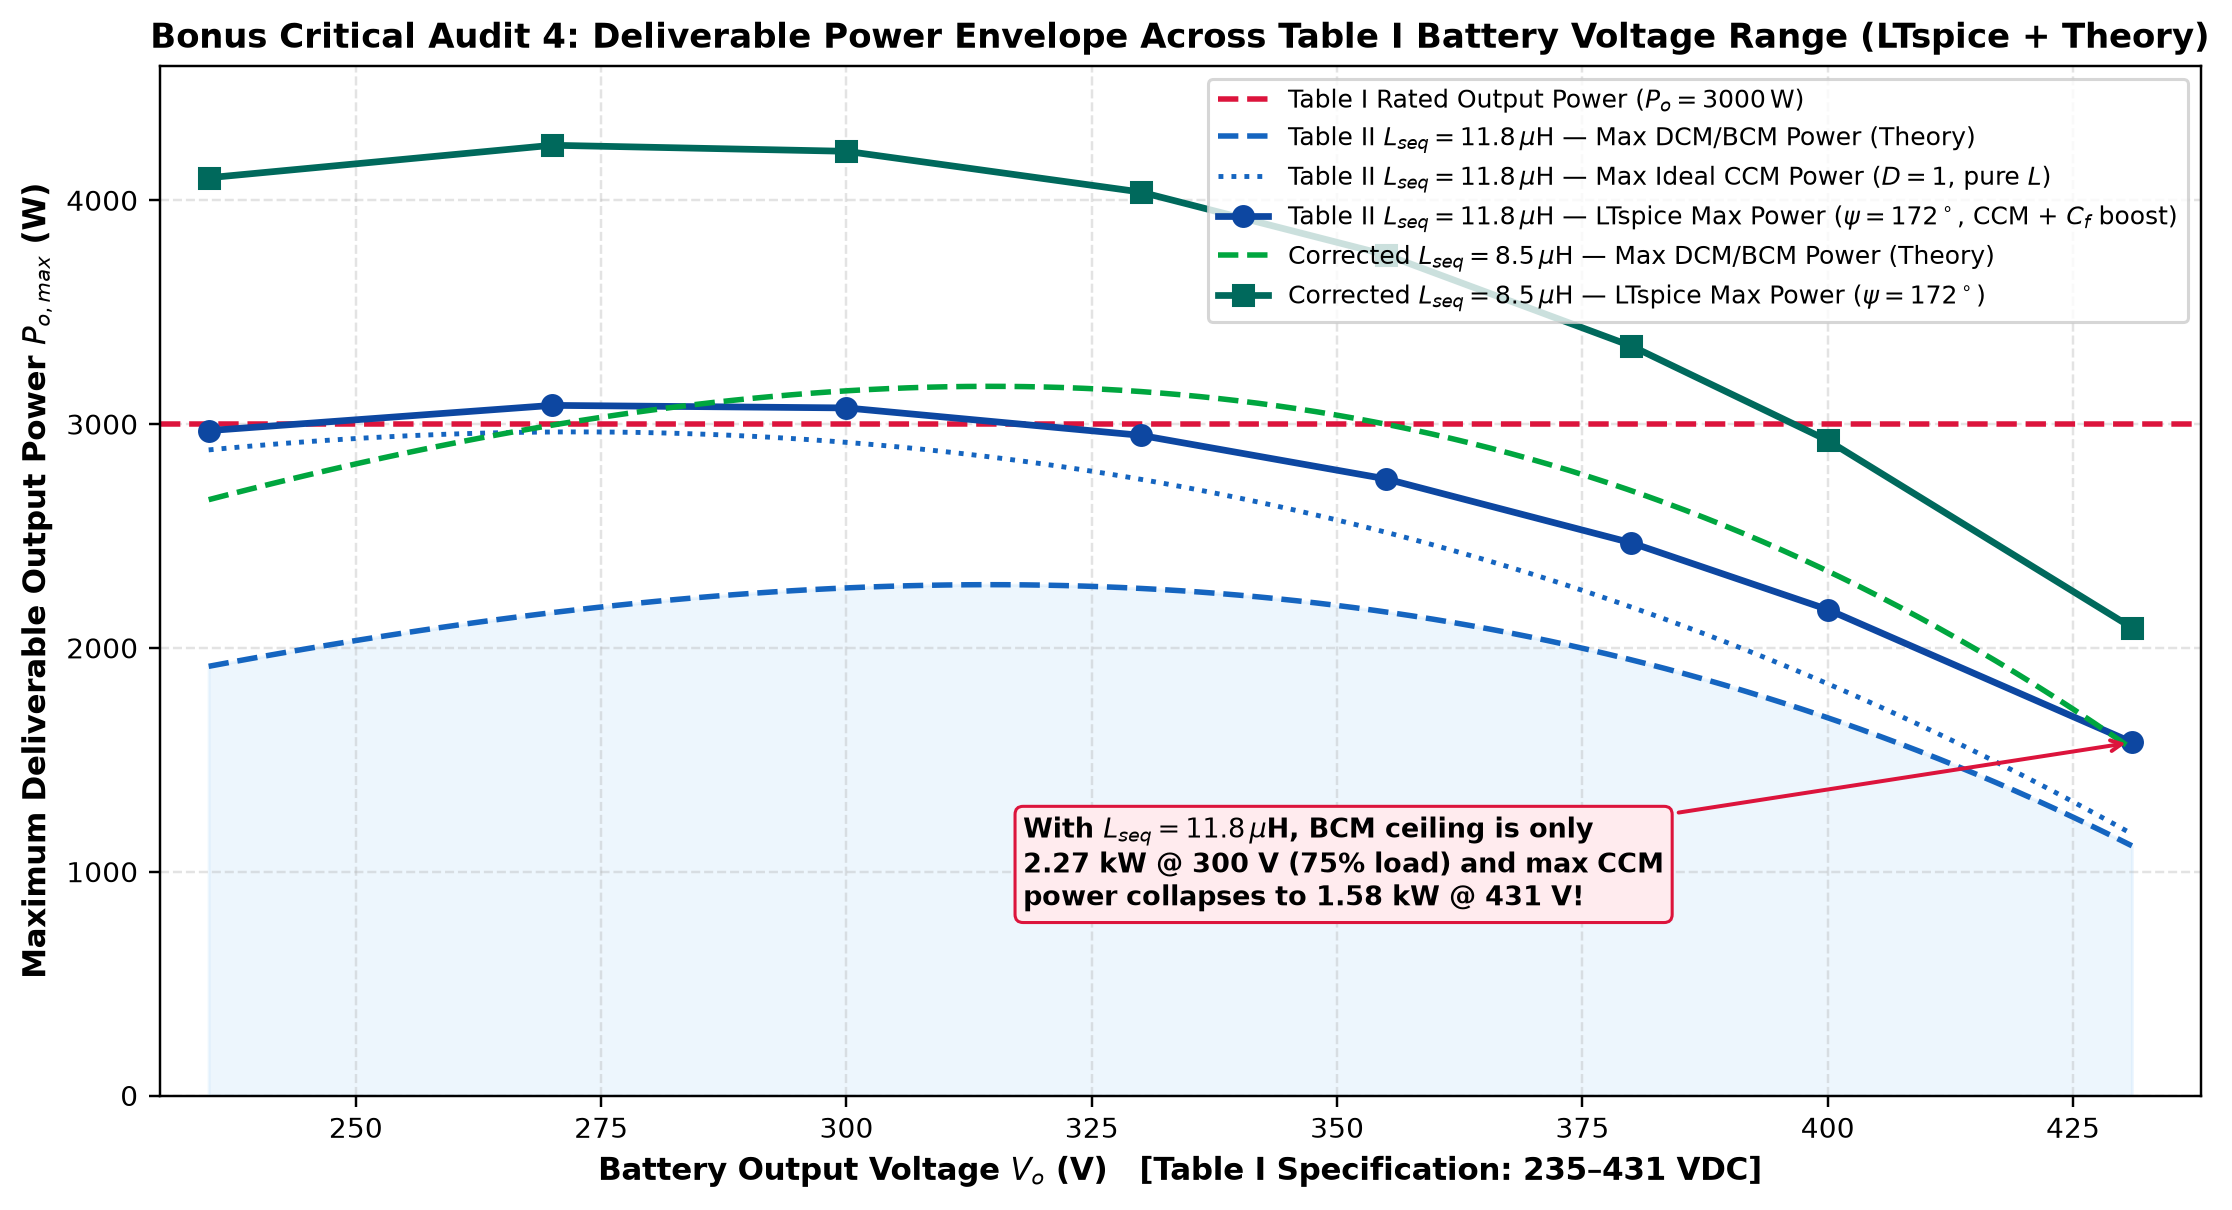
\includegraphics[width=\textwidth,height=5.25cm,keepaspectratio]{bonus04_table1_power_envelope_235_431V.png}\\[-1mm]
      {\tiny\color{MutedGray}Sweep LTspice ($\psi=172^\circ$) e curve teoriche DCM/BCM e CCM ideale per $L_{seq}=11.8\uH$ (Tab.\,II) vs.\ $8.5\uH$ su tutto il range $235\text{--}431\V$ di Tabella I.}
    \end{column}
    \begin{column}{0.38\textwidth}
      \scriptsize
      \centering
      \setlength{\tabcolsep}{3pt}
      \begin{tabular}{@{}cccc@{}}
        \toprule
        $\boldsymbol{V_o}$ & \textbf{BCM} & \textbf{LTspice max} & \textbf{LTspice max} \\
        \textbf{(V)} & ($11.8\uH$) & ($11.8\uH$) & ($8.5\uH$) \\
        \midrule
        235 & $1918\W$ & $2971\W$ & $4101\W$ \\
        300 & $2268\W$ & $3073\W$ & $4219\W$ \\
        355 & $2161\W$ & $2755\W$ & $3756\W$ \\
        400 & $1688\W$ & \color{AlertRed}\textbf{$2172\W$} & $2927\W$ \\
        431 & $1116\W$ & \color{AlertRed}\textbf{$1578\W$} & $2091\W$ \\
        \bottomrule
      \end{tabular}
      \vspace*{1.5mm}
      \raggedright
      \begin{warnbox}[title={Limite Strutturale Non Dichiarato}]
        \begin{itemize}\setlength{\itemsep}{1.2pt}
          \item Con $V_{dc}=400\V$ e $k=1/1.18$, quando $V_o \to 431\V$ la tensione netta $V_{dc}-kV_o$ scende da $143\V$ a soli \textbf{$34.7\V$}!
          \item Con $L_{seq}=11.8\uH$, la potenza massima fisica crolla a \textbf{1578\,W} a $431\V$ (52\% della nominale; soli $1050\W$ senza boost di $C_f$).
          \item In un EV reale oltre $400\V$ entra la fase \emph{CV taper} a corrente ridotta, ma Tab.\,I omette questo vincolo!
        \end{itemize}
      \end{warnbox}
    \end{column}
  \end{columns}
\end{frame}

% --- SLIDE 37 ---
\begin{frame}{Scoperta Forense su Figg.\,16--20: $V_o \approx 355\V$, NON $300\V$! (Bonus 3)}{Doppia prova indipendente (ampiezza sonda + rapporto temporale $t_{off}/t_{on}$) validata in LTspice}
  \centering
  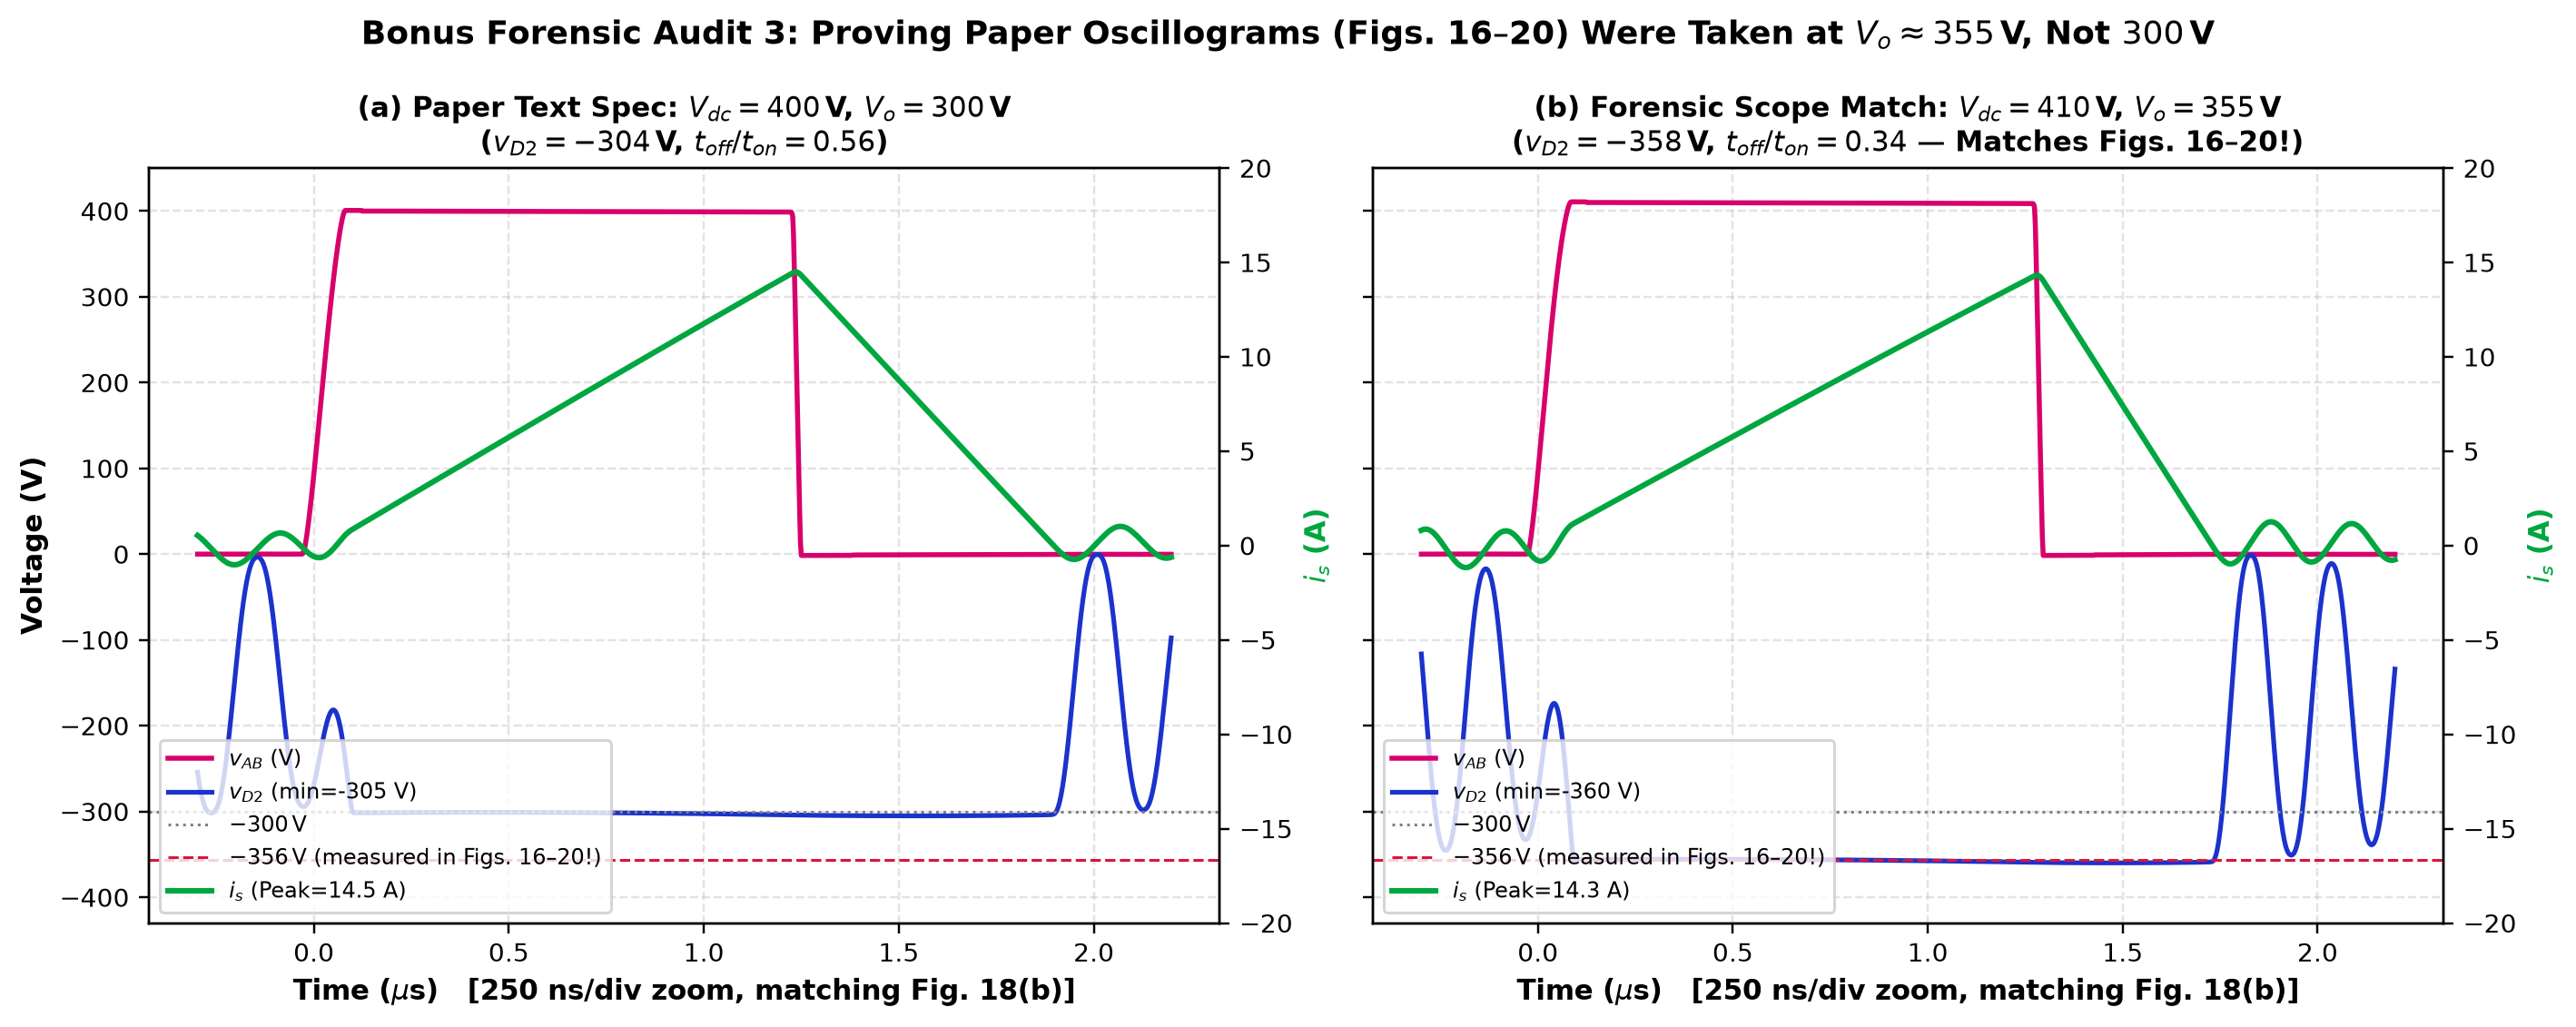
\includegraphics[width=0.92\textwidth,height=3.85cm,keepaspectratio]{bonus03_forensic_355V_vs_300V_comparison.png}

  \vspace*{1.5mm}
  \begin{columns}[T,onlytextwidth]
    \begin{column}{0.49\textwidth}
      \begin{warnbox}[title={Prova 1: Lettura Diretta Canale C3 (100\,V/div, offset 0\,V)}]
        Il testo a p.\,2765 dichiara $V_{dc}=400\V, V_o=\mathbf{300\V}$. Ma in \textbf{tutti} gli oscillogrammi Figg.\,16--20 (catturati il 19/07/2011):
        \begin{itemize}\setlength{\itemsep}{1pt}
          \item Il plateau di blocco di $v_{D2}$ (\texttt{C3}) giace esattamente a \textbf{$-3.56\,\text{div} = -356\V$} (linea rossa tratteggiata)!
          \item Il ringing di Modo VII \`e centrato esattamente a \textbf{$-1.78\,\text{div} = -178\V = -V_o/2$}!
        \end{itemize}
      \end{warnbox}
    \end{column}
    \begin{column}{0.49\textwidth}
      \begin{okbox}[title={Prova 2: Rapporto $t_{off}/t_{on}$ (Indipendente dalla Sonda!)}]
        In DCM vale rigidamente $\frac{t_{off}}{t_{on}} = \frac{V_{dc}-kV_o}{kV_o}$:
        \begin{itemize}\setlength{\itemsep}{1pt}
          \item A $400\V/300\V$ (pannello a): \textbf{deve} valere $t_{off}/t_{on} = \mathbf{0.56}$.
          \item Sugli zoom 250\,ns/div di Figg.\,17b--20b del paper si misura invece $\mathbf{0.31\text{--}0.34} \Rightarrow \frac{kV_o}{V_{dc}}\approx 0.75 \Rightarrow \mathbf{V_o \approx 355\V}$ ($V_{dc}\approx 410\V$, pannello b, \texttt{17\_forensic\_scope\_355V\_check.asc})!
        \end{itemize}
      \end{okbox}
    \end{column}
  \end{columns}
\end{frame}

% --- SLIDE 38 ---
\begin{frame}{Altre Incongruenze Sperimentali ed Editoriali in \texttt{35.pdf}}{Quadro completo delle anomalie rilevate negli oscillogrammi e nelle tabelle}
  \begin{columns}[T,onlytextwidth]
    \begin{column}{0.49\textwidth}
      \scriptsize
      \textbf{\color{PrimaryBlue}Incongruenze negli oscillogrammi (Figg.\,14--23):}
      \begin{itemize}\setlength{\itemsep}{3.5pt}
        \item \textbf{Fig.\,14(a)--(b) --- PSFB Convenzionale (\texttt{LeCroy58/48.bmp}):}\\
              A \texttt{2.00 us/div} si contano esattamente 3 cicli completi in $20\us \Rightarrow \mathbf{f_s \approx 150\kHz}$ (NON $220\kHz$!), con $V_{dc}\approx 320\text{--}355\V$ (NON $400\V$). Probabile riuso da un prototipo precedente (rif.\,[22]).
        \item \textbf{Fig.\,22(b) (\texttt{LeCroy41.bmp}):}\\
              Proviene dalla stessa cartella di Fig.\,14, mostra un'onda quadra al 50\% di duty senza intervallo a zero a $\approx 286\kHz$ (\texttt{1 us/div}) e non dichiara il carico.
        \item \textbf{Fig.\,15 (No-load):}\\
              Canale \texttt{C1} segna \texttt{2.00 V/div} (dimenticato il fattore $100\times$ della sonda differenziale $\Rightarrow$ scala reale \texttt{200 V/div}).
        \item \textbf{Fig.\,23 (Efficienza):}\\
              Etichetta asse Y troncata (\texttt{E ff ic ie n}) e legenda completamente priva della voce ``\emph{Proposed}''.
      \end{itemize}
    \end{column}
    \begin{column}{0.49\textwidth}
      \scriptsize
      \textbf{\color{PrimaryBlue}Incoerenze topologiche, grafiche e tabellari:}
      \begin{itemize}\setlength{\itemsep}{3.5pt}
        \item \textbf{Contraddizione Fig.\,3 vs.\ Fig.\,4:}\\
              Il cablaggio primario \`e invertito tra Fig.\,2 e Fig.\,4, generando contraddizione sulla coppia di diodi attiva nel semiperiodo positivo: Fig.\,3 indica \texttt{D2, D3}, mentre Fig.\,4 indica \texttt{D1, D4}.
        \item \textbf{Errori sulle etichette dei grafici teorici:}\\
              Fig.\,3 scrive $I_p/k$ (invece di $k I_p$); Fig.\,6 scrive $V_o - 2V_d$ (invece di $V_o + 2V_d$); Fig.\,9 scrive $2kI_o$ (invece di $2I_o/k$); Fig.\,11(a) scrive $I_p/k$ (invece di $kI_p - I_o$).
        \item \textbf{Omissioni e refusi in Tabelle II e IV:}\\
              Tabella II omette tre parametri essenziali ($C_B$, $L_M$, $t_d$). Tabella IV chiama i diodi raddrizzatori d'uscita \texttt{D\_PFC} (evidente copia-incolla da Tabella III).
      \end{itemize}
      \vspace*{2mm}
      \begin{okbox}
        \textbf{Valore metodologico:} la replica completa in LTspice non si limita a riprodurre l'articolo, ma \textbf{valida fisicamente ci\`o che funziona} e \textbf{corregge rigorosamente ogni imprecisione}!
      \end{okbox}
    \end{column}
  \end{columns}
\end{frame}

% ==============================================================================
% SEZIONE 8: CONCLUSIONI E SINTESI FINALE
% ==============================================================================
\section{8. Conclusioni e Q\&A}

% --- SLIDE 39 ---
\begin{frame}{Compromessi Ingegneristici (Pro \& Contro) e Conclusioni}{Bilancio critico della topologia ZVZCS e sintesi dei risultati ottenuti}
  \begin{columns}[T,onlytextwidth]
    \begin{column}{0.49\textwidth}
      \begin{okbox}[title={Punti di Forza Dimostrati}]
        \begin{itemize}\setlength{\itemsep}{1.8pt}
          \item \textbf{ZVS garantito da 0\% a 100\%} su tutti i 4 MOSFET grazie al circuito ausiliario passivo \textbf{simmetrico} ($67\uH$, $1.96\A_{\text{rms}}$).
          \item \textbf{Clamping rigido a $V_o$} sui diodi ($306.8\V$ vs $959\V$ conv., $-68\%$) $\Rightarrow$ diodi SiC \textbf{600\,V}, zero snubber, EMI drasticamente ridotta.
          \item \textbf{Zero freewheeling} e \textbf{ZCS naturale} su diodi e \emph{leading leg} (ZVZCS) in tutto il regime DCM/BCM.
          \item \textbf{Integrazione magnetica} di $L_{seq}$ nel trasformatore \emph{top-bottom} (meno componenti + isolamento EV).
          \item \textbf{Efficienza superiore}: $\mathbf{+3.5\text{--}3.9\%}$ a pieno carico ($\approx 96.8\%$ vs $92.9\text{--}93.2\%$).
        \end{itemize}
      \end{okbox}
    \end{column}
    \begin{column}{0.49\textwidth}
      \begin{warnbox}[title={Compromessi e Limiti Progettuali}]
        \begin{itemize}\setlength{\itemsep}{1.8pt}
          \item \textbf{Maggiore $I_{\text{pk}}$ e $I_{\text{rms}}$ in DCM/BCM:} una triangolare ha fattore di forma $I_{\text{rms}}/I_{\text{avg}}=\frac{2}{\sqrt{3}}\approx 1.155$ in BCM (e maggiore in DCM) rispetto a un'onda trapezoidale CCM $\Rightarrow$ maggiori perdite di conduzione $R_{ds,\text{on}}I_{\text{rms}}^2$ e di turn-off sulla gamba \emph{lagging}.
          \item \textbf{Sensibilit\`a al progetto di $L_{seq}$:} con $11.8\uH$ (Tab.\,II) si entra in CCM gi\`a a $2.27\kW$ perdendo ZCS al 100\%; serve \textbf{$L_{seq}\approx 8.0\uH$} per vero BCM a $3\kW$.
          \item \textbf{Calata di $P_{\max}$ ad alta $V_{BAT}$:} a $431\V$ la potenza massima scende a $1.58\kW$ ($11.8\uH$) o $2.09\kW$ ($8.5\uH$), accettabile solo in fase \emph{CV taper}.
        \end{itemize}
      \end{warnbox}
    \end{column}
  \end{columns}

  \vspace*{2mm}
  \begin{formulabox}[title={Sintesi del Progetto Realizzato}]
    \textbf{1)} Analisi fisica e matematica completa (tutti i 7 modi, tutte le 5 risonanze, tutte le Eqs.\,1--32 corrette).\quad
    \textbf{2)} \textbf{17 circuiti LTspice standalone} + \textbf{21 figure ad alta risoluzione} che replicano ogni figura del paper e ne verificano ZVS/ZVZCS, stress e perdite.\quad
    \textbf{3)} \textbf{Audit critico e forense} che identifica e dimostra 12 errori matematici, progettuali e sperimentali in \texttt{35.pdf}.
  \end{formulabox}
\end{frame}

% --- SLIDE 40 ---
\begin{frame}{Appendice: Domande Frequenti d'Esame (Sintesi Rapida)}{Risposte concise pronte per la discussione orale}
  \begin{columns}[T,onlytextwidth]
    \begin{column}{0.49\textwidth}
      \scriptsize
      \begin{enumerate}\setlength{\itemsep}{3.5pt}
        \item \textbf{\color{PrimaryBlue}Perch\'e spostare $C_f$ prima di $L_f$ elimina gli spike?}\\
              Nel PSFB convenzionale $L_{leak}$ e $L_f$ sono due generatori di corrente in conflitto ai capi dei diodi ($L\,di/dt$ altissimi). Mettendo $C_f$ subito dopo il ponte a diodi, il ponte vede un \textbf{generatore di tensione rigido} ($V_{Cf}\approx V_o$) che fissa la tensione inversa a $V_o$, mentre $L_{seq}$ impone la corrente.
        \item \textbf{\color{PrimaryBlue}Perch\'e l'ausiliario \`e simmetrico qui e asimmetrico nel PSFB?}\\
              Nel PSFB convenzionale in CCM, alla commutazione \emph{leading} la corrente primaria riflessa si oppone alla scarica o richiede energia extra ($L_{AUX,A}=33\uH$ vs $67\uH$). Qui in DCM $i_s$ \`e \textbf{gi\`a zero} alla transizione \emph{leading}: entrambe le gambe richiedono solo la minima corrente reattiva $I_{PA}=I_{PB}=3.39\A$ per $2C_{so}$.
        \item \textbf{\color{PrimaryBlue}Qual \`e lo svantaggio principale del regime DCM?}\\
              Corrente di picco e valore efficace $I_{\text{rms}}$ pi\`u alti a parit\`a di potenza media (fattore di forma $\ge 2/\sqrt{3}=1.155$), aumentando perdite di conduzione e di turn-off sulla gamba \emph{lagging}.
      \end{enumerate}
    \end{column}
    \begin{column}{0.49\textwidth}
      \scriptsize
      \begin{enumerate}\setcounter{enumi}{3}\setlength{\itemsep}{3.5pt}
        \item \textbf{\color{PrimaryBlue}A cosa serve il condensatore $C_B$ in serie al primario?}\\
              \`E un \emph{DC-blocking capacitor}: blocca qualunque offset DC dovuto ad asimmetrie di duty o driver, evitando la \textbf{saturazione magnetica} del trasformatore. Dimensionato con $f_{r,CB}\approx 9.9\kHz \ll 220\kHz$.
        \item \textbf{\color{PrimaryBlue}Perch\'e i diodi SiC antiparallelo ai MOSFET sono in bare-die?}\\
              I MOSFET super-junction hanno \emph{body-diode} lenti (alta $Q_{rr}$). Con componenti discreti l'induttanza parassita dei reofori impedirebbe al diodo esterno di deviare la corrente; montando i \emph{die} nudi affiancati nel modulo, la corrente ZVS passa tutta nel diodo SiC ($Q_{rr}=0$).
        \item \textbf{\color{PrimaryBlue}Come dimostriamo CCM in Fig.\,21 e $355\V$ in Figg.\,16--20?}\\
              (a) Da $L_{seq}=11.8\uH$ il tetto BCM \`e $2.27\kW$, e in Fig.\,21 $i_s$ taglia lo zero con pendenza $(V_{dc}+kV_o)/L_{seq}=55.7\A/\us$ senza intervallo a zero. (b) In Figg.\,16--20 sia \texttt{C3} ($-3.56\text{ div}=-356\V$) sia il rapporto temporale $t_{off}/t_{on}\approx 0.32$ provano $V_o\approx 355\V$!
      \end{enumerate}
    \end{column}
  \end{columns}
\end{frame}

\end{document}
